%% abtex2-modelo-trabalho-academico.tex, v-1.9.7 laurocesar
%% Copyright 2012-2018 by abnTeX2 group at http://www.abntex.net.br/ 
%%
%% This work may be distributed and/or modified under the
%% conditions of the LaTeX Project Public License, either version 1.3
%% of this license or (at your option) any later version.
%% The latest version of this license is in
%%   http://www.latex-project.org/lppl.txt
%% and version 1.3 or later is part of all distributions of LaTeX
%% version 2005/12/01 or later.
%%
%% This work has the LPPL maintenance status `maintained'.
%% 
%% The Current Maintainer of this work is the abnTeX2 team, led
%% by Lauro César Araujo. Further information are available on 
%% http://www.abntex.net.br/
%%
%% This work consists of the files abntex2-modelo-trabalho-academico.tex,
%% abntex2-modelo-include-comandos and abntex2-modelo-references.bib
%%

% ------------------------------------------------------------------------
% ------------------------------------------------------------------------
% abnTeX2: Modelo de Trabalho Academico (tese de doutorado, dissertacao de
% mestrado e trabalhos monograficos em geral) em conformidade com 
% ABNT NBR 14724:2011: Informacao e documentacao - Trabalhos academicos -
% Apresentacao
% ------------------------------------------------------------------------
% ------------------------------------------------------------------------

\documentclass[
	hyphens,
	% -- opções da classe memoir --
	12pt,				% tamanho da fonte
	openright,			% capítulos começam em pág ímpar (insere página vazia caso preciso)
	twoside,			% para impressão em recto e verso. Oposto a oneside
	a4paper,			% tamanho do papel. 
	% -- opções da classe abntex2 --
	%chapter=TITLE,		% títulos de capítulos convertidos em letras maiúsculas
	%section=TITLE,		% títulos de seções convertidos em letras maiúsculas
	%subsection=TITLE,	% títulos de subseções convertidos em letras maiúsculas
	%subsubsection=TITLE,% títulos de subsubseções convertidos em letras maiúsculas
	% -- opções do pacote babel --
	english,			% idioma adicional para hifenização
	brazil				% o último idioma é o principal do documento
	]{abntex2}

% ---
% Pacotes básicos 
% ---
\usepackage{lmodern}			% Usa a fonte Latin Modern			
\usepackage[T1]{fontenc}		% Selecao de codigos de fonte.
\usepackage[utf8]{inputenc}		% Codificacao do documento (conversão automática dos acentos)
\usepackage{indentfirst}		% Indenta o primeiro parágrafo de cada seção.
\usepackage{color}				% Controle das cores
\usepackage{graphicx}			% Inclusão de gráficos
\usepackage{microtype} 			% para melhorias de justificação
\usepackage{longtable}
\usepackage{graphicx}
\usepackage{subfig}
\captionsetup[subfigure]{position=b}
\usepackage[locale=FR]{siunitx}
\sisetup{detect-all, math-rm = \ensuremath, math-micro = \symup{μ}}
\usepackage{tabularx}
\newcolumntype{Y}{>{\centering\arraybackslash}X}
\usepackage{float}
\usepackage{amstext}
\usepackage[space]{grffile}
\usepackage{units}
\usepackage{caption}
\usepackage[export]{adjustbox}
% ---
		
% ---
% Pacotes adicionais, usados apenas no âmbito do Modelo Canônico do abnteX2
% ---
\usepackage{lipsum}				% para geração de dummy text
% ---

% ---
% Pacotes de citações
% ---
\usepackage[brazilian,hyperpageref]{backref}	 % Paginas com as citações na bibl
\usepackage[alf]{abntex2cite}	% Citações padrão ABNT
%\usepackage[style=abnt, backref=true]{biblatex}
%\addbibresource{library.bib}        
% --- 
% CONFIGURAÇÕES DE PACOTES
% --- 

% ---
% Configurações do pacote backref
% Usado sem a opção hyperpageref de backref
\renewcommand{\backrefpagesname}{Citado na(s) página(s):~}
% Texto padrão antes do número das páginas
\renewcommand{\backref}{}
% Define os textos da citação
\renewcommand*{\backrefalt}[4]{
	\ifcase #1 %
		Nenhuma citação no texto.%
	\or
		Citado na página #2.%
	\else
		Citado #1 vezes nas páginas #2.%
	\fi}%
% ---

\newcommand{\refanexo}[1]{\hyperref[#1]{Anexo~\ref{#1}}}

% ---
% Mudando a capa
\renewcommand{\imprimircapa}{
	\begin{capa}
		\center
		Universidade de São Paulo
		\par
		Instituto de Astronomia, Geofísica e Ciências Atmosféricas
		\par
		Departamento de Ciências Atmosféricas
		
		\vspace*{3cm}
		
		{\ABNTEXchapterfont\large\imprimirautor}
		
		\vspace*{4cm}
		\begin{center}
			\ABNTEXchapterfont\bfseries\LARGE\imprimirtitulo
		\end{center}
		\vfill
		
		\large\imprimirlocal
		
		\large\imprimirdata
		
		\vspace*{1cm}
	\end{capa}
}

\addto\captionsbrazil{%
	\renewcommand{\listfigurename}%
	{Lista de figuras}%
}

% ---
% Informações de dados para CAPA e FOLHA DE ROSTO
% ---
\titulo{Microfísica, Cinemática e Eletrificação em Tempestades Tropicais que geraram Granizo durante o Projeto SOS-CHUVA}
\autor{Camila da Cunha Lopes}
\local{São Paulo}
\data{2019}
%\orientador{Prof\textordfeminine\:Dr\textordfeminine\:Rachel Ifanger Albrecht}
%\instituicao{%
%  Universidade de São Paulo
%  \par
%  Instituto de Astronomia, Geofísica e Ciências Atmosféricas
%  \par
%  Departamento de Ciências Atmosféricas}
\tipotrabalho{Dissertação (Mestrado)}
% O preambulo deve conter o tipo do trabalho, o objetivo, 
% o nome da instituição e a área de concentração 
\preambulo{%
	Dissertação apresentada ao Departamento de Ciências Atmosféricas do Instituto de Astronomia, Geofísica e Ciências Atmosféricas da Universidade de São Paulo como requisito parcial para a obtenção do título de Mestre em Ciências.
	\par \vspace{1cm}
	Área de Concentração: Meteorologia
	\par
	\mbox{Orientadora: Prof\textordfeminine\:Dr\textordfeminine\:Rachel Ifanger Albrecht}
}
% ---


% ---
% Configurações de aparência do PDF final

% alterando o aspecto da cor azul
\definecolor{blue}{RGB}{41,5,195}

% informações do PDF
\makeatletter
\hypersetup{
     	%pagebackref=true,
		pdftitle={\@title}, 
		pdfauthor={\@author},
%    	pdfsubject={\imprimirpreambulo},
	    pdfcreator={LaTeX with abnTeX2},
		pdfkeywords={abnt}{latex}{abntex}{abntex2}{trabalho acadêmico}, 
		colorlinks=true,       		% false: boxed links; true: colored links
    	linkcolor=blue,          	% color of internal links
    	citecolor=blue,        		% color of links to bibliography
    	filecolor=magenta,      		% color of file links
		urlcolor=blue,
		bookmarksdepth=4
}
\makeatother
% --- 

% ---
% Posiciona figuras e tabelas no topo da página quando adicionadas sozinhas
% em um página em branco. Ver https://github.com/abntex/abntex2/issues/170
\makeatletter
\setlength{\@fptop}{5pt} % Set distance from top of page to first float
\makeatother
% ---

% ---
% Possibilita criação de Quadros e Lista de quadros.
% Ver https://github.com/abntex/abntex2/issues/176
%
%\newcommand{\quadroname}{Quadro}
%\newcommand{\listofquadrosname}{Lista de quadros}
%
%\newfloat[chapter]{quadro}{loq}{\quadroname}
%\newlistof{listofquadros}{loq}{\listofquadrosname}
%\newlistentry{quadro}{loq}{0}
%
%% configurações para atender às regras da ABNT
%\setfloatadjustment{quadro}{\centering}
%\counterwithout{quadro}{chapter}
%\renewcommand{\cftquadroname}{\quadroname\space} 
%\renewcommand*{\cftquadroaftersnum}{\hfill--\hfill}
%
%\setfloatlocations{quadro}{hbtp} % Ver https://github.com/abntex/abntex2/issues/176
% ---

% --- 
% Espaçamentos entre linhas e parágrafos 
% --- 

% O tamanho do parágrafo é dado por:
\setlength{\parindent}{1.3cm}

% Controle do espaçamento entre um parágrafo e outro:
\setlength{\parskip}{0.2cm}  % tente também \onelineskip

% ---
% compila o indice
% ---
\makeindex
% ---

% ----
% Início do documento
% ----
\begin{document}

% Seleciona o idioma do documento (conforme pacotes do babel)
%\selectlanguage{english}
\selectlanguage{brazil}

% Retira espaço extra obsoleto entre as frases.
\frenchspacing 

% ----------------------------------------------------------
% ELEMENTOS PRÉ-TEXTUAIS
% ----------------------------------------------------------
% \pretextual

% ---
% Capa
% ---
\imprimircapa

% ---

% ---
% Folha de rosto
% (o * indica que haverá a ficha bibliográfica)
% ---
\imprimirfolhaderosto
% ---

% ---
% Inserir a ficha bibliografica
% ---

% Isto é um exemplo de Ficha Catalográfica, ou ``Dados internacionais de
% catalogação-na-publicação''. Você pode utilizar este modelo como referência. 
% Porém, provavelmente a biblioteca da sua universidade lhe fornecerá um PDF
% com a ficha catalográfica definitiva após a defesa do trabalho. Quando estiver
% com o documento, salve-o como PDF no diretório do seu projeto e substitua todo
% o conteúdo de implementação deste arquivo pelo comando abaixo:
%
% \begin{fichacatalografica}
%     \includepdf{fig_ficha_catalografica.pdf}
% \end{fichacatalografica}

%\begin{fichacatalografica}
%	\sffamily
%	\vspace*{\fill}					% Posição vertical
%	\begin{center}					% Minipage Centralizado
%	\fbox{\begin{minipage}[c][8cm]{13.5cm}		% Largura
%	\small
%	\imprimirautor
%	%Sobrenome, Nome do autor
%	
%	\hspace{0.5cm} \imprimirtitulo  / \imprimirautor. --
%	\imprimirlocal, \imprimirdata-
%	
%	\hspace{0.5cm} \thelastpage p. : il. (...) ; 30 cm.\\
%	
%	\hspace{0.5cm} \imprimirorientadorRotulo~\imprimirorientador\\
%	
%	\hspace{0.5cm}
%	\parbox[t]{\textwidth}{\imprimirtipotrabalho~--~\imprimirinstituicao,
%	\imprimirdata.}\\
%	
%	\hspace{0.5cm}
%		1. Palavra-chave1.
%		2. Palavra-chave2.
%		2. Palavra-chave3.
%		I. Orientador.
%		II. Universidade xxx.
%		III. Faculdade de xxx.
%		IV. Título 			
%	\end{minipage}}
%	\end{center}
%\end{fichacatalografica}
% ---

% ---
% Inserir errata, folha de aprovação, dedicatória, agradecimentos, epígrafe
% ---

% ---
% Inserir errata
% ---
\begin{errata}
Elemento opcional da \citeonline[4.2.1.2]{NBR14724:2011}. Exemplo:

\vspace{\onelineskip}

FERRIGNO, C. R. A. \textbf{Tratamento de neoplasias ósseas apendiculares com
reimplantação de enxerto ósseo autólogo autoclavado associado ao plasma
rico em plaquetas}: estudo crítico na cirurgia de preservação de membro em
cães. 2011. 128 f. Tese (Livre-Docência) - Faculdade de Medicina Veterinária e
Zootecnia, Universidade de São Paulo, São Paulo, 2011.

\begin{table}[htb]
\center
\footnotesize
\begin{tabular}{|p{1.4cm}|p{1cm}|p{3cm}|p{3cm}|}
  \hline
   \textbf{Folha} & \textbf{Linha}  & \textbf{Onde se lê}  & \textbf{Leia-se}  \\
    \hline
    1 & 10 & auto-conclavo & autoconclavo\\
   \hline
\end{tabular}
\end{table}

\end{errata}
% ---

% ---
% Inserir folha de aprovação
% ---

% Isto é um exemplo de Folha de aprovação, elemento obrigatório da NBR
% 14724/2011 (seção 4.2.1.3). Você pode utilizar este modelo até a aprovação
% do trabalho. Após isso, substitua todo o conteúdo deste arquivo por uma
% imagem da página assinada pela banca com o comando abaixo:
%
% \begin{folhadeaprovacao}
% \includepdf{folhadeaprovacao_final.pdf}
% \end{folhadeaprovacao}
%
\begin{folhadeaprovacao}

  \begin{center}
    {\ABNTEXchapterfont\large\imprimirautor}

    \vspace*{\fill}\vspace*{\fill}
    \begin{center}
      \ABNTEXchapterfont\bfseries\Large\imprimirtitulo
    \end{center}
    \vspace*{\fill}
    
    \hspace{.45\textwidth}
    \begin{minipage}{.5\textwidth}
        \imprimirpreambulo
    \end{minipage}%
    \vspace*{\fill}
   \end{center}
        
   Trabalho aprovado. \imprimirlocal, 24 de novembro de 2012:

   \assinatura{\textbf{\imprimirorientador} \\ Orientador} 
   \assinatura{\textbf{Professor} \\ Convidado 1}
   \assinatura{\textbf{Professor} \\ Convidado 2}
   %\assinatura{\textbf{Professor} \\ Convidado 3}
   %\assinatura{\textbf{Professor} \\ Convidado 4}
      
   \begin{center}
    \vspace*{0.5cm}
    {\large\imprimirlocal}
    \par
    {\large\imprimirdata}
    \vspace*{1cm}
  \end{center}
  
\end{folhadeaprovacao}
% ---

% ---
% Dedicatória
% ---
\begin{dedicatoria}
	\vspace*{\fill}
	\centering
	\noindent
	\textit{ Este trabalho é dedicado às crianças adultas que,\\
		quando pequenas, sonharam em se tornar cientistas.} \vspace*{\fill}
\end{dedicatoria}
% ---

% ---
% Agradecimentos
% ---
\begin{agradecimentos}
	Os agradecimentos principais são direcionados à Gerald Weber, Miguel Frasson,
	Leslie H. Watter, Bruno Parente Lima, Flávio de Vasconcellos Corrêa, Otavio Real
	Salvador, Renato Machnievscz\footnote{Os nomes dos integrantes do primeiro
		projeto abn\TeX\ foram extraídos de
		\url{http://codigolivre.org.br/projects/abntex/}} e todos aqueles que
	contribuíram para que a produção de trabalhos acadêmicos conforme
	as normas ABNT com \LaTeX\ fosse possível.
	
	Agradecimentos especiais são direcionados ao Centro de Pesquisa em Arquitetura
	da Informação\footnote{\url{http://www.cpai.unb.br/}} da Universidade de
	Brasília (CPAI), ao grupo de usuários
	\emph{latex-br}\footnote{\url{http://groups.google.com/group/latex-br}} e aos
	novos voluntários do grupo
	\emph{\abnTeX}\footnote{\url{http://groups.google.com/group/abntex2} e
		\url{http://www.abntex.net.br/}}~que contribuíram e que ainda
	contribuirão para a evolução do \abnTeX.
	
\end{agradecimentos}
% ---

% ---
% Epígrafe
% ---
\begin{epigrafe}
	\vspace*{\fill}
	\begin{flushright}
		\textit{``Não vos amoldeis às estruturas deste mundo, \\
			mas transformai-vos pela renovação da mente, \\
			a fim de distinguir qual é a vontade de Deus: \\
			o que é bom, o que Lhe é agradável, o que é perfeito.\\
			(Bíblia Sagrada, Romanos 12, 2)}
	\end{flushright}
\end{epigrafe}
% ---

% ---
% RESUMOS
% ---

% ---
% RESUMOS
% ---

% resumo em português
\setlength{\absparsep}{18pt} % ajusta o espaçamento dos parágrafos do resumo
\begin{resumo}
 ...

 \textbf{Palavras-chave}: ...
\end{resumo}

% resumo em inglês
\begin{resumo}[Abstract]
 \begin{otherlanguage*}{english}
   ...

   \vspace{\onelineskip}
 
   \noindent 
   \textbf{Keywords}: ...
 \end{otherlanguage*}
\end{resumo}

% ---
% inserir lista de ilustrações
% ---
\pdfbookmark[0]{\listfigurename}{lof}
\listoffigures*
\cleardoublepage
% ---

% ---
% inserir lista de quadros
% ---
%\pdfbookmark[0]{\listofquadrosname}{loq}
%\listofquadros*
%\cleardoublepage
% ---

% ---
% inserir lista de tabelas
% ---
\pdfbookmark[0]{\listtablename}{lot}
\listoftables*
\cleardoublepage
% ---

% ---
% inserir lista de abreviaturas e siglas
% ---
% ---
% inserir lista de abreviaturas e siglas
% ---
\begin{siglas}
  \item[RMC] Região Metropolitana de Campinas
  \item[SP] São Paulo
  \item[UNICAMP] Universidade Estadual de Campinas
  \item[LIM] Laboratório de Instrumentação Meteorológica
  \item[CPTEC] Centro de Previsão de Tempo e Estudos Climáticos
  \item[INPE] Instituto Nacional de Pesquisas Espaciais
  \item[DCA] Departamento de Ciências Atmosféricas
  \item[IAG] Instituto de Astronomia, Geofísica e Ciências Atmosféricas
  \item[USP] Universidade de São Paulo
  \item[ANELFA] \textit{Association Nationale d'Etude et de Lutte contre les Fléaux Atmosphériques}
  \item[TORRO] \textit{Tornado and Storm Research Organisation}
  \item[FCTH] Fundação Centro Tecnológico de Hidráulica
  \item[SR] São Roque (radar)
  \item[XPOL] Radar polarimétrico Banda-X
  \item[Py-ART] \textit{Python ARM Radar Toolkit}
  \item[DECEA] Departamento de Controle do Espaço Aéreo
  \item[CAPPI] Constant Altitude Plan Position Indicator
  \item[ForTraCC] \textit{Forecast and Tracking the Evolution of Cloud Clusters}
  \item[3DVAR] \textit{3D Variational Analysis}
  \item[4DD] \textit{Four-Dimensional Doppler Dealising Scheme}
  \item[BrasilDAT] Sistema Brasileiro de Detecção de Descargas Elétricas
  \item[LF] \textit{Low Frequency}
  \item[HF] \textit{High Frequency}
  \item[IC] \textit{Intra-Cloud}
  \item[CG] \textit{Cloud-to-Ground}
  \item[ELAT] Grupo de Eletricidade Atmosférica
  \item[CCST] Centro de Ciência do Sistema Terrestre
  \item[DBSCAN] \textit{Density-Based Spatial Clustering of Application with Noise}
  \item[ECMWF] \textit{European Centre for Medium-Range Weather Forecasts}
  \item[CDS] \textit{Climate Data Store}
  \item[CCCS] \textit{Copernicus Climate Change Service}
  \item[ABI] \textit{Advanced Baseline Imager}
  \item[GLM] \textit{Geoestationary Lightning Mapper}
  \item[NOAA] \textit{National Oceanic and Atmospheric Administration}
  \item[AWS] \textit{Amazon Web Services}
  \item[CAPE] \textit{Convective Available Potential Energy}
  \item[CIN] \textit{Convective Inibition}
\end{siglas}
% ---

% ---

% ---
% inserir lista de símbolos
% ---
%\begin{simbolos}
%  \item[$ \Gamma $] Letra grega Gama
%  \item[$ \Lambda $] Lambda
%  \item[$ \zeta $] Letra grega minúscula zeta
%  \item[$ \in $] Pertence
%\end{simbolos}
% ---

% ---
% inserir o sumario
% ---
\pdfbookmark[0]{\contentsname}{toc}
\tableofcontents*
\cleardoublepage
% ---


% ----------------------------------------------------------
% ELEMENTOS TEXTUAIS
% ----------------------------------------------------------
\textual
%\setcounter{page}{1}

% ----------------------------------------------------------
% Introdução 

% ----------------------------------------------------------
% Introdução (exemplo de capítulo sem numeração, mas presente no Sumário)
% ----------------------------------------------------------
\chapter{Introdução}
% ----------------------------------------------------------

\section{Objetivos}

O objetivo deste trabalho é explorar aspectos físicos de tempestades tropicais que geram granizo, de forma a caracterizar seus processos de formação e intensificação. A partir da cinemática convectiva e atividade elétrica, identificaremos fatores determinantes para que tempestades tropicais produzam granizo com tamanho suficiente para precipitar.

% Referencial teórico
\chapter{Fundamentação Teórica}\label{teoria}

\section{Processos de Formação do Granizo e Eletrificação de Tempestades}\label{granizo_eletrificacao}

A \autoref{processos_crescimento} apresenta os processos primários de crescimento de hidrometeoros dentro de uma nuvem fria através da colisão entre os mesmos. O granizo é formado a partir da acreção (coleta de água superresfriada ou cristais de gelo pequenos por uma partícula de gelo maior) em gotas de chuva congeladas ou graupel, sendo o último formado a partir do processo denominado \textit{riming} (acreção de gotículas de água superresfriada em partículas de gelo em um depósito de baixa densidade) em cristais de gelo, neve ou gotas de chuva congeladas \cite{Reinking1975}. Esses processos são altamente influenciados pela quantidade e tamanho de gotas superresfriadas (ou conteúdo de água líquida) na região de fase mista da nuvem, intensidade da corrente ascendente e temperatura.

\vspace{\baselineskip}

\begin{figure}[htb]
	\begin{center}
		\caption{Classificação dos processos primários de crescimento de hidrometeoros.} 
		\label{processos_crescimento}
		%		\setcaptionmargin{1cm}
		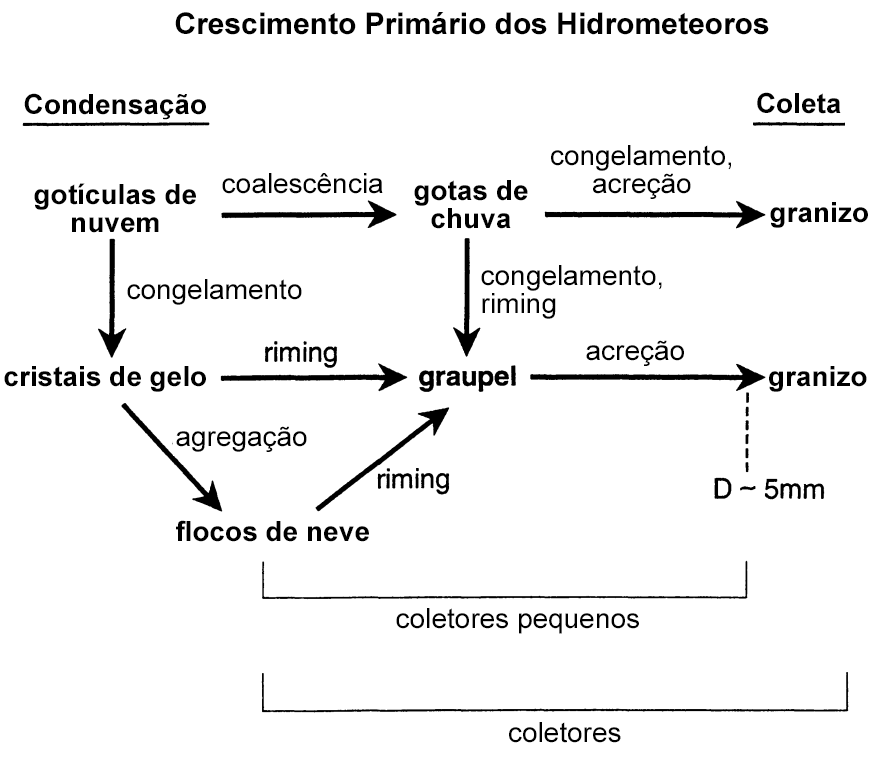
\includegraphics[width=0.7\columnwidth]{figs/growth_knight_ptbr.png}
		\legend{Fonte: Adaptado de \citeonline{Knight2001}.}
	\end{center}
\end{figure}

Dentro da região de fase mista da nuvem, a colisão entre hidrometeoros contribui não só para o crescimento mas também para a troca de cargas entre eles através da transferência de massa. Considerando o momento de dipolo permanente da água, que expõe íons negativos na camada quase-líquida das partículas, a colisão entre dois hidrometeoros transfere íons negativos do hidrometeoro com maior camada para o com menor camada, deixando assim o primeiro positivamente carregado e o segundo negativamente carregado \cite{Baker1987, Baker1994b}. Com a atuação da corrente ascendente, a distribuição de hidrometeoros carregados geram centros de cargas bem definidos dentro da nuvem, e é na interface entre centros de cargas opostas que ocorre a quebra de rigidez dielétrica que origina uma descarga elétrica. Assim, esse mecanismo, chamado de carregamento não-indutivo, é fundamental para a eletrificação de tempestades \cite{Saunders2008}.

A espessura da camada quase-líquida de um hidrometeoro na região de fase mista depende do tipo e tamanho do hidrometeoro e também de fatores externos como conteúdo de água líquida e temperatura. A \autoref{takahashi} mostra o resultado obtido por \citeonline{Takahashi1978} através de medidas em laboratório: após a colisão com cristais de gelo, o graupel fica carregado positivamente independentemente do conteúdo de água líquida em temperaturas mais altas que $-10^{\circ}C$; em temperaturas mais baixas, o graupel fica positivamente carregado quando o conteúdo de água líquida é muito alto (acima de $2\:gm^{-3}$) ou muito baixo (abaixo de $0,2\:gm^{-3}$), enquanto que fica negativamente carregado quando o conteúdo de água líquida está entre $0,2\:gm^{-3}$ e $2\:gm^{-3}$. \citeonline{Williams1991} indicam que o regime de crescimento do graupel/granizo também muda com o conteúdo de água líquida e temperatura (linhas pontilhadas da \autoref{takahashi}): o regime de crescimento é molhado quando o conteúdo de água líquida é muito alto e/ou a temperatura é próxima de $0^{\circ}C$, seco por deposição quando o conteúdo de água líquida e/ou a temperatura são muito baixos e seco por sublimação entre as duas porções anteriores. É importante ressaltar que não há um consenso em relação à esses valores, já que outros estudos feitos em laboratório \cite{Jayaratne1983, Pereyra2000, Saunders2006} não encontraram os mesmos resultados. \citeonline{Emersic2010}, por exemplo, mostraram que o sinal de carregamento do graupel e temperaturas associadas em experimentos de laboratório é dependente da configuração experimental da câmera de nuvem, essencialmente do modo de nucleação dos cristais de gelo, isto é, crescer juntamente com ou separadamente da nuvem de gotículas superresfriadas, o que controla a espessura da camada quase-líquida e a taxa relativa de crescimento por difusão de vapor. Os fatores externos descritos aqui são altamente influenciados pela intensidade da corrente ascendente, já que correntes ascendentes mais intensas promovem maior transporte de água líquida para a região de fase mista da nuvem. 

\begin{figure}[htb]
	\begin{center}
		\caption{Carga adquirida pelo graupel/granizo após a colisão com cristais de gelo em função do conteúdo de água líquida e temperatura. As linhas pontilhadas delimitam os regimes de crescimento molhado (porção superior), crescimento seco por sublimação (porção central) e crescimento seco por deposição (porção inferior).} 
		\label{takahashi}
		%		\setcaptionmargin{1cm}
		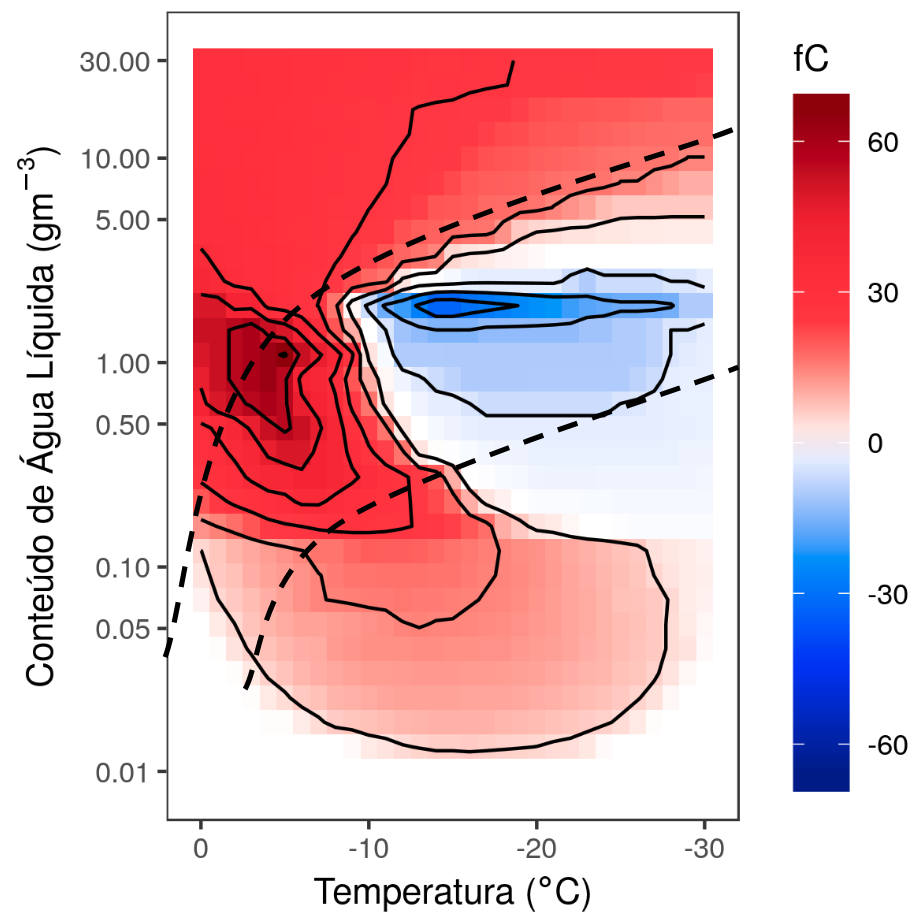
\includegraphics[width=0.6\columnwidth]{figs/takahashi_williams_ptbr.png}
		\legend{Fonte: Adaptado de \citeonline{Takahashi1978} e \citeonline{Williams1991}.}
	\end{center}
\end{figure}

Simultaneamente à troca de cargas entre graupel/granizo e cristais de gelo, a corrente ascendente transporta e concentra esses hidrometeoros de acordo com a velocidade terminal de cada um: graupel e granizo tendem a entrar em equilíbrio com a corrente ascendente ou descer para fora da região de fase mista, enquanto que os cristais de gelo são transportados para a porção superior ou acima da região de fase mista. Assim, centros de cargas elétricas são formados dentro da nuvem, e a distribuição desses centros depende da complexidade da cinemática da nuvem. Uma descrição simplificada de uma estrutura de cargas na forma de um dipolo foi feita por \citeonline{Wilson1921}, \citeonline{Simpson1937} e \citeonline{Simpson1941}, mas \citeonline{Williams1989} consolidou a estrutura de cargas tripolar como sendo a mais comumente encontrada na região de corrente ascendente em tempestades ao revisar diversos experimentos em laboratório e \textit{in-situ}. Essa hipótese considera que o regime de crescimento preferencial do graupel/granizo é seco por deposição, o que significa que eles ficam negativamente carregados (região de carregamento negativo na \autoref{takahashi}); com a atuação da corrente ascendente, um centro de cargas negativas principal é formado na região de fase mista, com dois centros de cargas positivas acima (com cristais de gelo) e abaixo (com hidrometeoros em tamanhos precipitáveis) dessa região, produzindo mais raios nuvem-solo (\textit{cloud-to-ground}, CG) de polaridade negativa. Porém, diversos estudos \textit{in-situ}  \cite{Macgorman1994, Carey1995a, Lyons1998, Carey2003e, Carey2007, Pineda2016} mostram que tempestades severas produzem muito mais raios CG de polaridade positiva; dentre as hipóteses que procuram explicar esse fenômeno está a estrutura de tripolo invertido: a corrente ascendente mais intensa aumenta o conteúdo de água líquida na região de fase mista, promovendo o crescimento molhado e carregamento positivo do graupel/granizo (região de carregamento positivo em alto conteúdo de água líquida na \autoref{takahashi}); assim, a estrutura simplificada é formada por um centro de cargas positivas na região de fase mista e dois centros de cargas negativas acima e abaixo dessa região, gerando maior quantidade de raios CG positivos. Além disso, tempestades severas também podem promover a formação de granizos gigantes através de ciclos de movimentos descendentes e ascendentes no flanco direito do núcleo de corrente ascendente \cite{Knight1970, Knight2001c, Knight2005} e apresentar picos de atividade elétrica antes da ocorrência de tempo severo (\textit{lightning jump}, salto de raios) \cite{Goodman1988, Williams1999, Schultz2009a, Gatlin2010, Schultz2011}.

\section{Medindo Características de Tempestades de Granizo}

O principal fenômeno que separa tempestades de granizo de tempestades não-severas é a queda de granizo na superfície, que pode causar danos quando o granizo possui tamanho grande ou gigante (diâmetro maior que $19\:mm$). Por esse motivo, medidas de granizo são importantes para caracterizar e posteriormente prever a ocorrência e potencial destrutivo desse tipo de tempestade severa. Medidas \textit{in-situ} usando \textit{hailpads} - placas de isopor especial fixadas na superfície ou em suportes a uma certa altura que, através das cavidades formadas após o impacto dos granizos nas placas, geram distribuições de tamanho de granizo \cite{Schleusener1960a, Decker1961} - fornecem informações precisas sobre esse fenômeno em uma escala local, similar à representatividade de um pluviômetro na medida de precipitação. Diversas redes de \textit{hailpads} instaladas em países da Europa \cite{Dessens1998, Svabik1989, Giaiotti2003, Pocakal2009, Berthet2011} e na Argentina \cite{Sanchez2009} permitiram uma caracterização das tempestades de granizo nessas regiões, inclusive em longos períodos \cite{Berthet2013}. No Brasil, uma rede foi instalada no estado de Santa Catarina, em uma região rural, para estimar a eficiência de um sistema "anti-granizo" \cite{Iliine2010}. Diversos trabalhos utilizam medidas de \textit{hailpads} como base de comparação com estimativas por sensoriamento remoto, principalmente radares meteorológicos \cite{Waldvogel1978a, Schmid1992, Sanchez2013}.

Uma grandeza ligada à distribuição de tamanho de granizo que estima o potencial destrutivo de uma tempestade de granizo é a energia cinética, equivalente ao trabalho mecânico que a superfície sofre ao ser atingida pelo granizo. \citeonline{Changnon1971} e \citeonline{Morgan1976} mostraram que essa grandeza possui maior relação com danos em plantações do que o tamanho ou quantidade de granizo. Além disso, a energia cinética do granizo pode ser estimada mais facilmente por radares já que a refletividade medida por eles tem a mesma ordem de grandeza do diâmetro do granizo \cite{Waldvogel1978a}, o que permite, por exemplo, que diversos trabalhos relacionem diretamente a energia cinética com danos em edificações \cite{Hohl2002, Schuster2006}.

\section{Tempestades de Granizo na América do Sul}

Diferentemente de tempestades em latitudes médias, tempestades tropicais raramente são intensas o suficiente para gerar queda de granizo ou graupel no solo, com exceção da África Central \cite{Court1982, Hand2011, Cecil2012a}. Como mostrado na \autoref{sinotica_barnes}, a porção central e norte da América do Sul não apresenta condições sinóticas que favoreçam a formação de convecção organizada e sistemas convectivos de mesoescala (por ser um ambiente barotrópico, com baixos gradientes de temperatura), apenas tempestades isoladas principalmente durante o verão (Figura\autoref{sinotica_jan}); essas tempestades costumam ter pouco tempo de vida e correntes ascendentes insuficientes para transportar grandes quantidades de água líquida para a região de fase mista e promover o crescimento de granizo. Já mais ao sul, tempestades de granizo destrutivas têm sido relatadas na Argentina subtropical e na região sul do Brasil \cite{Court1982, Martins2017}; satélite, modelagem e climatologias mostram que essa área pode chegar a $\ang{15}S$ de latitude \cite{Hand2011, Cecil2012a, Albrecht2016}.

\begin{figure}[htb]
	\begin{center}
		\caption{Esquema com as características de escala planetária e sinótica primárias encontradas na superfície no Atlântico Tropical em janeiro (a) e julho (b).} 
		\label{sinotica_barnes}
		\subfloat[]{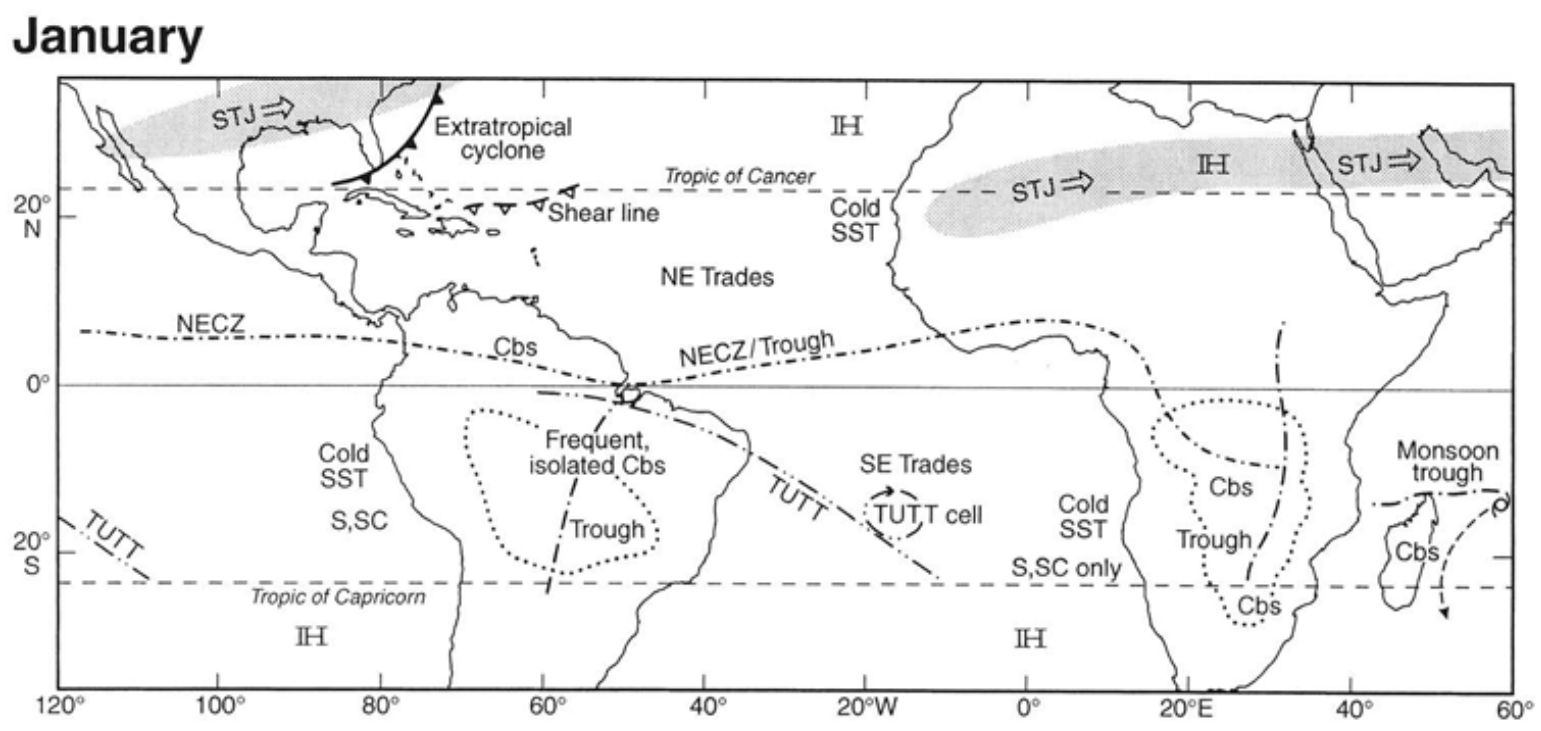
\includegraphics[width=0.8\columnwidth]{figs/barnes_synoptic_jan.png}
			\label{sinotica_jan}} \\
		\subfloat[]{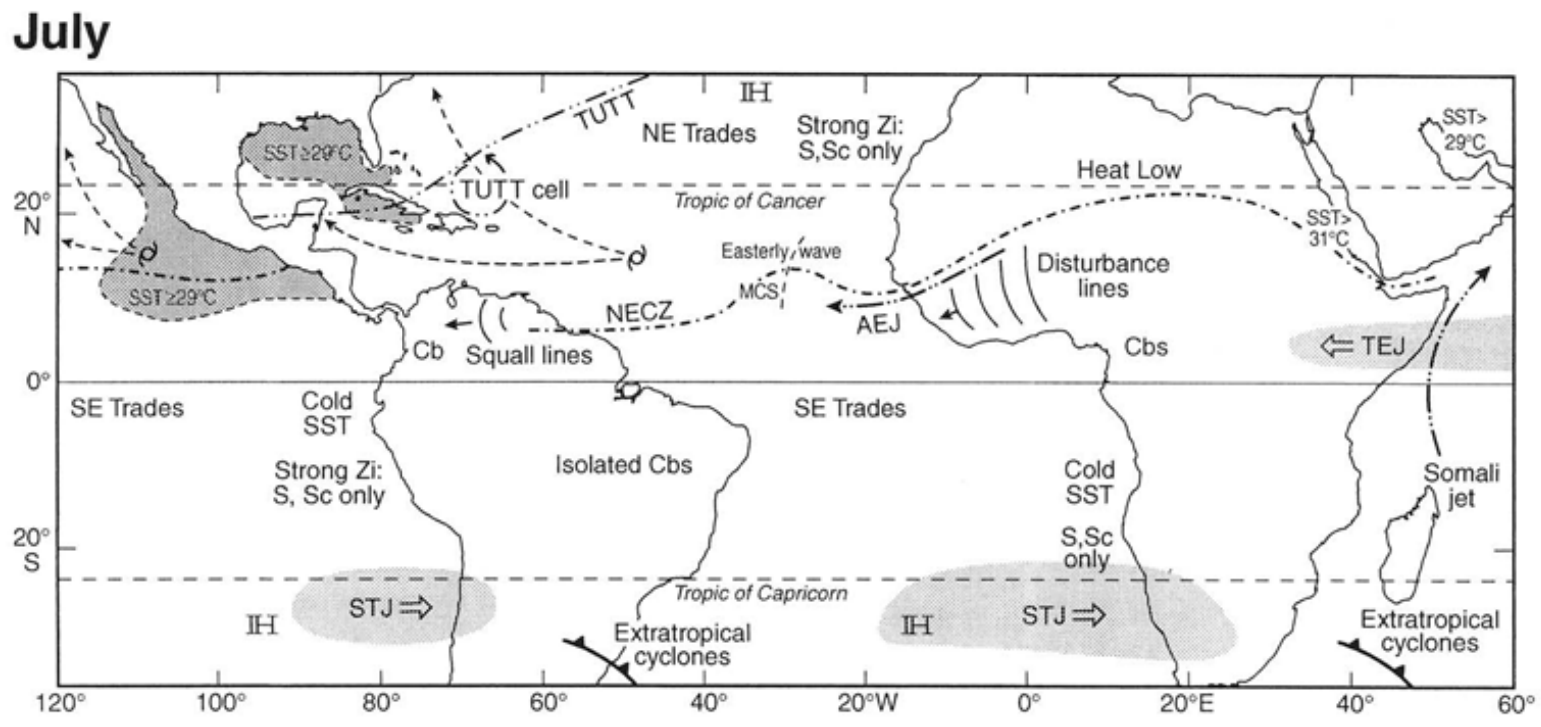
\includegraphics[width=0.8\columnwidth]{figs/barnes_synoptic_jul.png}
			\label{sinotica_jul}} \\
		\legend{Fonte: \citeonline{Barnes2001}.}
	\end{center}
\end{figure}

A \autoref{climatologia_granizo} mostra uma climatologia de tempestades de granizo severas (ou seja, com queda de granizos grandes ou gigantes) no sudeste da América do Sul usando uma série temporal de 8 anos de dados do sensor passivo em microondas AMSR-E (\textit{Advanced Microwave Scanning Radiometer for Earth Observing System}, Radiômetro Avançado de Escaneamento em Microondas para o Sistema de Observação Terrestre) a bordo do satélite de órbita sincronizada com o Sol \textit{Aqua}. O pico de frequência de tempestades de granizo está centrado no norte da Argentina, se estendendo ao Paraguai, Uruguai e partes de Brasil e Bolívia \cite{Cecil2012a}. \citeonline{Barnes2001} (em sua Figura 10.31) mostra que o ciclo anual de eventos de granizo no Brasil (entre 18 e $\ang{22}S$) é sazonal, com maior frequência na primavera e verão. \citeonline{Sperling2018} também mostra maior frequência de granizo durante a primavera considerando eventos no sul do Brasil, que são produzidos por tempestades isoladas de grande extensão vertical antes de se juntarem a sistemas convectivos de mesoescala formados ao longo do jato sul-americano de baixos níveis em situações pré-frontais. Essas tempestades são formadas por pequenas células convectivas explosivas que rapidamente (até 30 minutos) desenvolvem uma região de fase mista com refletividade acima de $50\:dBZ$ até $18\:km$ de altura; entre 10 e 20 minutos depois do crescimento explosivo das células e aumento da massa de gelo, há um distinto salto na taxa de raios totais, produzindo granizo com mais de $6\:cm$ de diâmetro observado no solo. No sudeste do Brasil, incluindo a região de estudo desta dissertação, a frequência e tamanho do granizo são menores que no sul do Brasil, mas também produzidos por pequenas células convectivas em situações pré-frontais \cite{Puig2017}. 

\begin{figure}[htb]
	\begin{center}
		\caption{Climatologia anual de granizo a partir do sensor AMSR-E para o sudeste da América do Sul. Os contornos em cinza indicam a elevação, com intervalos de $1\:km$.} 
		\label{climatologia_granizo}
		%		\setcaptionmargin{1cm}
		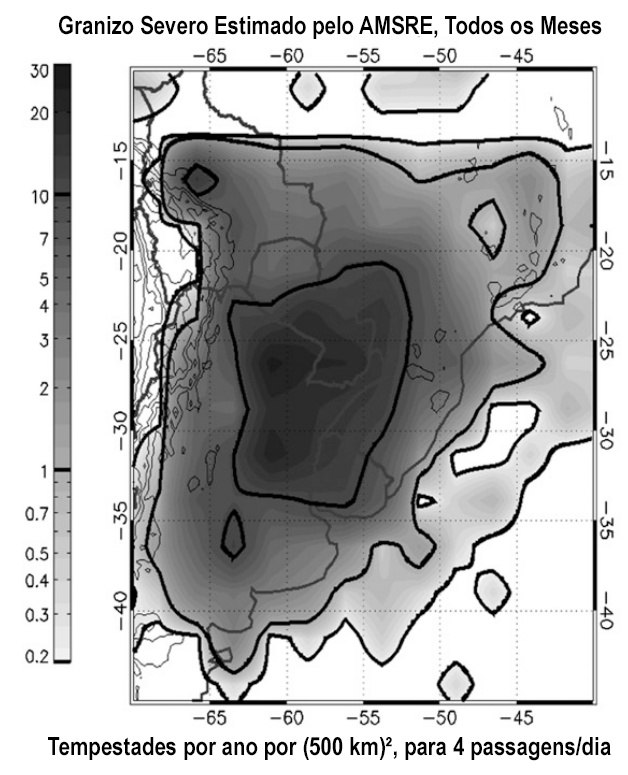
\includegraphics[width=0.5\columnwidth]{figs/cecil_severehail_ptbr.png}
		\legend{Fonte: Adaptado de \citeonline{Cecil2012a}.}
	\end{center}
\end{figure}

\section{Usando Radares Meteorológicos para Estudar a Cinemática das Tempestades}

Radares Doppler possuem a capacidade de medir a velocidade dos alvos que estão em seu volume observado, gerando essa importante informação sobre as nuvens com alta resolução espacial. A partir da velocidade desses alvos, é possível derivar não só o deslocamento da nuvem em si como também o escoamento dentro da nuvem, inferindo assim as propriedades cinemáticas da nuvem e sua importância para o ciclo de vida. É possível extrair informações relacionadas ao campo de vento a partir da recuperação das componentes do vento com um  (display de velocidade-azimute (VAD, \textit{velocity-azimuth display}); para mais informações, ver seção 11.5 de \citeonline{Rauber2018}) ou mais radares (Dual ou Multi-Doppler; gera um campo tridimensional do vento). Para tempestades de granizo, por exemplo, \citeonline{morgan1986thunderstorm} afirmam que técnicas Dual ou Multi-Doppler oferecem a descrição mais realista do ambiente relacionado ao granizo, pois permite observar efeitos de advecção com alto grau de detalhamento.

Desde a primeira formulação do método de recuperação de vento tridimensional \cite{Armijo1969}, diversos trabalhos usaram este método para entender a cinemática de tempestades. Estudos pioneiros descrevem a estrutura de tempestades severas \cite{Brandes1977, Ray1980}, frentes de rajada \cite{Weaver1982}, tempestades não-severas usando Multi-Doppler \cite{Ray1978} e microexplosões \cite{Wilson1984} nos Estados Unidos, além do estudo de uma linha de instabilidade tropical no oeste da África \cite{Chong1987}. O desenvolvimento de métodos e ferramentas mais sofisticadas permitiu estudos detalhados de tempestades que causaram grandes volumes de precipitação \cite{Petersen1999a, Calhoun2013} e supercélulas \cite{Potvin2012a, Potvin2012b}, incluindo um caso com sucessivas tornadogêneses \cite{Wurman2007}; \citeonline{Hubbert1998a} usou o método Dual-Doppler para auxiliar na identificação dos processos microfísicos associados à assinaturas nas variáveis polarimétricas em um caso com queda de granizos gigantes. Outros estudos buscaram estudar a estrutura de diversos tipos de tempestades para descrever as principais diferenças na cinemática convectiva entre tempestades severas e não-severas \cite{Lang2002, Deierling2008}. No Brasil, o experimento TRMM-LBA (\textit{Tropical Rainfall Measuring Mission Large Scale Biosphere-Atmosphere Experiment in Amazonia}, Experimento de Larga Escala Biosfera-Atmosfera na Amazônia da Missão de Medidas de Precipitação Tropical) gerou diversos estudos da cinemática de tempestades tropicais na Amazônia durante o período chuvoso, mostrando que as tempestades que se desenvolvem em um escoamento de leste em baixos níveis apresentam extensão vertical maior e correntes ascendentes mais intensas comparando com as que se desenvolvem em um escoamento de oeste \cite{Rutledge2000, Cifelli2002b, Cifelli2004a}.

A base teórica do método de recuperação de vento tridimensional consiste em determinar 4 componentes da velocidade do vento em coordenadas cartesianas: $u$, $v$, $w$ e $w_t$, onde as três primeiras são as componentes da velocidade nas coordenadas $x$, $y$ e $z$ e $w_t$ é a velocidade terminal da precipitação \cite{Rinehart1997}. Dois radares Doppler vendo a mesma tempestade de ângulos diferentes fornecem duas medidas distintas de velocidade radial ($v_{r_1}$ e $v_{r_2}$), como mostra a \autoref{doviak_sistema}, e $w_t$ pode ser estimada em função da refletividade (usando uma distribuição de Marshall-Palmer, por exemplo). Assim, $u$ e $v$ podem ser descritos como:

\begin{figure}[htb]
	\begin{center}
		\caption{Sistema de coordenadas cilíndricas usado para análise Dual-Doppler de dados de radar. Os radares estão localizados nos pontos 1 e 2 e $a_r$, $a_s$ e $a_\alpha$ são as normais unitárias definindo a direção das três componentes ortogonais da velocidade. O eixo cilíndrico está ao longo da linha conectando os radares (separados por uma distância $2d$) e $r$ é a distância do eixo ao dado pontual.} 
		\label{doviak_sistema}
		%		\setcaptionmargin{1cm}
		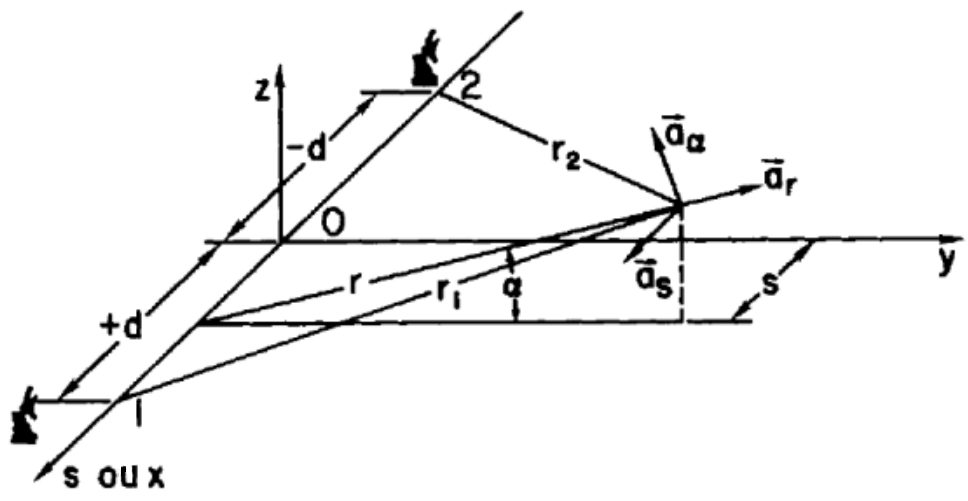
\includegraphics[width=0.8\columnwidth]{figs/system_doviak_ptbr.png}
		\legend{Fonte: Adaptado de \citeonline{Doviak1993}.}
	\end{center}
\end{figure}

\begin{equation}
u=\frac{1}{\sin{(\theta_1 - \theta_2)}}\left(\frac{v_{r_1}\cos{\theta_2}}{\sin{\alpha_1}}-\frac{v_{r_2}\cos{\theta_2}}{\sin{\alpha_2}}\right)
\end{equation}

\begin{equation}
v=\frac{1}{\sin{(\theta_1 - \theta_2)}}\left(\frac{v_{r_2}\cos{\theta_1}}{\sin{\alpha_2}}-\frac{v_{r_1}\cos{\theta_1}}{\sin{\alpha_1}}\right)
\end{equation}

\noindent
onde $\theta_1$ e $\theta_2$ são os ângulos azimutais dos radares $1$ e $2$, respectivamente, e $\alpha_1$ e $\alpha_2$ são os ângulos de elevação dos mesmos.

Para calcular a componente vertical da velocidade, a equação de continuidade de massa é usada, assumindo como condições de contorno que a velocidade na superfície e no topo da tempestade são nulas, ou seja:

\begin{equation} 
\label{continuidade_massa}
\frac{\partial(\rho w)}{\partial z}=-\rho\left(\frac{\partial u}{\partial x} + \frac{\partial v}{\partial y}\right)
\end{equation}

\begin{equation}
w=w_T-w_t
\end{equation}

\noindent
onde $\rho$ é a densidade do ar atmosférico e $w_T$ é a velocidade vertical total. Quando três radares são usados, é possível calcular o campo tridimensional sem usar a \autoref{continuidade_massa}.

Ao combinar radares Doppler para a recuperação do vento, a área de cobertura e erros característicos (altura do feixe e resolução espacial) devem ser considerados \cite{Dolan2007}. Se a distância da linha de base entre os dois radares for longa, a área de cobertura será maior mas a resolução espacial será prejudicada. Além disso, se o ângulo de cruzamento do feixe é pequeno (mais paralelo), as duas medidas serão mais similares e as variâncias dos erros de velocidade nas estimativas Dual-Doppler - $\sigma_u^2$ e $\sigma_v^2$ - serão menores. De acordo com \citeonline{Davies-Jones1979}, $\sigma_u^2$ e $\sigma_v^2$ estão relacionadas com as variâncias dos erros de velocidade Doppler de cada radar, $\sigma_1^2$ e $\sigma_2^2$, da seguinte forma:

\begin{equation}
\frac{\sigma_u^2+ \sigma_v^2}{\sigma_1^2 + \sigma_2^2}=\csc^2{\beta}
\end{equation}

\noindent
onde $\beta$ é o ângulo de cruzamento do feixe entre os dois radares. Para $\beta\:<\:\ang{30}$, $\sigma_u^2$ e $\sigma_v^2$ crescem rapidamente \cite{Doviak1976, Davies-Jones1979, Doviak1993}.

A \autoref{doppler_theory_lobes} mostra teoricamente as áreas aceitáveis para estimativa de velocidade do vento considerando dois valores de $\beta$: $\ang{30}$ e $\ang{45}$. Quanto maior o valor de $\beta$, melhor é a estimativa Dual-Doppler, mas menor será a área de cobertura dessa estimativa.

\begin{figure}[htb]
	\begin{center}
		\caption{Ângulos teóricos de cruzamento do feixe com Dual-Doppler de \ang{45} (melhores dados de vento) e \ang{30} (dados de vento aceitáveis) para um par de radares Doppler.} 
		\label{doppler_theory_lobes}
		%		\setcaptionmargin{1cm}
		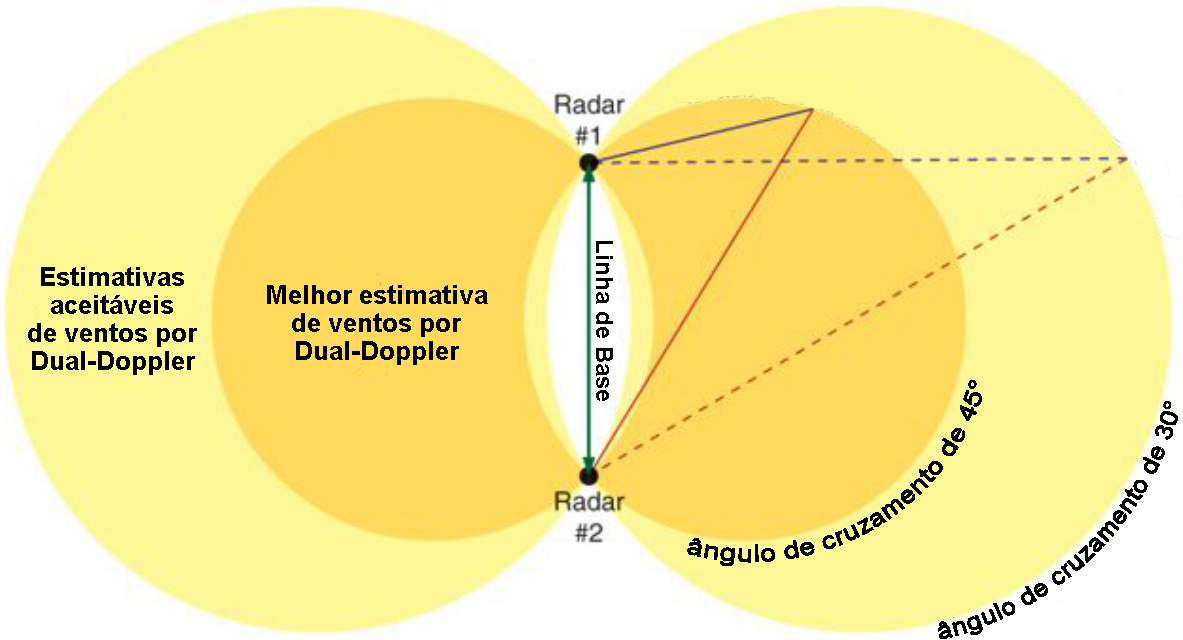
\includegraphics[width=\columnwidth]{figs/lobes_eastin_ptbr.png}
		\legend{Fonte: Adaptado do original fornecido pelo Dr. Matthew D. Eastin, UNC.}
	\end{center}
\end{figure}



% Dados e Métodos
\chapter{Material e Métodos}\label{database}

A partir da base de dados do Projeto SOS-CHUVA, cinco casos foram selecionados, onde houve queda de granizo medida pela rede de hailpads (\autoref{hailpads}). A \autoref{tabela_casos} mostra uma breve descrição de cada caso.

\begin{table}[htb]
	\IBGEtab{%
		\caption{Descrição dos casos selecionados para análise.}%
		\label{tabela_casos}
	}{%
		\begin{tabularx}{\textwidth}{cYYY}
			\toprule
			Caso & Descrição & Regiões Afetadas & Tipo de Severidade \\
			\midrule
			2016-12-25 & Condições instáveis na região levou à formação de diversos sistemas convectivos & Campinas, Vale do Paraíba, São Carlos & Rajadas de vento, granizo \\
			\midrule 
			2017-01-31 & Linha de Instabilidade & Sorocaba, Itu, Araraquara & Granizo \\
			\midrule 
			2017-03-14 & Chuva forte e queda de granizo entre Campinas e Indaiatuba e em Jacareí & Campinas, Indaiatuba, Jacareí & Granizo \\
			\midrule 
			2017-11-15 & Condições termodinâmicas favoráveis levaram à formação de sistemas convectivos concentrados no centro do estado de SP & Indaiatuba, Bebedouro & Granizo \\
			\midrule 
			2017-11-16 & Condições termodinâmicas favoráveis e um cavado em médios níveis favoreceram a formação de sistemas convectivos & Lorena, Ribeirão Preto, Campinas, São Paulo, Itapeva & Rajadas de vento, granizo \\
			\bottomrule
		\end{tabularx}%
	}{%
		\fonte{Adaptado de https://topicssoschuva.blogspot.com.br/2017/03/summary-of-case-studies.html.}%
	}
\end{table}


\section{Rede de Detecção de Granizo}\label{hailpads}

Dentro do Projeto SOS-CHUVA, uma rede de detecção de granizo foi instalada na Região Metropolitana de Campinas, dentro da cobertura do radar meteorológico Banda-X instalado na UNICAMP (XPOL). Como mostrado na Figura\autoref{rede_hailpads}, a rede foi composta por 24 localidades, com maior densidade de pontos nas cidades de Campinas e Indaiatuba. O instrumento, chamado de hailpad, é composto por uma placa de isopor usado para isolamento coberta por uma folha de alumínio e fixada em um suporte de ferro aproximadamente 1,5 m acima da superfície. Na Figura\autoref{hailpad_indaiatuba} é possível observar uma placa instalada em Indaiatuba.

\begin{figure}[htb]
	\begin{center}
		\caption{(a) Rede de hailpads instalada na Região Metropolitana de Campinas com a localização e cobertura de 80 km do radar XPOL. (b) Hailpad instalado na cidade de Indaiatuba, na localização indicada com a seta em (a)} 
		\label{overview_hailpads}
		\subfloat[]{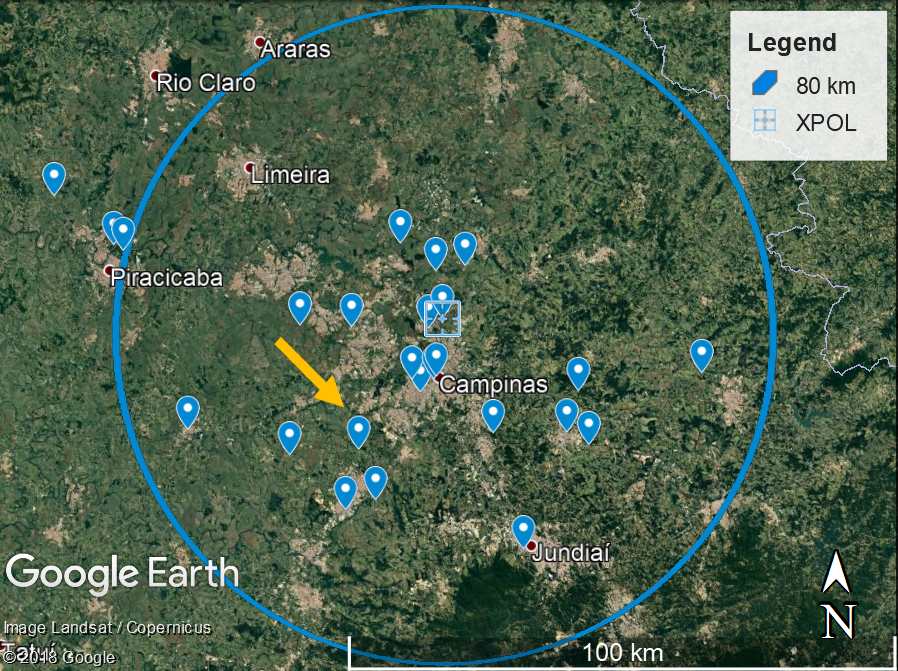
\includegraphics[width=0.75\columnwidth]{figs/hailpad_network.png}
			\label{rede_hailpads}}
		\ \
		\subfloat[]{\includegraphics[width=0.158\columnwidth]{figs/hailpad.png}
			\label{hailpad_indaiatuba}}\\
		\legend{Fonte: Produzido pela autora.}
	\end{center}
\end{figure}

Os casos descritos na \autoref{tabela_casos} foram selecionados com base nos registros dos hailpads dentro da rede. A \autoref{tabela_hailpads} mostra a localização das placas e os grupos que mediram a distribuição de tamanho de granizo, sendo eles: Departamento de Ciências Atmosféricas (DCA/IAG-USP) e Laboratório de Instrumentação Meteorológica (LIM/CPTEC-INPE). Não houve registro da localização exata da placa C004. 

\begin{table}[htb]
	\IBGEtab{%
		\caption{Descrição dos hailpads coletados para cada caso}%
		\label{tabela_hailpads}
	}{%
		\begin{tabularx}{\textwidth}{YYYY}
			\toprule
			Data do evento & Código do hailpad coletado & Localização & Medido por \\
			\midrule 
			2016-12-25 & C002 & Campinas & IAG, LIM \\
			\midrule 
			2017-01-31 & C003 & Campinas & IAG, LIM \\ 
			 & C004 & Arredores de Campinas & IAG, LIM \\
			\midrule 
			2017-03-14 & C001 & Cosmópolis & IAG \\ 
			& R002 & Indaiatuba & IAG \\
			\midrule 
			2017-11-15 & R004 & Indaiatuba & IAG \\
			\midrule 
			2017-11-16 & R038 & Campinas & IAG \\
			\bottomrule
		\end{tabularx}%
	}{%
		\fonte{Produzido pela autora.}%
	}
\end{table}

A partir de um hailpad é possível derivar diversas grandezas relacionadas à tempestade que gerou a queda de granizo. A principal delas é a distribuição de tamanho de granizo, medindo as cavidades na placa sensibilizada (\autoref{hailpad_exemplo}). Essa grandeza foi obtida através de uma série de medições manuais dos diâmetros das cavidades com um paquímetro e ajustando os dados com a curva de calibração desse tipo de isopor, realizada pelo LIM e exibida na \autoref{calibracao_hailpad}. Com essa distribuição, pode-se calcular a energia cinética do granizo (quando diversas placas mediram um mesmo evento) ou do hailpad (quando poucas ou uma única placa mediram um evento). Ambas grandezas são equivalentes ao trabalho mecânico sofrido pela superfície onde caiu o granizo, indicando então o dano causado por ele na superfície.

\begin{figure}[htb]
	\begin{center}
		\caption{Placa R004 sensibilizada no sítio (a) e sem a cobertura de alumínio (b)} 
		\label{hailpad_exemplo}
		\subfloat[]{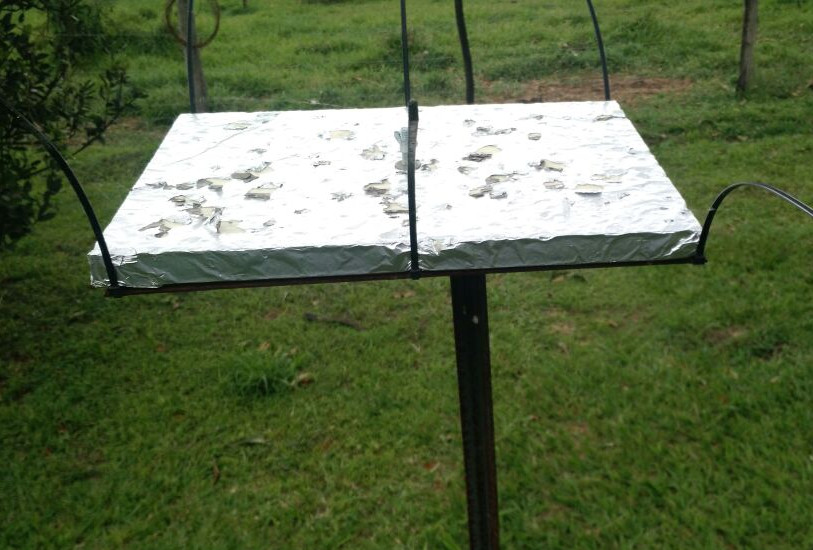
\includegraphics[width=0.4\columnwidth]{figs/hailpad_site.jpg}
			\label{hailpad_sensibilizado}}
		\quad
		\subfloat[]{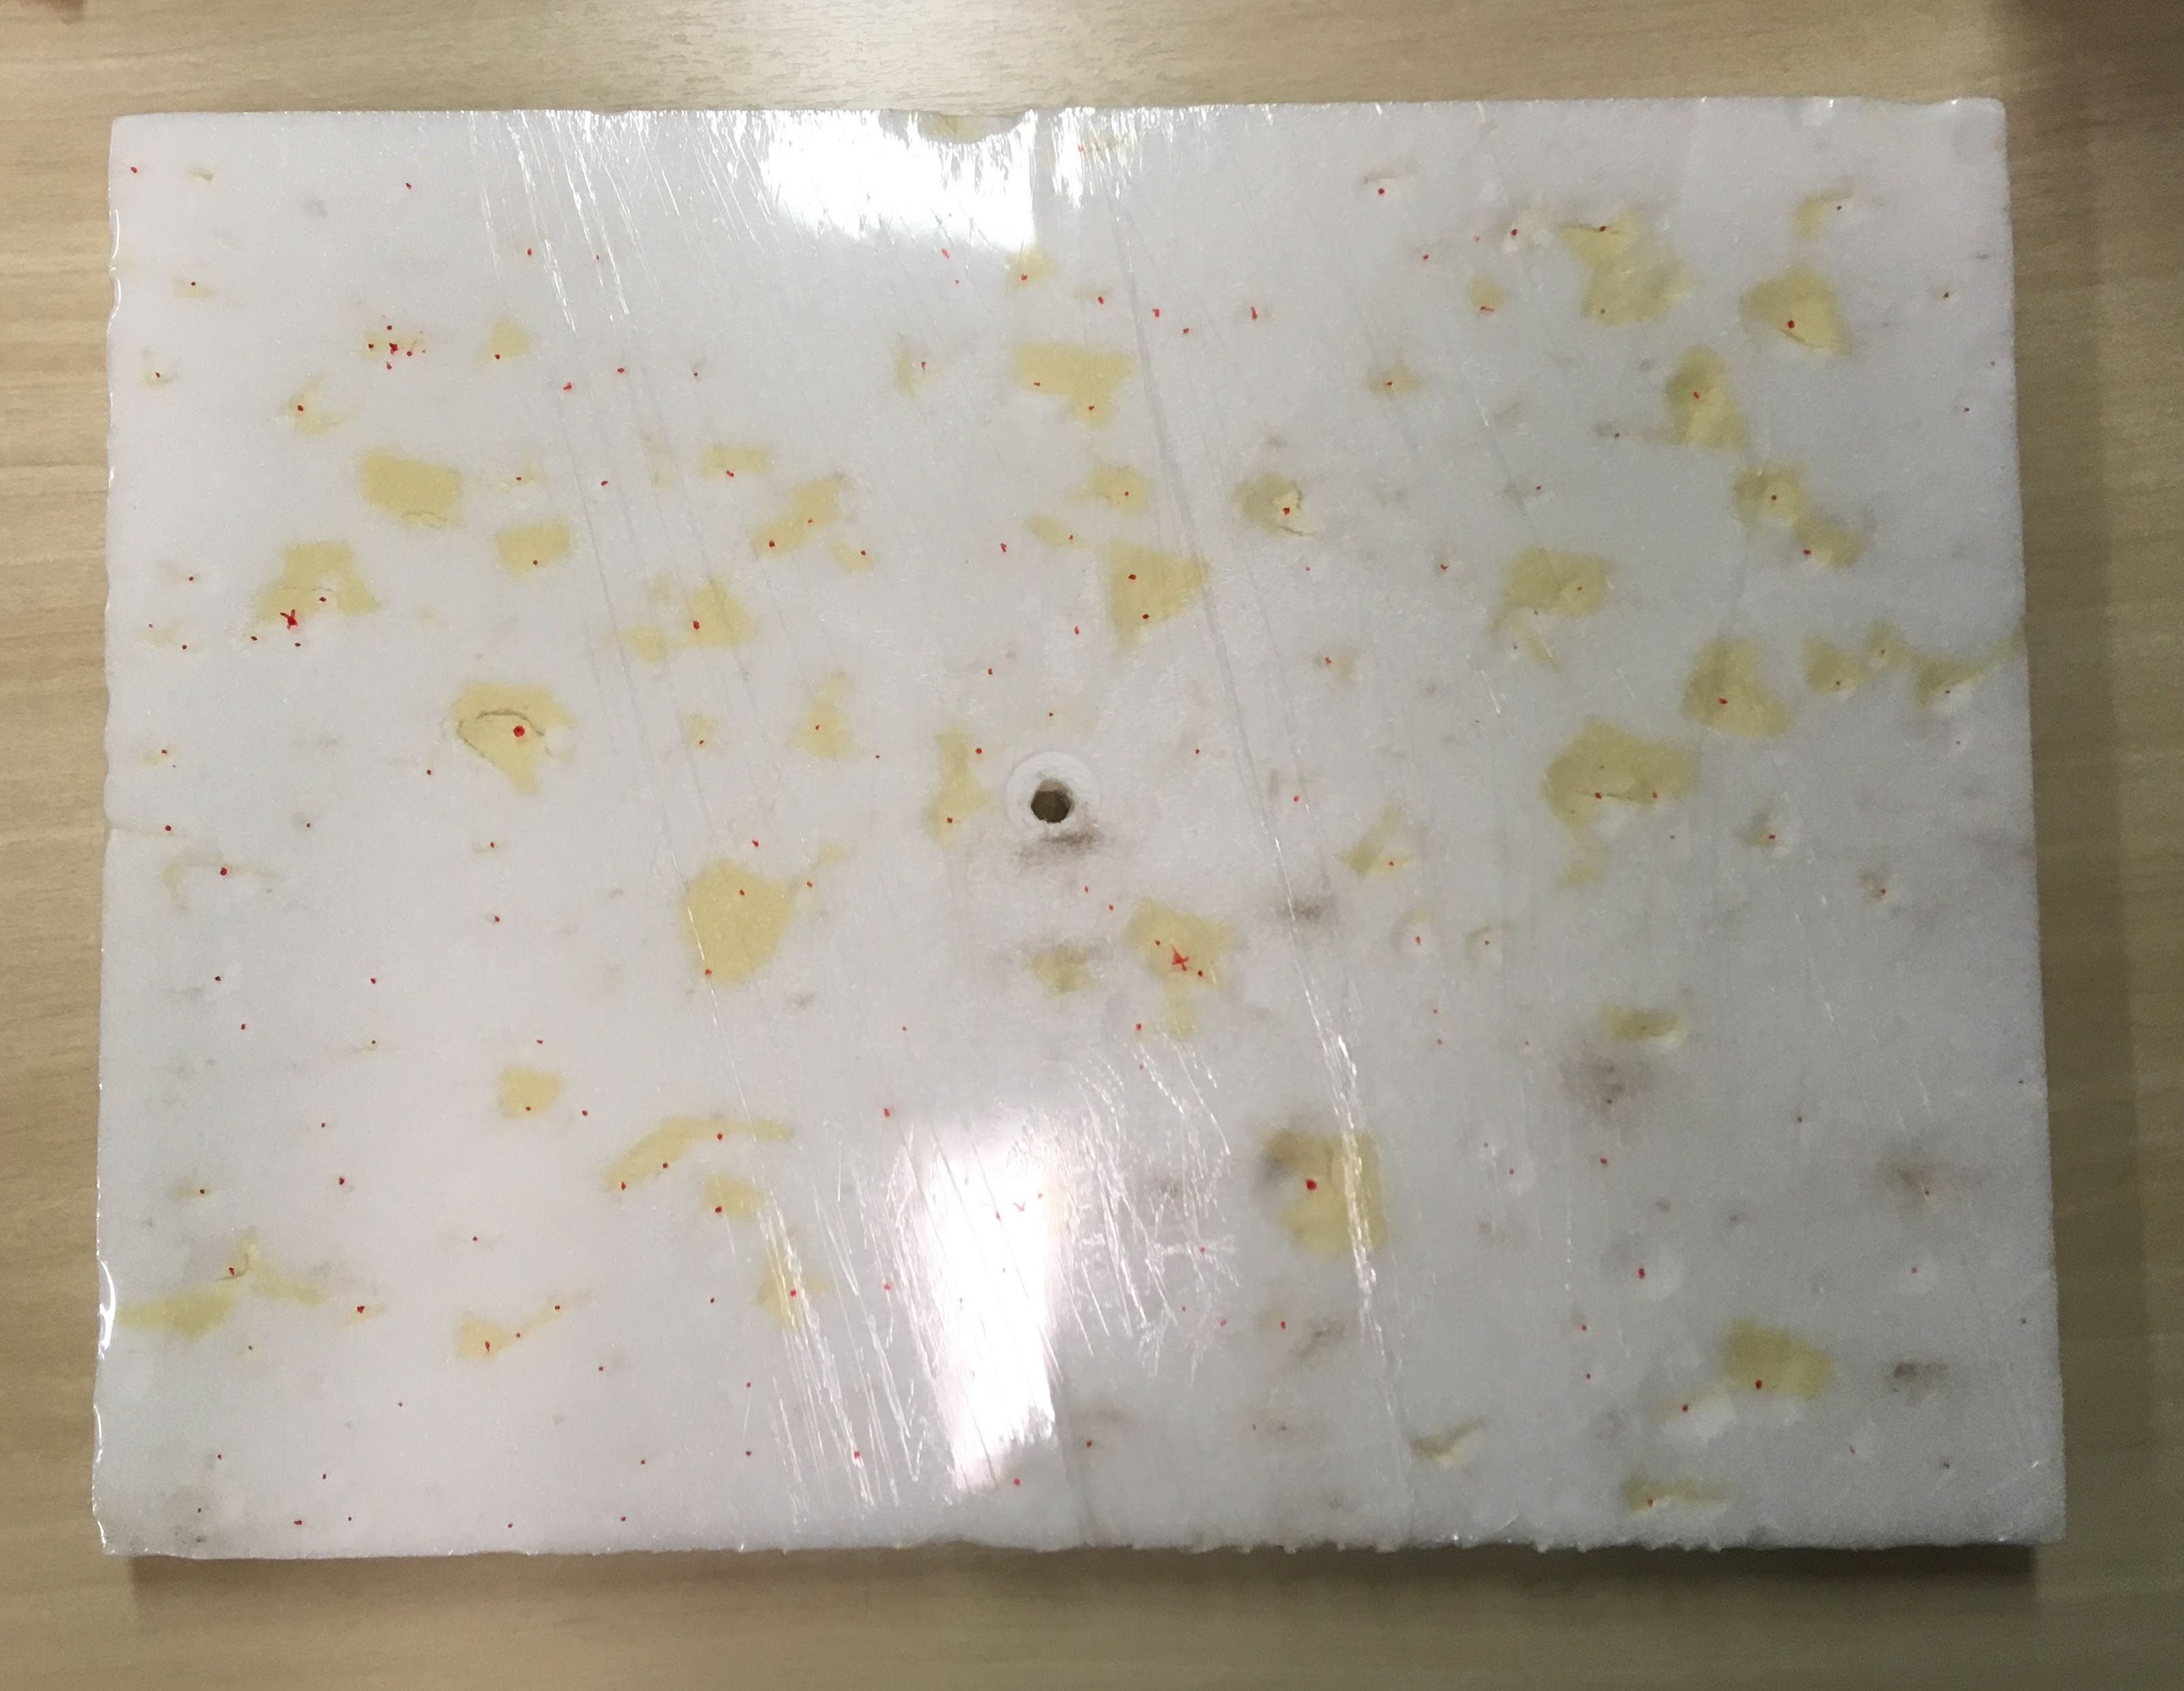
\includegraphics[width=0.355\columnwidth]{figs/hailpad_used.JPG}
			\label{hailpad_semaluminio}}\\
		\legend{Fonte: A autora.}
	\end{center}
\end{figure}

\begin{figure}[htb]
	\begin{center}
		\caption{Curva de calibração do hailpad obtida pelo LIM/CPTEC-INPE} 
		\label{calibracao_hailpad}
%		\setcaptionmargin{1cm}
		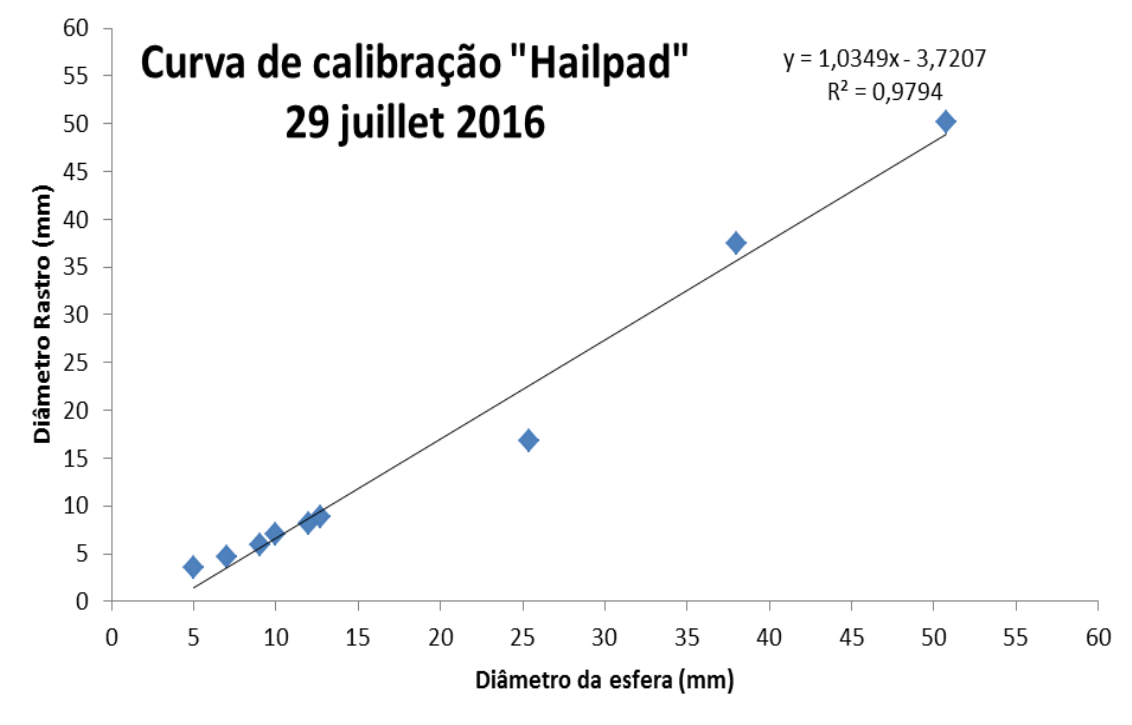
\includegraphics[width=0.7\columnwidth]{figs/calibracao_hailpad.png}
		\legend{Fonte: \citeonline{ThomazJunior2015a}.}
	\end{center}
\end{figure}

Como houve no máximo 2 placas sensibilizadas em todos os casos, calculou-se a energia cinética do hailpad $E_t\:(Jm^{-2})$, definida por \citeonline{Mezeix1981} como:

\begin{equation} \label{mezeix}
	E_t = 4,58\:e^{-6} \sum_{i=1}^{k} n_i d_i^4
\end{equation}

\noindent
sendo $n_i$ a quantidade de pontos por $m^2$ em um dado diâmetro médio $d_i\:(mm)$ de um intervalo $\Delta d$. $k$ é o numero de intervalos, igual a 9 nesse caso já que $\Delta d$ variou entre $2$ e $22\:\:mm$ com espaçamento de $1\:mm$. Foram consideradas incertezas nas medidas propagando o desvio-padrão da distribuição média entre as diferentes medidas de uma mesma placa.

Com os valores de diâmetro do granizo e energia cinética do hailpad, duas escalas que definem a intensidade de tempestades de granizo foram comparadas entre si. A \autoref{tabela_escalas} descreve as escalas ANELFA e TORRO, comparando-as de acordo com o descrito por \citeonline{Dessens2007}. A escala ANELFA, referente à organização que a desenvolveu (\textit{Association Nationale d'Etude et de Lutte contre les Fléaux Atmosphériques}, Associação para Suprimir Pragas Atmosféricas), foi desenvolvida na França usando uma série de 16 anos de dados de hailpads e compara o diâmetro máximo do granizo com a energia cinética do hailpad, indicando possíveis danos (principalmente a plantações) que um evento com dado tamanho de granizo pode causar \cite{Dessens2007}. O índice varia entre A0 (onde ocorre danos à folhas de árvores) e A5 (onde o evento é extremamente perigoso e pode causar mortes). A escala TORRO de intensidade de queda de granizo, também referente à organização que a desenvolveu (\textit{Tornado and Storm Research Organisation}, Organização de Pesquisa em Tornado e Tempestade), foi desenvolvida na Grã-Bretanha e compara o diâmetro típico (interpretado aqui como a mediana da distribuição) do granizo com a energia cinética e também indica possíveis danos que o evento pode causar \cite{webb1986}. Este índice varia entre H0 (onde não há danos) e H10 (onde há extensivos danos estruturais).

\begin{table}[hp]
	\IBGEtab{%
		\caption{Descrição das escalas ANELFA e TORRO, com comparação entre o dano típico de cada escala.}%
		\label{tabela_escalas}
	}{%
		\begin{tabularx}{\textwidth}{YcYcY}
			\toprule
			 & \multicolumn{2}{c}{ANELFA} & \multicolumn{2}{c}{TORRO} \\
			\midrule
			Objeto Equivalente ao Tamanho do Granizo & Escala & Dano Típico & Escala & Dano Típico \\
			\midrule
			Ervilha & A0 & Acidentes de trânsito, danos a folhas de árvores & H0 & Sem danos
\\
			\midrule 
			Naftalina & A1 & Danos a vinhas, pomares, tabaco & H1 & Danos gerais leves a plantas e plantações
 \\
			\midrule 
			Bola de Gude, Uva & A2 & Danos sérios a cereais, vegetais, árvores & H2 & Danos significativos a frutas, plantações e vegetações
\\
			\midrule 
			Noz & A3 & Danos totais a todas as plantações, vidros quebrados, carros danificados & H3 & Danos severos a frutas e plantações, danos a estruturas de vidro e plástico, pinturas em madeiras
\\
			\midrule 
			Ovo de Pombo a Bola de Squash & A4 & Paisagem de inverno, mortes de animais, pessoas feridas, danos a aviões pousados & H4 & Danos difundidos em vidros, danos em carrocerias de veículos
\\
			Bola de Golfe a Ovo de Franga & & & H5 & Destruição total de vidros, danos a telhados de azulejo, riscos significativos de ferimentos
\\
			\midrule 
			Ovo de Galinha & A5 & Evento extremamente perigoso, morte de pessoas desprotegidas & H6 & Carrocerias de aeronaves pousadas amassadas, paredes de tijolos furadas
\\
			Bola de Tênis a Bola de Cricket & & & H7 & Danos severos a telhados, risco de ferimentos sérios
\\
			Laranja Grande a Bola de Softball & & & H8 & (Evento mais severo registrado nas Ilhas Britânicas) Danos severos a aeronaves
\\
			Toranja & & & H9 & Danos estruturais extensivos; Risco de ferimentos severos ou até fatais em pessoas a céu aberto
\\
			Melão & & & H10 & Danos estruturais extensivos; Risco de ferimentos severos ou até fatais em pessoas a céu aberto \\
			\bottomrule
		\end{tabularx}%
	}{%
		\fonte{Adaptado de \citeonline{Dessens2007} e \url{http://www.torro.org.uk/hscale.php}.}%
	}
\end{table}


\section{Radares Meteorológicos}\label{radar}

A \autoref{cobertura_radares} mostra a localização e cobertura espacial dos radares utilizados neste trabalho. A \autoref{estrategia_radares} mostra a estratégia de varredura de cada radar.

\begin{figure}[htb]
	\begin{center}
		\caption{Localização e cobertura dos radares da FCTH (laranja), de São Roque (azul) e o XPOL (verde). As linhas mais grossas representam a cobertura de $250$ ($80$) $km$ dos radares FCTH e São Roque (XPOL), enquanto que as linhas mais finas representam a cobertura de $100$ ($60$) $km$ dos mesmos radares} 
		\label{cobertura_radares}
		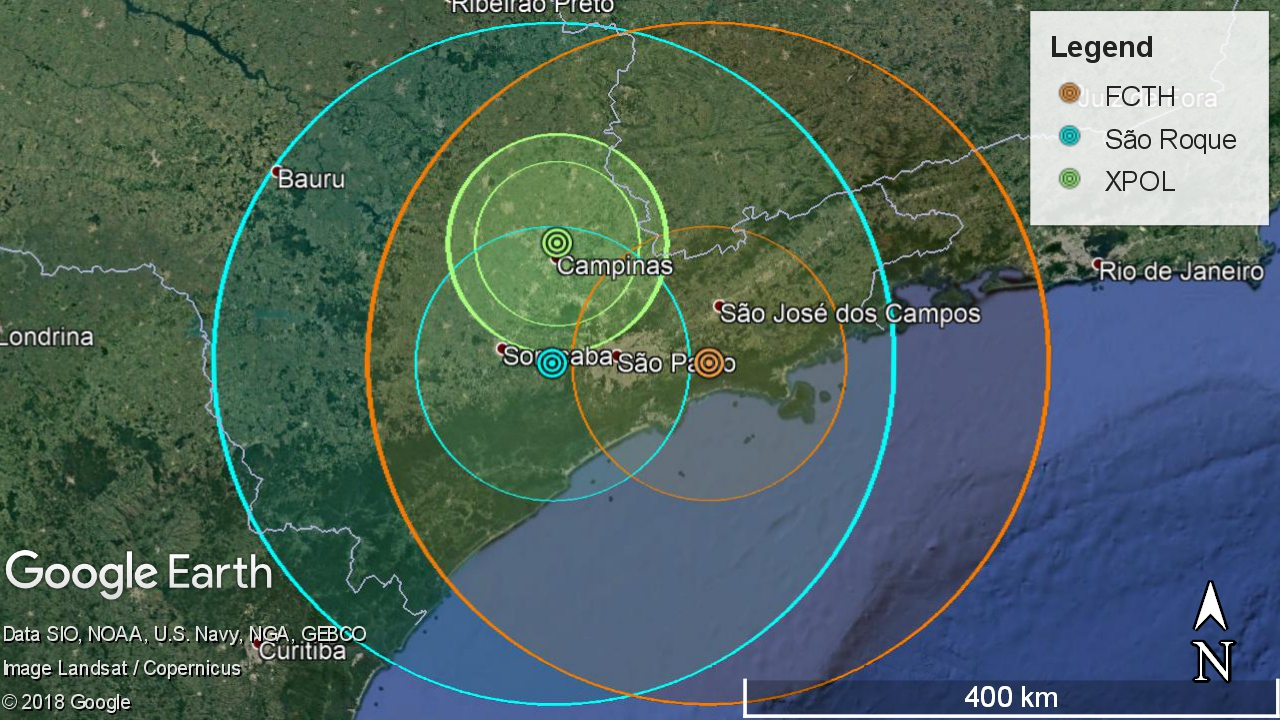
\includegraphics[width=\columnwidth]{figs/radar_coverages_hires2.jpg}
		\legend{Fonte: Produzido pela autora.}
	\end{center}
\end{figure}

O radar Doppler Banda-S de dupla polarização operado pela Fundação Centro Tecnológico de Hidráulica (FCTH) é localizado na barragem de Ponte Nova, município de Biritiba Mirim (\ang{23;36;}\:S, \ang{45;58;20}\:W, $916\:m$ de altitude). Este radar faz uma varredura volumétrica a cada 5 minutos em uma cobertura de até $250\:km$, com 8 elevações (\ang{1}, \ang{1,6}, \ang{2,4}, \ang{3,2}, \ang{4,2}, \ang{5,5}, \ang{6,9} e \ang{8,6}) de \ang{1} de abertura do feixe, como mostra a Figura\autoref{estrategia_cth}. A velocidade de Nyquist (valor máximo (mínimo no caso negativo) de velocidade radial medido) deste radar é de $16,27\:ms^{-1}$. Os dados volumétricos foram convertidos em uma grade de $1\:x\:1\:x\:1\:km$ usando o pacote Py-ART (\textit{Python ARM Radar Toolkit}, Conjunto de Ferramentas de Radar em Python do ARM) \cite{Helmus2016} e perfis horizontais (em $3\:km$ de altura) e verticais (cortes entre dois pontos com coordenadas latitudinais e longitudinais) foram analisados. Além da variável refletividade do radar (medida em $dBZ$), três variáveis polarimétricas foram analisadas e relacionadas com diferentes tipos de hidrometeoros seguindo a classificação de \citeonline{Straka2000} descrita na \autoref{hid}:

\begin{alineas}
	\item \textbf{Refletividade Diferencial ($dBZ$)}: Razão entre os fatores de refletividade horizontal e verticalmente polarizados; diferencia a forma das partículas em um dado volume medido;
	\item \textbf{Fase Diferencial Específica ($^\circ\:km^{-1}$)}: Calculada a partir das matrizes de espalhamento vertical e horizontal, é fortemente influenciada pela concentração numérica e massa de gotículas de nuvem, permitindo a derivação da distribuição de tamanho das mesmas;
	\item \textbf{Coeficiente de Correlação (adimensional)}: Razão entre as amplitudes das matrizes de espalhamento; destaca misturas de formas e tamanhos das partículas \cite{Rauber2018}.
\end{alineas}

O radar Doppler Banda-S operado pelo DECEA (Departamento de Controle do Espaço Aéreo) instalado em São Roque (\ang{23;35;56}\:S, \ang{47;5;52}\:W, $1147,54\:m$ de altitude) faz varreduras a cada 10 minutos em uma cobertura de até $250\:km$, com 15 elevações (\ang{0,5}, \ang{1}, \ang{2}, \ang{3}, \ang{4}, \ang{5}, \ang{6}, \ang{7}, \ang{8}, \ang{9}, \ang{10}, \ang{12}, \ang{14}, \ang{16} e \ang{18}) de \ang{2} de abertura do feixe, como mostra a Figura\autoref{estrategia_sr}. A velocidade de Nyquist deste radar é de $14,63\:ms^{-1}$. Os perfis horizontais de CAPPIs (\textit{Constant Altitude Plan Position Indicator}, Indicador Plano de Posição em Altitude Constante) em $3\:km$ de altura serviram como dados de entrada para o algoritmo ForTraCC (\textit{Forecast and Tracking the Evolution of Cloud Clusters}, Prevendo e Rastreando a Evolução de Aglomerados de Nuvens) \cite{Vila2008} adaptado para radares meteorológicos. Este algoritmo identifica os sistemas convectivos usando um limiar de refletividade - $35\:dBZ$ neste trabalho - e os classifica usando imagens subsequentes: sistema novo (\textit{new}), em continuidade (\textit{continuity}), em fusão (\textit{merge}) ou em separação (\textit{split}) - A \autoref{fortracc_teoria} mostra uma ilustração dessas situações.

\begin{figure}[htb]
	\begin{center}
		\caption{Representação dos tipos de classificação do ForTraCC: continuidade (a), separação (b) e fusão (c). As formas com contorno pontilhado representa o sistema no primeiro passo enquanto que as formas cinzas representam o sistema no passo seguinte, com as setas indicando o deslocamento} 
		\label{fortracc_teoria}
		%		\setcaptionmargin{1cm}
		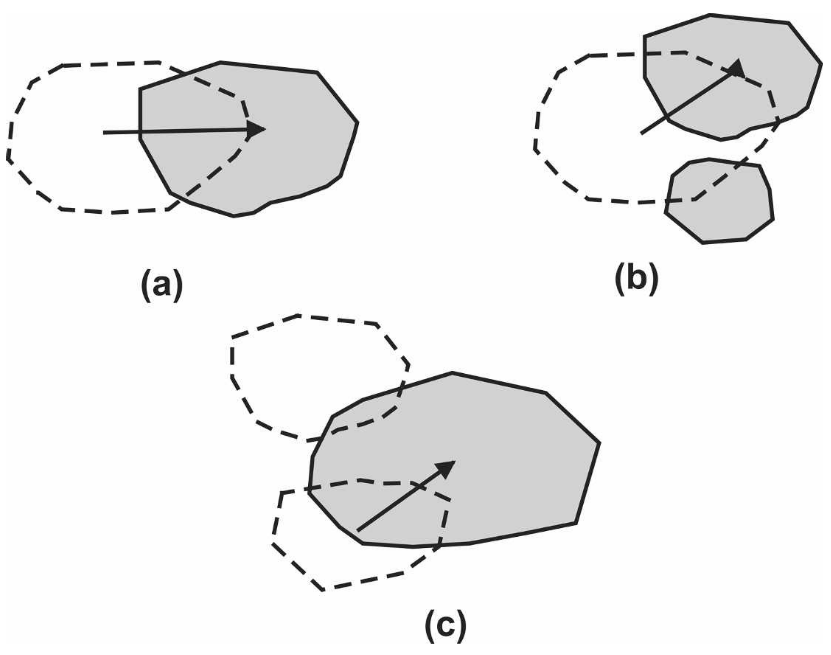
\includegraphics[width=0.5\columnwidth]{figs/fortracc_classes.png}
		\legend{Fonte: \citeonline{Vila2008}.}
	\end{center}
\end{figure}

O ciclo de vida da tempestade associada a cada caso foi definido a partir do sistema convectivo com maior intensidade na posição do hailpad, considerando o horário aproximado da queda de granizo. A partir desse sistema, a família - definição do algoritmo para um conjunto de sistemas próximos uns aos outros com mesmo deslocamento - associada a ele foi extraída e corrigida caso houvesse necessidade. A partir de cada rastreamento, variáveis como refletividade máxima e tamanho do sistema foram analisadas, além de servirem como base para a seleção de descargas elétricas associadas aos sistemas.

O radar Doppler Banda-X de dupla polarização XPOL foi operado pelo Projeto SOS-CHUVA na UNICAMP, cidade de Campinas (\ang{22;48;50}\:S, \ang{47;3;22}\:W, $680\:m$ de altitude). Ele fez varreduras volumétricas a cada 10 minutos em uma cobertura de até $80\:km$, com 17 elevações (\ang{0,5}, \ang{1,8}, \ang{3,1}, \ang{4,4}, \ang{5,7}, \ang{7}, \ang{8,3}, \ang{9,6}, \ang{10,9}, \ang{13}, \ang{15}, \ang{18}, \ang{22}, \ang{26}, \ang{32}, \ang{40} e \ang{55}) de \ang{1,3} de abertura do feixe, como mostra a Figura\autoref{estrategia_xpol}. Por ser de uma banda de frequência mais alta, a velocidade de Nyquist deste radar é menor do que a dos radares Banda-S: $9,6\:ms^{-1}$. Os dados volumétricos também foram convertidos em uma grade de $1\:x\:1\:x\:1\:km$ e as variáveis refletividade do radar e velocidade radial foram utilizadas. Devido à falta de dados em muitos dos casos selecionados, este radar foi usado apenas como entrada no algoritmo de recuperação de vento por Multi-Doppler (\autoref{multidoppler}) juntamente com os demais radares.

\begin{figure}[hp]
	\begin{center}
		\caption{Estratégia de varredura volumétrica dos radares meteorológicos da FCTH (a), de São Roque (b) e o XPOL instalado na UNICAMP (c)} 
		\label{estrategia_radares}
		\subfloat[]{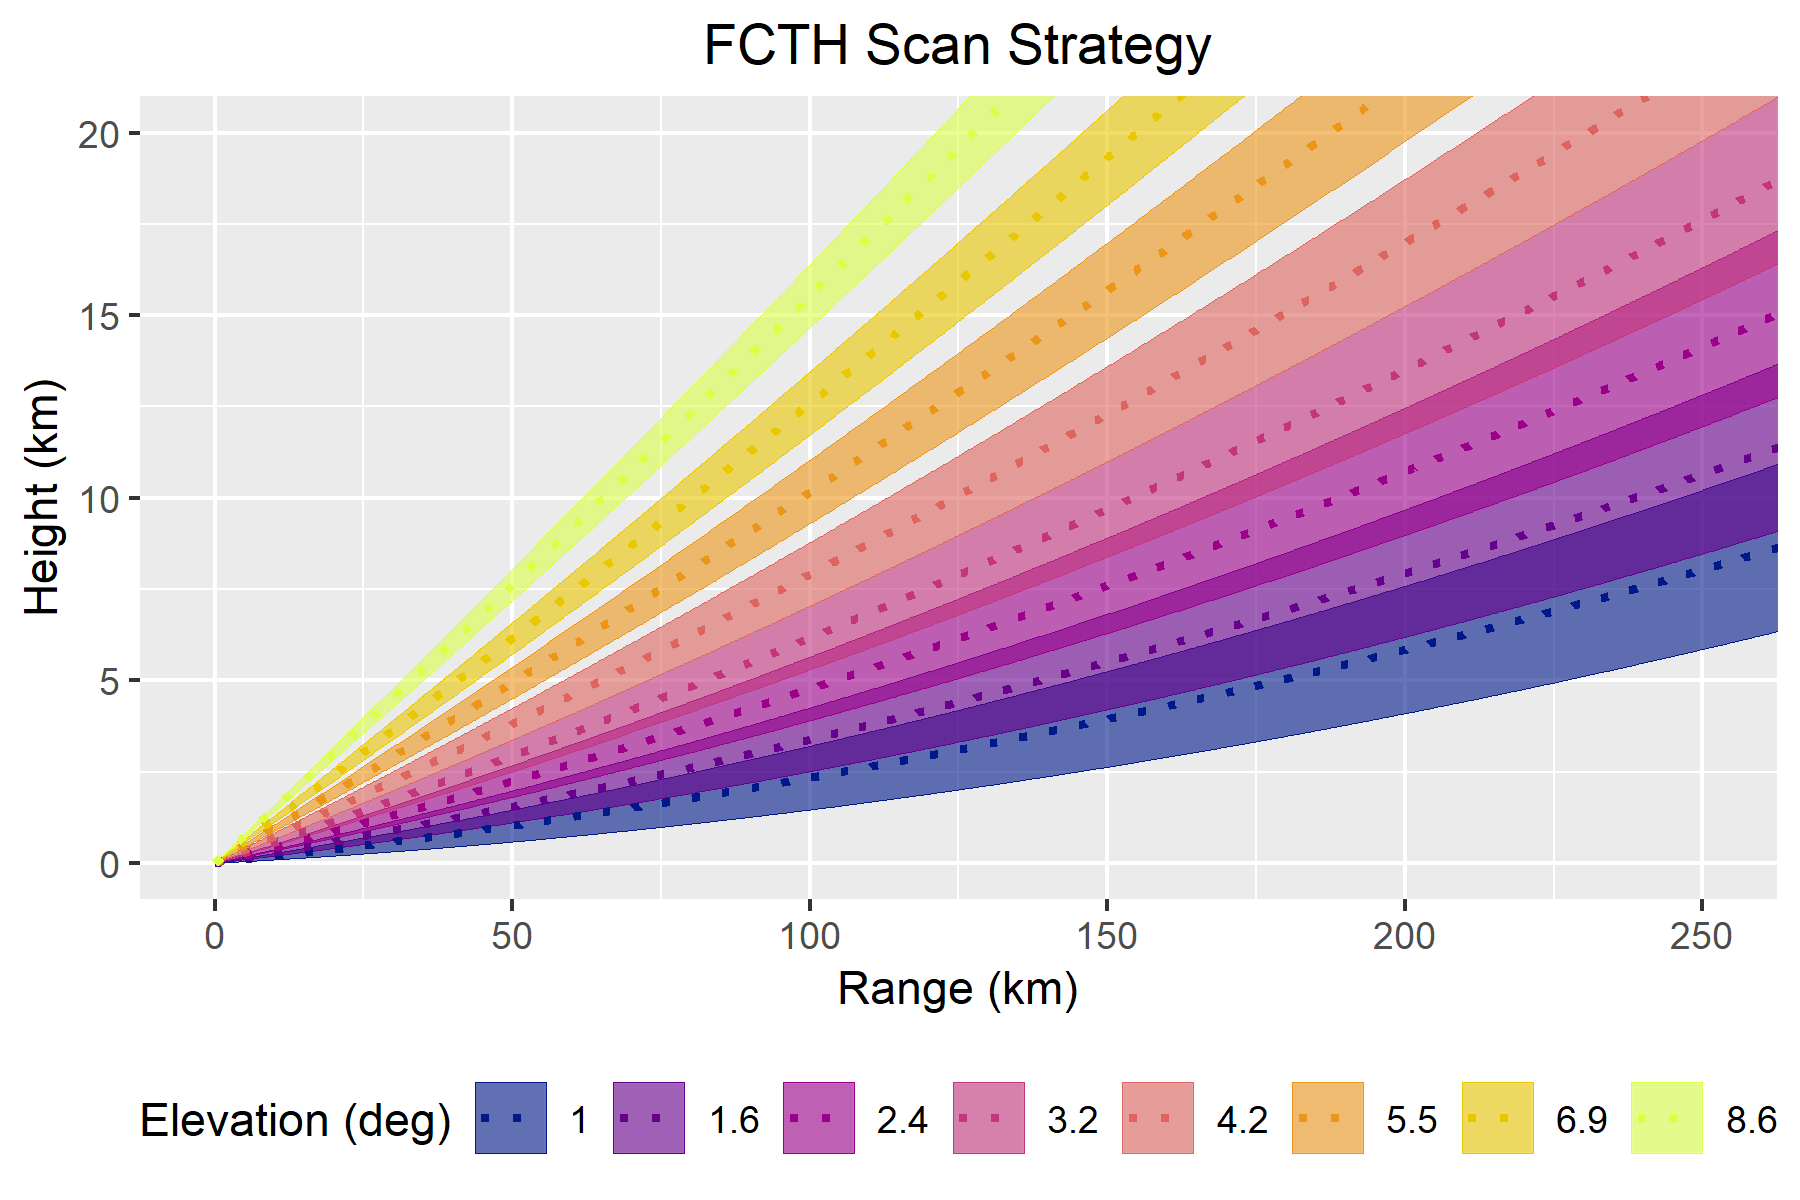
\includegraphics[width=0.75\columnwidth]{../General_Processing/figures/scan_strategy_cth.png}\label{estrategia_cth}}\\
		\subfloat[]{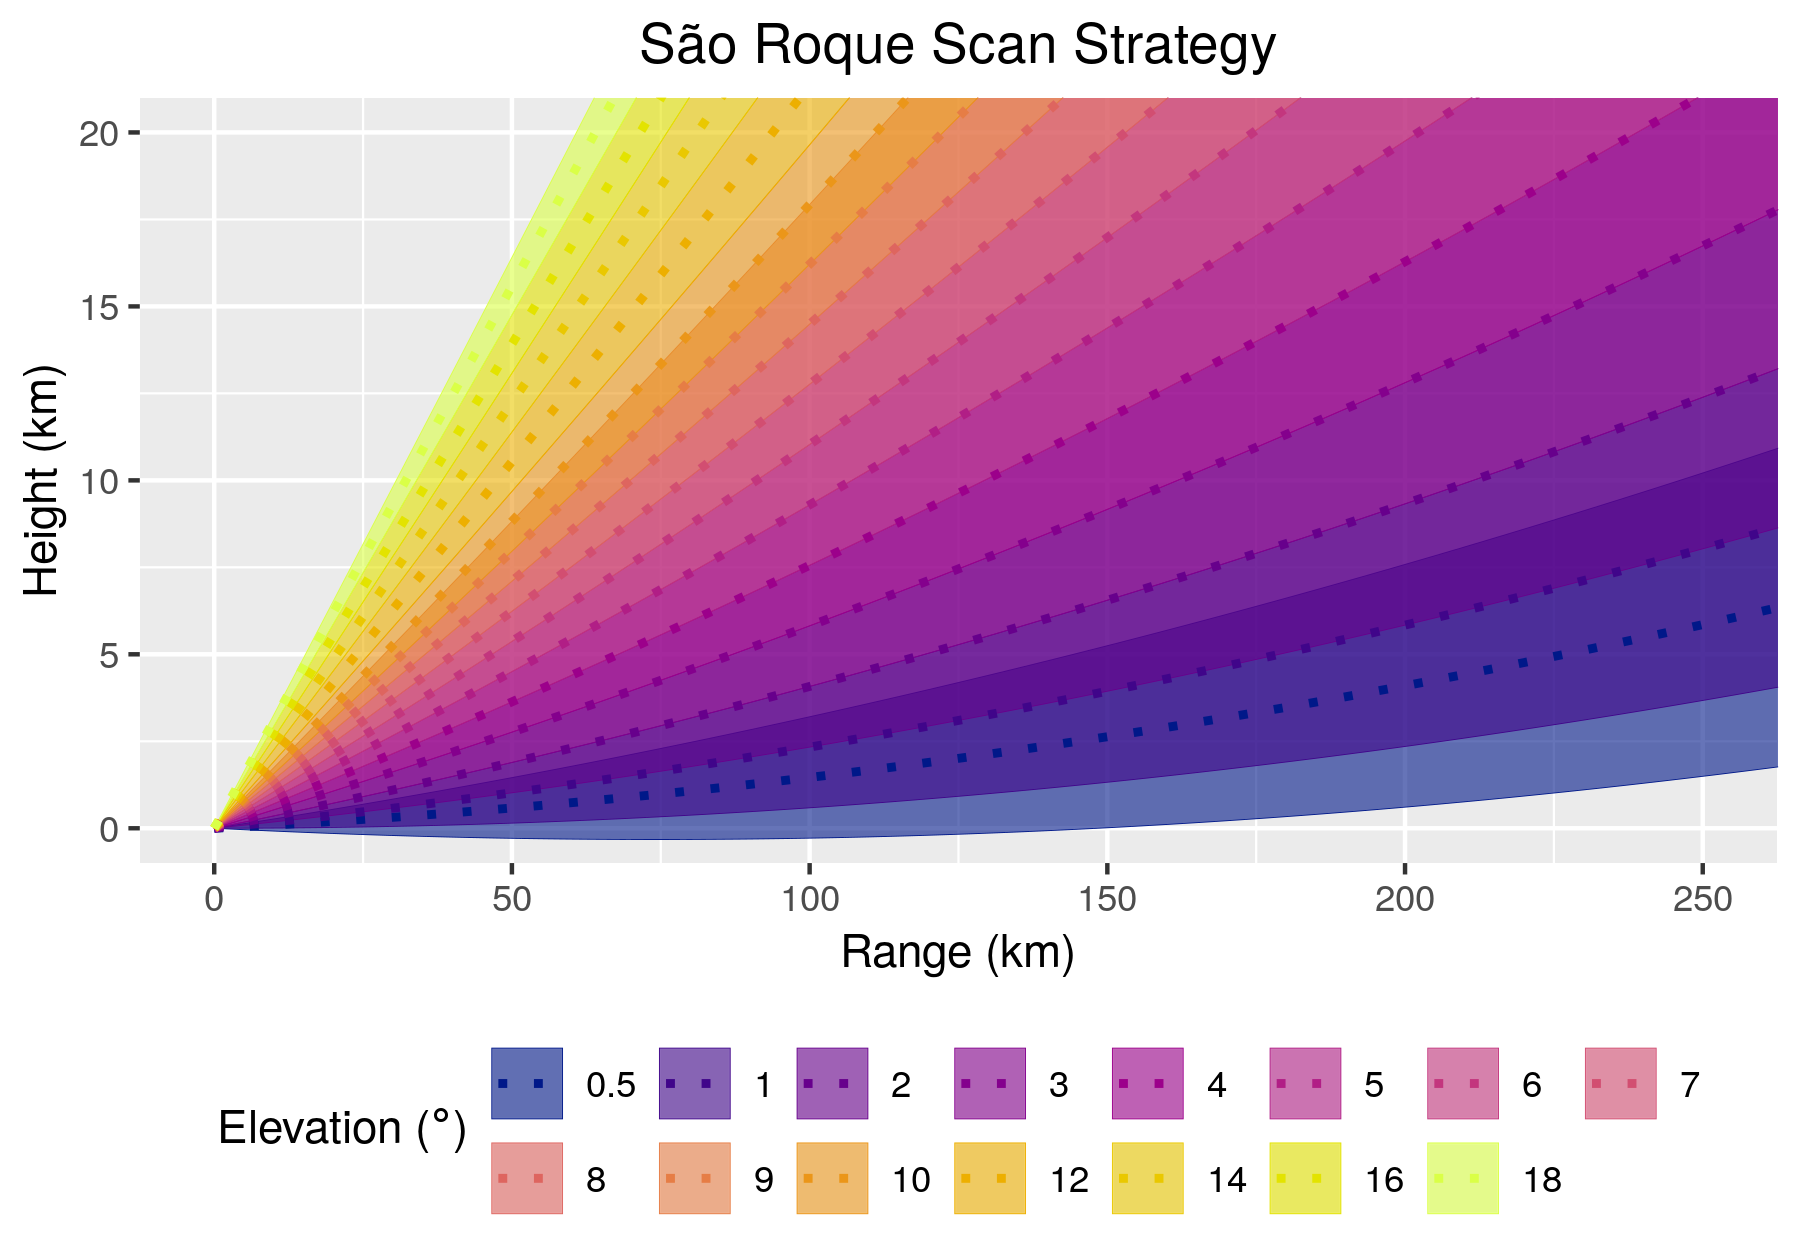
\includegraphics[width=0.75\columnwidth]{../General_Processing/figures/scan_strategy_sr.png}\label{estrategia_sr}}\\
		\subfloat[]{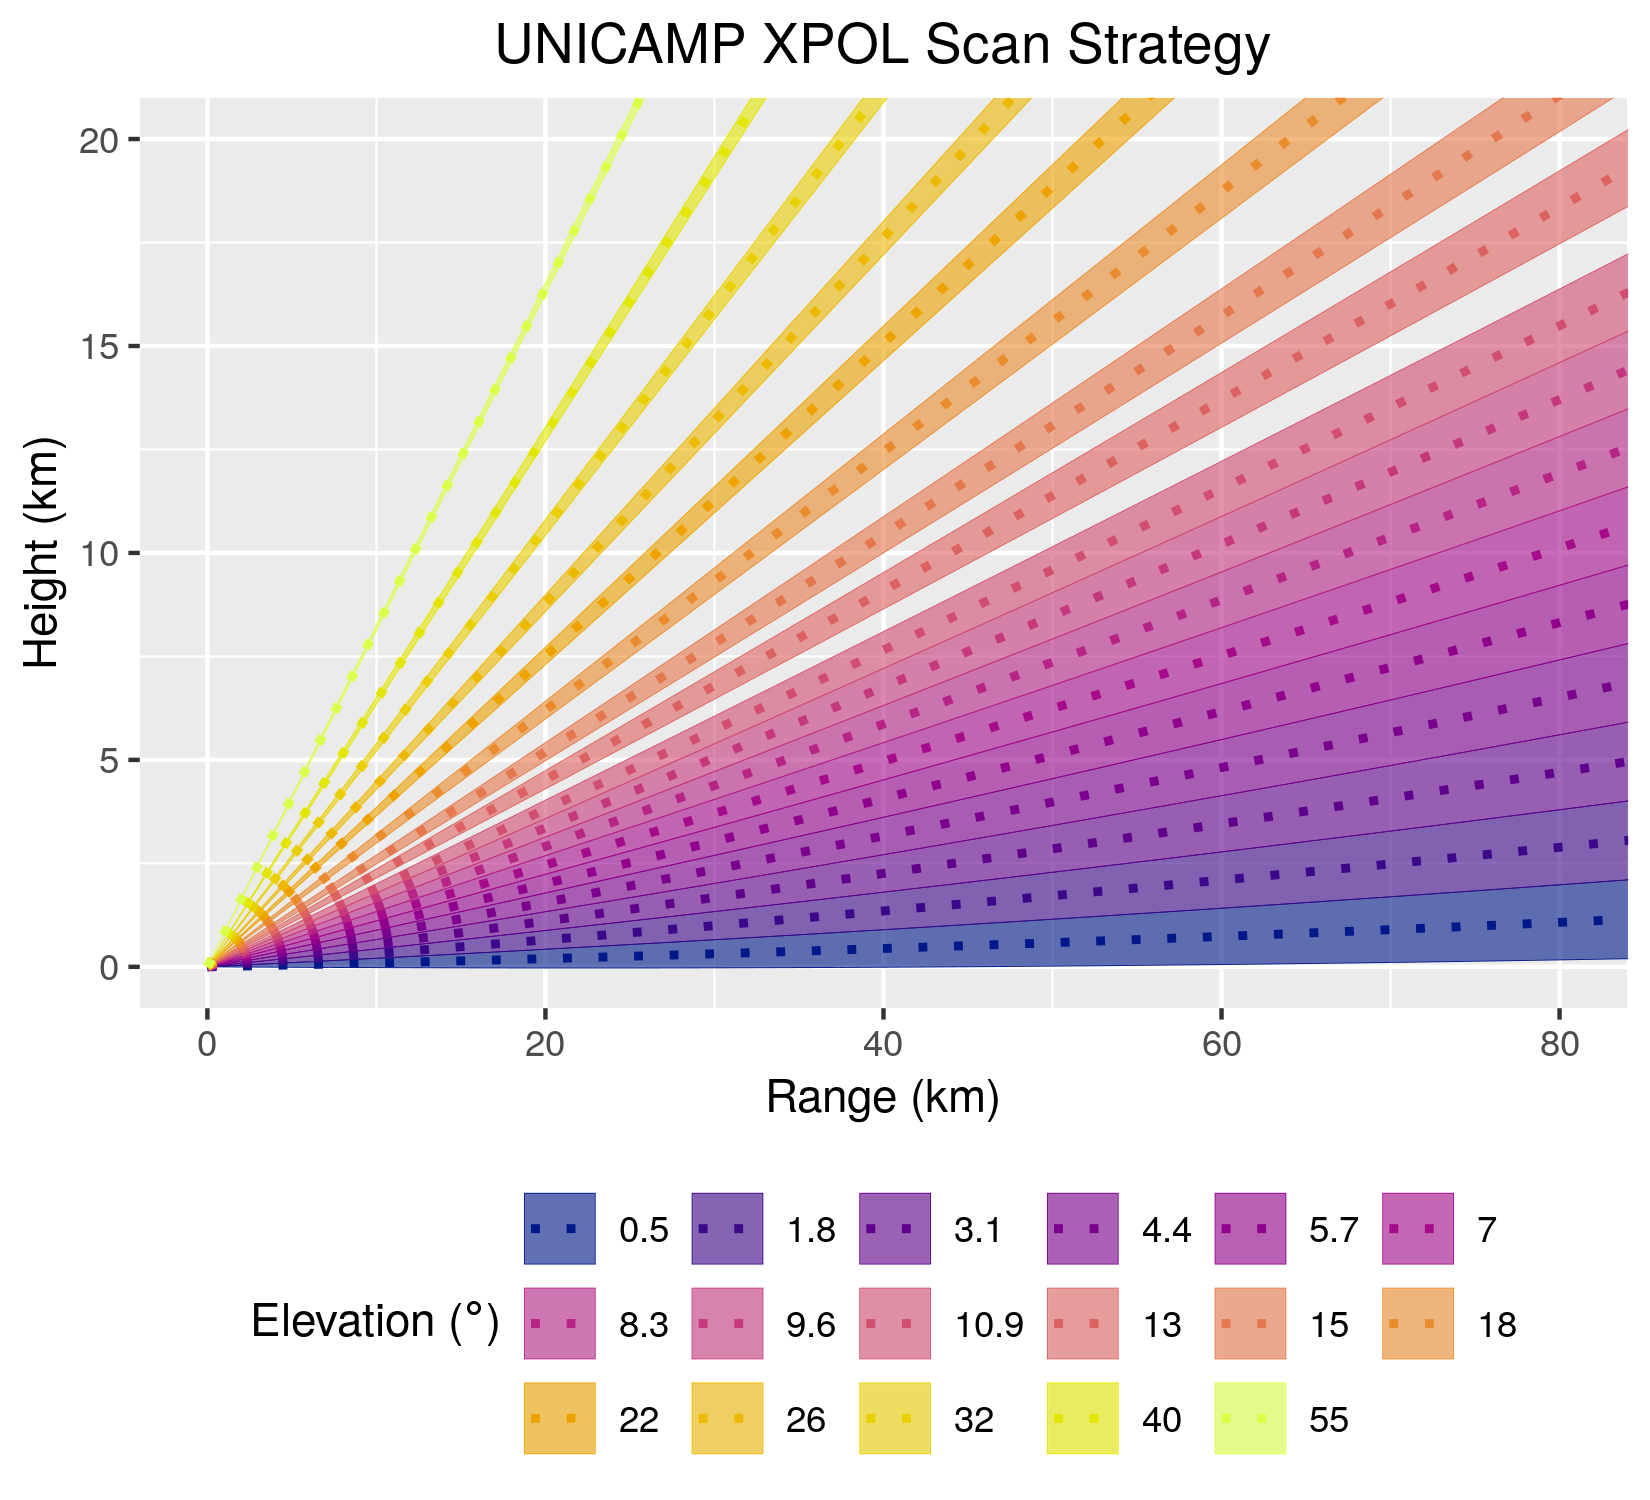
\includegraphics[width=0.75\columnwidth]{../General_Processing/figures/scan_strategy_xpol.png}\label{estrategia_xpol}}\\
		\legend{Fonte: Produzido pela autora.}
	\end{center}
\end{figure}

\subsection{Identificação de Hidrometeoros}\label{hid}

Para definir de forma mais acurada a presença de granizo nas medidas de radar, o método de classificação de hidrometeoros usando Lógica Fuzzy foi aplicado. Presente no pacote CSU\_RadarTools \cite{Lang2017a} através de uma função chamada \textit{Fuzzy Hydrometeor Classificator} (Classificador Fuzzy de Hidrometeoros), o método implementado é dividido em três passos:

\begin{alineas}
	\item A \textbf{fuzzificação} usa funções beta, que indicam a probabilidade de um dado valor de variável polarimétrica representar um dado tipo de hidrometeoro, com pesos específicos para cada variável (refletividade e temperatura apresentam o maior peso) para classificar os dados polarimétricos de entrada em cada ponto de grade;
	\item A \textbf{inferência} calcula uma pontuação para cada tipo de hidrometeoro somando as classificações de cada variável e;
	\item A \textbf{agregação} escolhe a pontuação máxima para cada ponto e indica o hidrometeoro correspondente a ela \cite{Liu2000a}.
\end{alineas}

Esta função é aplicada em tempestades de verão e diferencia 10 tipos de hidrometeoros:

\begin{alineas}
	\item Chuvisco (\textit{Drizzle})
	\item Chuva (\textit{Rain})
	\item Cristais de Gelo (\textit{Ice Crystals})
	\item Agregados (\textit{Aggregates})
	\item Neve Molhada (\textit{Wet Snow})
	\item Gelo Vertical (\textit{Vertical Ice})
	\item Graupel de Densidade Baixa (\textit{Low-Density Graupel})
	\item Graupel de Densidade Alta (\textit{High-Density Graupel})
	\item Granizo (\textit{Hail})
	\item Gotas Grandes (\textit{Big Drops})
\end{alineas}

A função utiliza como entrada os campos de refletividade, refletividade diferencial, fase diferencial específica e coeficiente de correlação, além de um perfil de temperatura obtido a partir de uma radiossondagem. As radiossondagens aplicadas foram coletadas no Campo de Marte (Estação SBMT, São Paulo) em datas próximas aos eventos e os dados foram processados usando o pacote Siphon \cite{siphon}.

Para verificar subjetivamente a performance do método de classificação de hidrometeoros, os campos de variáveis polarimétricas foram analisados e relacionados com os mesmos tipos de hidrometeoros do método a partir da classificação de \citeonline{Straka2000}. A \autoref{hid_straka} mostra os intervalos de valores de cada variável correspondente a cada tipo de hidrometeoro, incluindo também a mistura de chuva com granizo (\textit{rain + hail}).

\begin{figure}[htb]
	\begin{center}
		\caption{Classificação de hidrometeoros de acordo com refletividade (a), refletividade diferencial (b), fase diferencial específica (c) e coeficiente de correlação (ou razão de correlação cruzada) (d)} 
		\label{hid_straka}
%		\setcaptionmargin{1cm}
		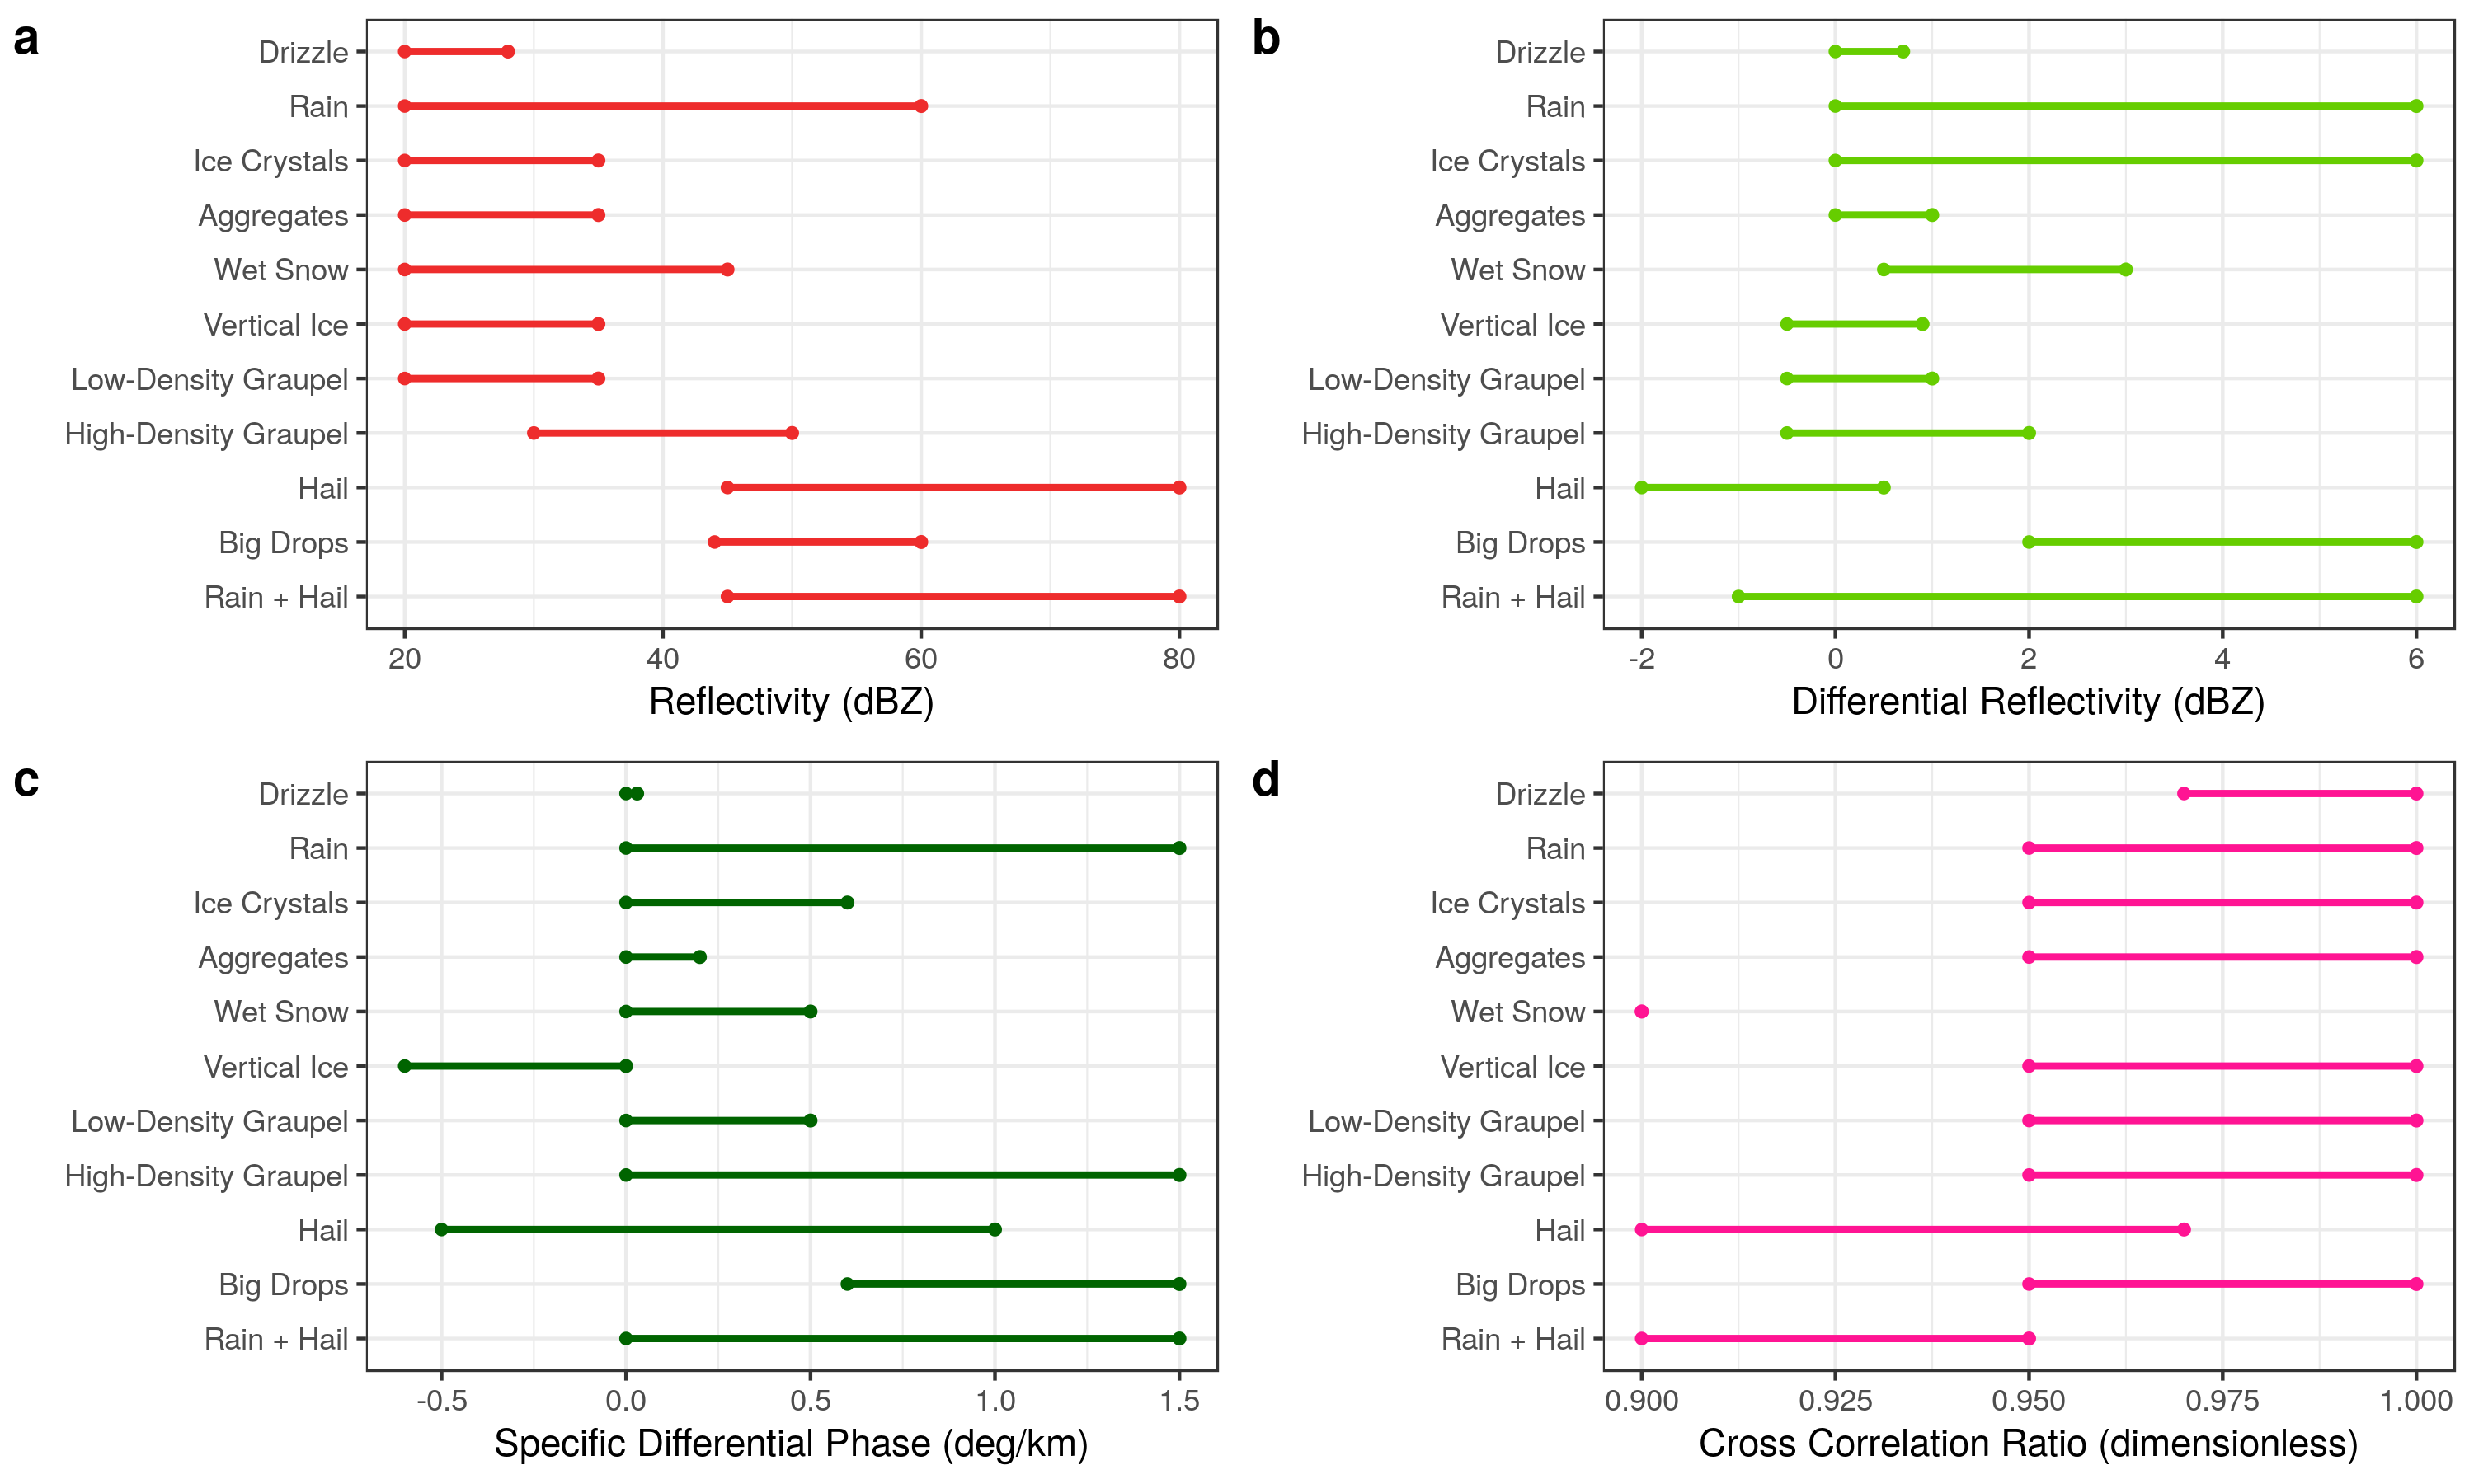
\includegraphics[width=\columnwidth]{../General_Processing/figures/hids_strakaetal.png}
		\legend{Fonte: Produzido pela autora a partir de \citeonline{Straka2000}.}
	\end{center}
\end{figure}

Outra função do pacote CSU\_RadarTools usada neste trabalho chama-se \textit{Liquid/Ice Water Mass Calculations} (Cálculos de Massas de Água Líquida e Gelo), que utiliza de entrada a refletividade e a refletividade diferencial. A partir do cálculo da contribuição da chuva para a refletividade horizontal - e consequentemente da contribuição do gelo através do resíduo da mesma - a massa de água líquida é derivada, usando a refletividade diferencial quando a água líquida é predominante. A massa de gelo é calculada apenas a partir da contribuição do gelo por uma aproximação de Rayleigh \cite{Carey2000, Cifelli2002b}.

\subsection{Recuperação de Vento por Multi-Doppler}\label{multidoppler}

A área de estudo possui cobertura de pelo menos dois radares - três se considerar a cobertura máxima dos radares (\autoref{cobertura_radares}) - capazes de medir velocidade radial (Doppler) quase simultaneamente (\autoref{tabela_radares_md}). Isso permite a aplicação de métodos que convertem os campos tridimensionais de refletividade e velocidade radial de múltiplas perspectivas em um campo tridimensional de velocidade do vento com alto grau de detalhamento.

\begin{table}[htb]
	\IBGEtab{%
		\caption{Configuração dos radares nos casos em que a recuperação de vento por Multi-Doppler foi utilizada}%
		\label{tabela_radares_md}
	}{%
		\begin{tabularx}{0.8\textwidth}{Yccccc}
			\toprule
			Caso & \multicolumn{2}{c}{2017-03-14} & \multicolumn{3}{c}{2017-11-15} \\
			\midrule 
			Radares disponíveis & FCTH & SR & FCTH & SR & XPOL \\
			\midrule 
			Resolução temporal ($s$) & $300$ & $600$ & $300$ & $600$ & $600$ \\ 
			\midrule 
			Diferença mínima entre os horários de começo da varredura dos radares ($s$) & \multicolumn{2}{c}{$172$} & \multicolumn{3}{c}{$19$} \\
			\midrule
			Diferença máxima entre os horários de começo da varredura dos radares ($s$) & \multicolumn{2}{c}{$174$} & \multicolumn{3}{c}{$20$} \\
			\bottomrule
		\end{tabularx}%
	}{%
		\fonte{Produzido pela autora.}%
	}
\end{table}

A base teórica do método de recuperação de vento tridimensional foi estabelecida por \citeonline{Armijo1969}. Ela consiste em determinar 4 componentes da velocidade do vento em coordenadas cartesianas: $u$, $v$, $w$ e $w_t$, onde as três primeiras são as componentes da velocidade nas coordenadas $x$, $y$ e $z$ e $w_t$ é a velocidade terminal da precipitação \cite{Rinehart1997}. Dois radares Doppler vendo a mesma tempestade de ângulos diferentes fornecem duas medidas distintas de velocidade radial ($v_{r_1}$ e $v_{r_2}$), como mostra a \autoref{doviak_sistema}, e $w_t$ pode ser estimada em função da refletividade (usando uma distribuição de Marshall-Palmer, por exemplo). Assim, $u$ e $v$ podem ser descritos como:

\begin{figure}[htb]
	\begin{center}
		\caption{Sistema de coordenadas cilíndricas usado para análise Dual-Doppler de dados de radar. Os radares estão localizados nos pontos 1 e 2 e $a_r$, $a_s$ e $a_\alpha$ são as normais unitárias definindo a direção das três componentes ortogonais da velocidade. O eixo cilíndrico está ao longo da linha conectando os radares (separados por uma distância $2d$) e $r$ é a distância do eixo ao dado pontual} 
		\label{doviak_sistema}
		%		\setcaptionmargin{1cm}
		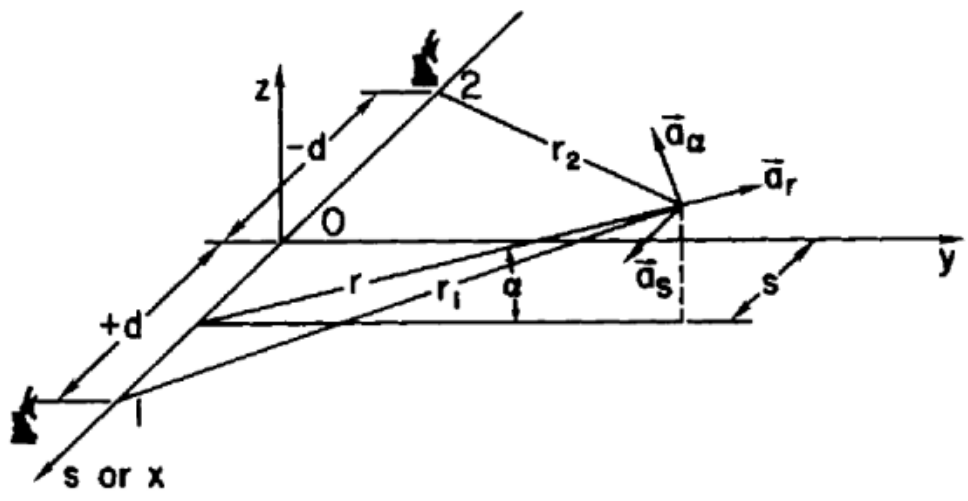
\includegraphics[width=0.8\columnwidth]{figs/system_doviak.png}
		\legend{Fonte: \citeonline{Doviak1993}}
	\end{center}
\end{figure}

\begin{equation}
	u=\frac{1}{\sin{(\theta_1 - \theta_2)}}\left(\frac{v_{r_1}\cos{\theta_2}}{\sin{\alpha_1}}-\frac{v_{r_2}\cos{\theta_2}}{\sin{\alpha_2}}\right)
\end{equation}

\begin{equation}
	v=\frac{1}{\sin{(\theta_1 - \theta_2)}}\left(\frac{v_{r_2}\cos{\theta_1}}{\sin{\alpha_2}}-\frac{v_{r_1}\cos{\theta_1}}{\sin{\alpha_1}}\right)
\end{equation}

\noindent
onde $\theta_1$ e $\theta_2$ são os ângulos azimutais dos radares $1$ e $2$, respectivamente, e $\alpha_1$ e $\alpha_2$ são os ângulos de elevação dos mesmos.

Para calcular a componente vertical da velocidade, a equação de continuidade de massa é usada, assumindo como condições de contorno que a velocidade na superfície e no topo da tempestade são nulas, ou seja:

\begin{equation} 
	\label{continuidade_massa}
	\frac{\partial(\rho w)}{\partial z}=-\rho\left(\frac{\partial u}{\partial x} + \frac{\partial v}{\partial y}\right)
\end{equation}

\begin{equation}
	w=w_T-w_t
\end{equation}

\noindent
onde $\rho$ é a densidade do ar atmosférico e $w_T$ é a velocidade vertical total. Quando três radares são usados, é possível calcular o campo tridimensional sem usar a \autoref{continuidade_massa}.

Ao combinar radares Doppler para a recuperação do vento, a área de cobertura e erros característicos (altura do feixe e resolução espacial) devem ser considerados \cite{Dolan2007}. Se a distância da linha de base entre os dois radares for longa, a área de cobertura será maior mas a resolução espacial será prejudicada. Além disso, se o ângulo de cruzamento do feixe é pequeno (mais paralelo), as duas medidas serão mais similares e as variâncias dos erros de velocidade nas estimativas Dual-Doppler - $\sigma_u^2$ e $\sigma_v^2$ - serão menores. De acordo com \citeonline{Davies-Jones1979}, $\sigma_u^2$ e $\sigma_v^2$ estão relacionadas com as variâncias dos erros de velocidade Doppler de cada radar, $\sigma_1^2$ e $\sigma_2^2$, da seguinte forma:

\begin{equation}
	\frac{\sigma_u^2+ \sigma_v^2}{\sigma_1^2 + \sigma_2^2}=\csc^2{\beta}
\end{equation}

\noindent
onde $\beta$ é o ângulo de cruzamento do feixe entre os dois radares. Para $\beta\:<\:\ang{30}$, $\sigma_u^2$ e $\sigma_v^2$ crescem rapidamente \cite{Doviak1976, Davies-Jones1979, Doviak1993}.

A \autoref{doppler_theory_lobes} mostra teoricamente as áreas aceitáveis para estimativa de velocidade do vento considerando dois valores de $\beta$: $\ang{30}$ e $\ang{45}$. Quanto maior o valor de $\beta$, melhor é a estimativa Dual-Doppler, mas menor será a área de cobertura dessa estimativa.

\begin{figure}[htb]
	\begin{center}
		\caption{Ângulos teóricos de cruzamento do feixe com Dual-Doppler de \ang{45} (melhores dados de vento) e \ang{30} (dados de vento aceitáveis) para um par de radares Doppler} 
		\label{doppler_theory_lobes}
		%		\setcaptionmargin{1cm}
		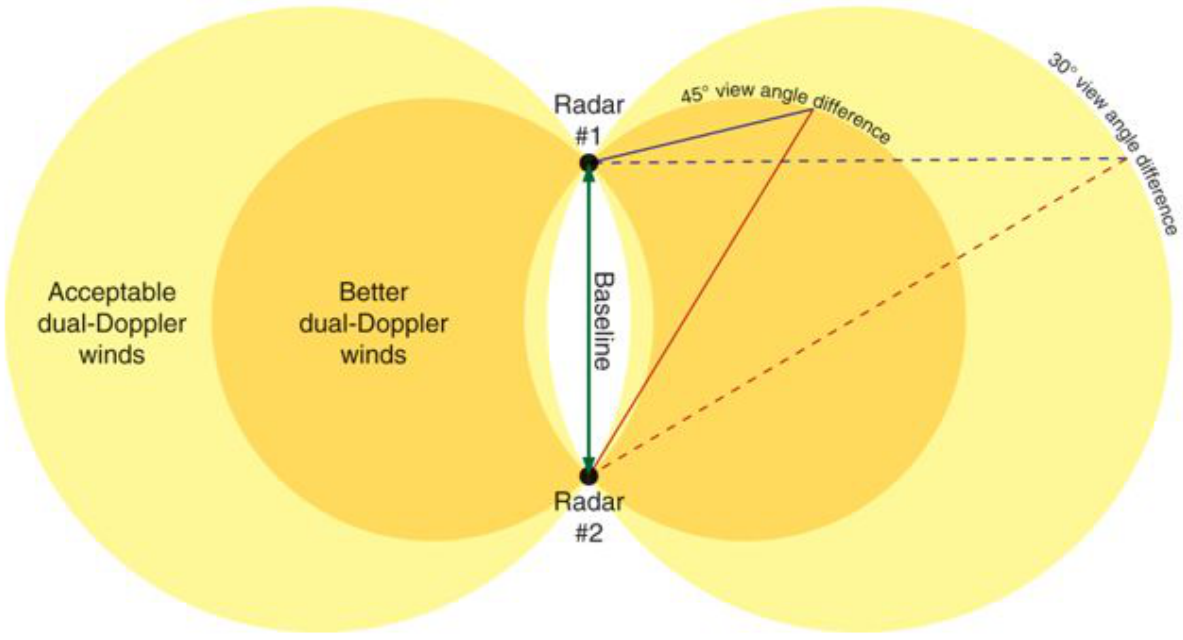
\includegraphics[width=\columnwidth]{figs/lobes_eastin.png}
		\legend{Fonte: Dr. Matthew D. Eastin, UNC.}
	\end{center}
\end{figure}

A \autoref{doppler_lobes} mostra o mesmo da \autoref{doppler_theory_lobes}, mas para combinações entre os três radares usados neste trabalho. Considerando a combinação FCTH/XPOL (painel superior), a distância entre os radares e a localização do XPOL dentro da cidade de Campinas limita as estimativas boas ou aceitáveis em boa parte da região de estudo, com exceção da cidade de Indaiatuba e à oeste dela. Considerando a combinação SR/FCTH (painel central), a estimativa Dual-Doppler tem erros menores (ou seja, $\beta=\ang{45}$) em Campinas e Indaiatuba (cidades com mais casos de queda de granizo, \autoref{tabela_casos}) e à leste, mas estimativas aceitáveis (ou seja, $\beta=\ang{30}$) estão disponíveis para toda a RMC. Considerando a combinação SR/XPOL (painel inferior), os ventos à nordeste e sudeste da RMC não podem ser estimados pois esses radares estão praticamente alinhados na direção norte-sul. A partir dessas considerações e da disponibilidade de dados para cada caso (\autoref{tabela_radares_md}), definiu-se que as combinações SR/FCTH e SR/FCTH/XPOL serão usadas para os casos 2017-03-14 e 2017-11-15, respectivamente.

\begin{figure}[hp]
	\begin{center}
		\caption{Ângulos de cruzamento do feixe com Dual-Doppler de \ang{45} (melhores dados de vento) e \ang{30} (dados de vento aceitáveis) para um par de radares Doppler, mais especificamente para as combinações dos radares FCTH e XPOL, São Roque (SR) e FCTH e SR e XPOL. Os contornos em cinza representam as cidades de São Paulo, Indaiatuba e Campinas, enquanto que as linhas pontilhadas indicam as distâncias entre os radares} 
		\label{doppler_lobes}
		%		\setcaptionmargin{1cm}
		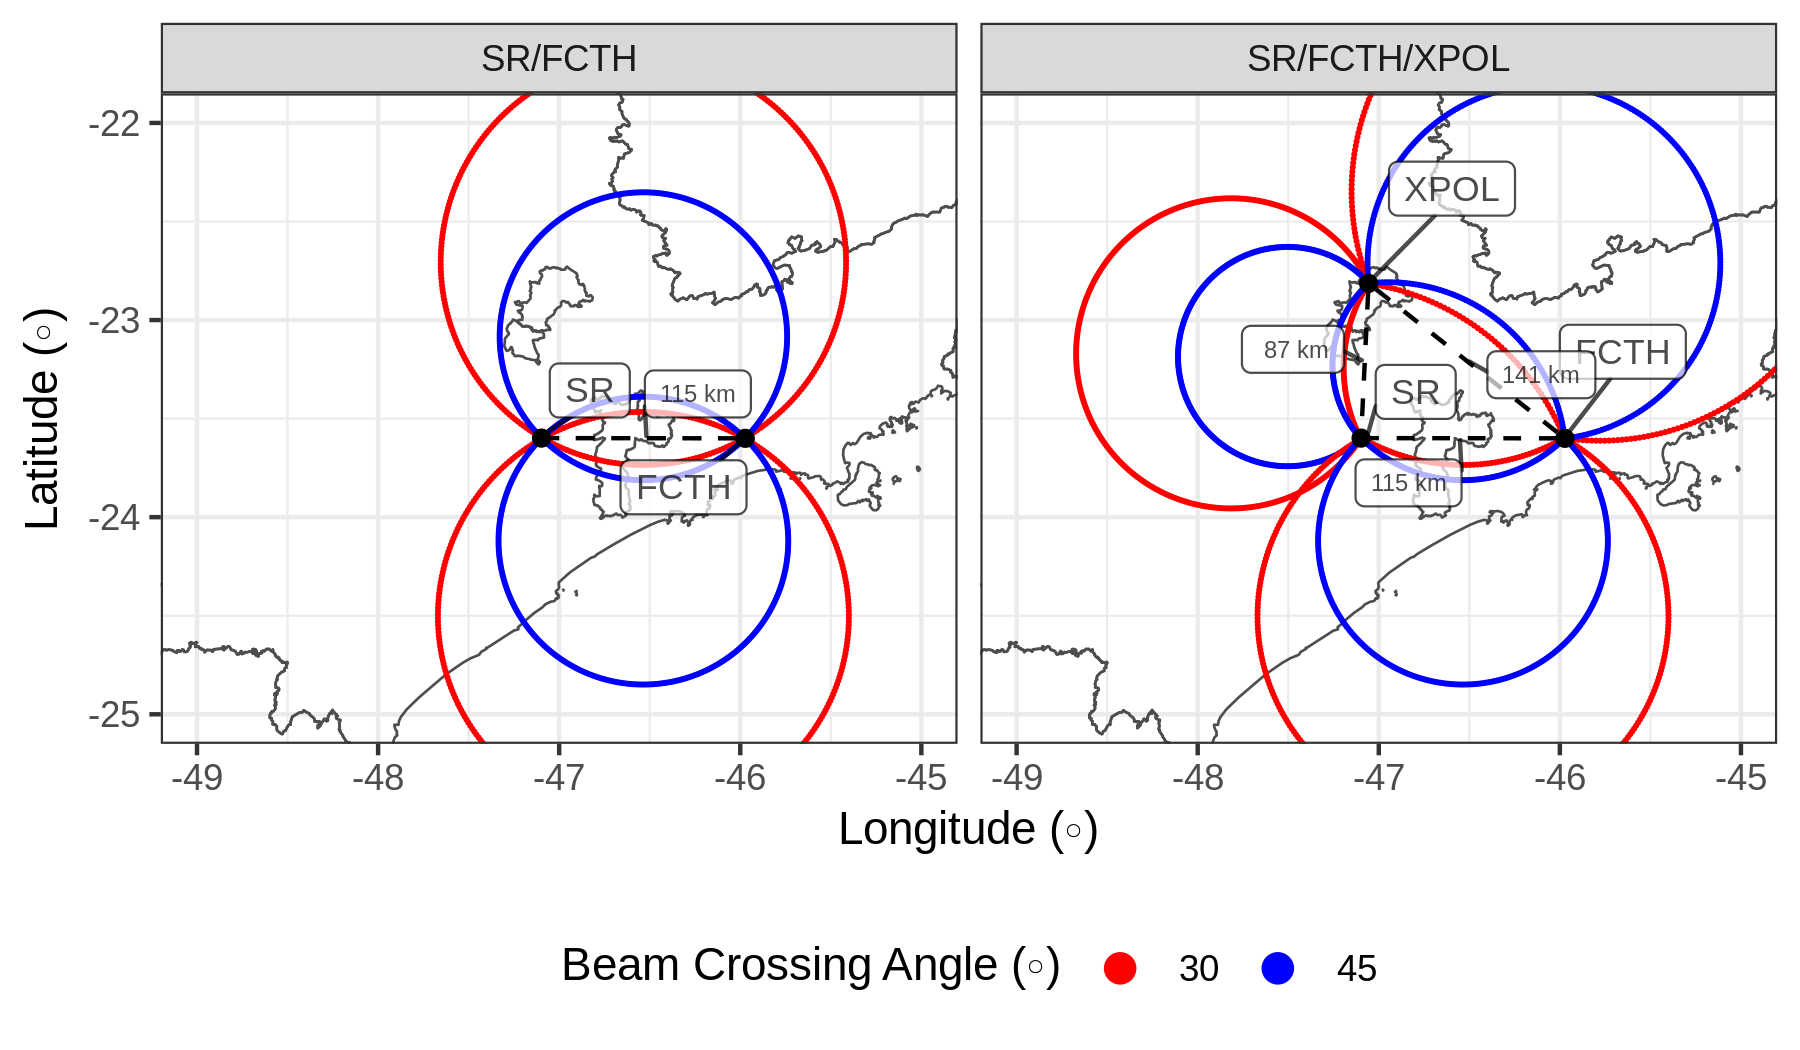
\includegraphics[width=0.65\columnwidth]{../General_Processing/figures/dual_doppler_lobes.png}
		\legend{Fonte: Produzido pela autora.}
	\end{center}
\end{figure}

Para calcular as estimativas de vento usando Dual e Multi-Doppler, o pacote MultiDop \url{https://github.com/nasa/MultiDop} foi utilizado. Desenvolvido em Python e C a partir da metodologia de \citeonline{Shapiro2009} e \citeonline{Potvin2012b} e compatível com o pacote Py-ART \cite{Helmus2016}, este pacote extrai o campo tridimensional de velocidade do vento a partir de uma combinação de 2 ou 3 radares. A metodologia usada nos cálculos é baseada em 3DVAR (\textit{3D Variational Analysis}, Análise Variacional em 3D), em que as componentes cartesianas do vento $u$, $v$ e $w$ são calculadas minimizando uma função custo total $J$ que quantifica erros nas restrições relacionadas aos dados ($J_O$), às equações de conservação de massa ($J_M$) e vorticidade ($J_V$) e à suavização ($J_S$):

\begin{equation}
	J=J_O+J_M+J_V+J_S
\end{equation}

Cada função custo é equivalente ao erro multiplicado por um coeficiente de ajuste $C$, que define o peso que esse erro terá no valor final de velocidade do vento \cite{Potvin2012b}. O pacote MultiDop permite que esses coeficientes sejam definidos pelo usuário - a \autoref{tabela_multidop} mostra os coeficientes escolhidos para as análises, similares a \citeonline{Potvin2012b}, além de outras configurações.

\begin{table}[htb]
	\IBGEtab{%
		\caption{Parâmetros de configuração do MultiDop para cálculos de Dual e Multi-Doppler.}%
		\label{tabela_multidop}
	}{%
		\begin{tabularx}{\textwidth}{YY}
			\toprule
			Resolução da grade & $1 \times 1 \times 1\:km$ \\
			\midrule
			Restrição da conservação de massa & Aproximação anelástica \\
			\midrule 
			Restrição de suavização & Derivadas de segunda ordem \\
			\midrule 
			Pesos na restrição de dados & Pesos iguais para todas as observações \\
			\midrule 
			Condição inicial da tempestade (deslocamento constante) & $U_t = V_t = -10\:ms^{-1}$ \\
			\midrule 
			Impor $w=0$ no topo & Sim \\
			\midrule
			Coeficiente da restrição dos dados & $1$ \\
			\midrule 
			Coeficiente da restrição da equação de continuidade de massa & $30$ \\
			\midrule 
			Coeficiente da restrição da equação de vorticidade & $1e^{-3}$ \\
			\midrule 
			Coeficiente de suavização horizontal & $1e^{-2}$ \\
			\midrule 
			Coeficiente de suavização vertical & $1e^{-2}$ \\
			\midrule
			Coeficiente da restrição da sondagem & $0$ \\
			\midrule 
			Todos os pesos constantes & Sim \\
			\midrule 
			Filtros & Nenhum \\
			\midrule 
			Estatísticas de verificação computadas apenas dentro do domínio de 2+ radares Doppler & Sim \\
			\midrule 
			Critério do domínio & 10 pontos \\
			\midrule
			Altura de corte & $0\:km$ \\
			\midrule 
			Matrizes de cobertura de fundo para ângulos de cruzamento de feixe ótimos para dois radares & Sim para todas as combinações \\
			\midrule 
			Matrizes de cobertura de fundo para ângulos de cruzamento de feixe aceitáveis para dois radares & Sim para todas as combinações \\
			\midrule 
			Matrizes de cobertura de fundo para um radar individual & Não para todos \\
			\midrule 
			Multiplicador do peso dos dados quando todos os radares tem bons ângulos de cruzamento do feixe & $SR=1e^{-3}$, $FCTH=XPOL=1$\\
			\bottomrule
		\end{tabularx}%
	}{%
		\fonte{Produzido pela autora.}%
	}
\end{table}


Como mostrado na \autoref{tabela_multidop}, os dados de radar foram convertidos para uma grade de $1\:x\:1\:x\:1\:km$. Além disso, problemas de ambiguidade da velocidade radial - quando a velocidade radial é maior do que a velocidade de Nyquist (\autoref{nyquist}) - foram corrigidos usando algoritmos baseado na região (analisa os dados por região de velocidades parecidas) e baseado em um esquema em quatro dimensões (4DD, \textit{Four-Dimensional Doppler Dealising Scheme}) \cite{James2001}, ambos presentes no pacote Py-ART; no caso do algoritmo 4DD, uma radiossondagem (novamente da estação do Campo de Marte) foi utilizada como condição inicial. Como forma de complementar as correções automáticas, correções manuais dos dados de velocidade radial foram feitas usando o software Solo3 \url{https://www.eol.ucar.edu/software/solo3}.

\begin{figure}[htb]
	\begin{center}
		\caption{Velocidade radial verdadeira vs medida de um alvo com uma velocidade de Nyquist de $10\:ms^{-1}$ mostrando a ambiguidade para valores de velocidade verdadeira além do intervalo de $-10$ a $10\:ms^{-1}$} 
		\label{nyquist}
		%		\setcaptionmargin{1cm}
		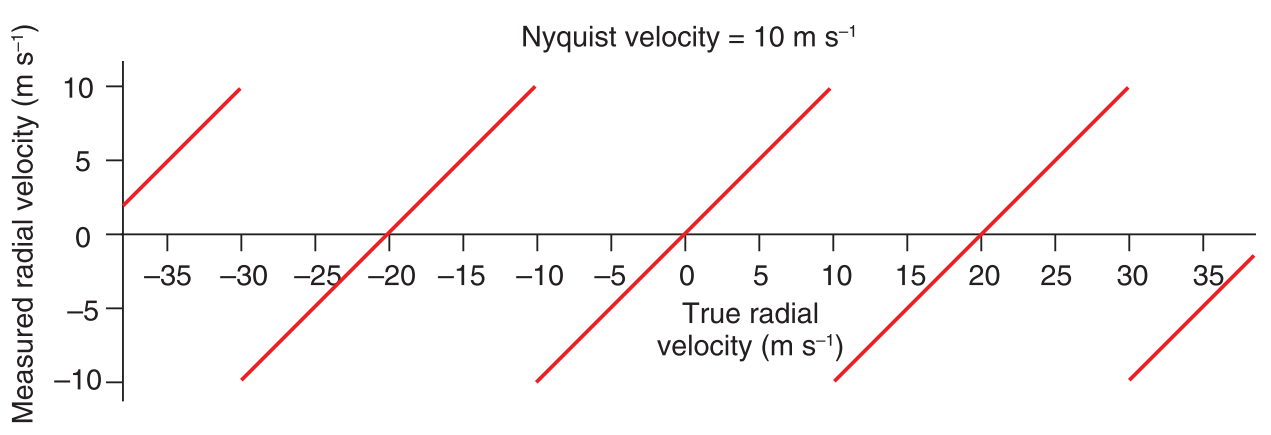
\includegraphics[width=\columnwidth]{figs/nyquist_rauber.png}
		\legend{Fonte: \citeonline{Rauber2018}.}
	\end{center}
\end{figure}

\section{Rede de Detecção de Raios}\label{raios}

A atividade elétrica dos casos selecionados foi analisada através dos dados do Sistema Brasileiro de Detecção de Descargas Elétricas (BrasilDAT) \cite{Naccarato2014}. Essa rede opera entre as faixas de frequência LF (\textit{Low Frequency}, Baixa Frequência) e HF (\textit{High Frequency}, Alta Frequência), detectando pulsos eletromagnéticos - chamados de strokes neste trabalho - emitidos pelas descargas elétricas através da técnica do tempo de chegada \cite{Lewis1960}. Devido à larga banda de frequência, é possível diferencial descargas de retorno de raios nuvem-solo (\textit{cloud-to-ground}, CG) e pulsos de raios intranuvem (\textit{intra-cloud}, IC), além de estimar a polaridade dos raios nuvem-solo através do sinal do pico de corrente. A eficiência de detecção estimada da rede é de $60$ a $70\%$ para raios IC e de $95\%$ para raios CG (Dr. Kleber Naccarato, ELAT-CCST-INPE, comunicação pessoal, 2018). Os dados dessa rede foram fornecidos pelo Grupo de Eletricidade Atmosférica (ELAT) do INPE e agrupados em flashes (\autoref{strokestoflashes}).

\subsection{Conversão Strokes-Flashes}\label{strokestoflashes}

Devido ao fato de que strokes estão associados a descargas de retorno e pulsos que não necessariamente representam raios distintos (um raio nuvem-solo, por exemplo, pode ser constituído de diversas descargas de retorno), esses dados foram convertidos em flashes, que representam todo o evento de uma descarga elétrica \cite{MacGorman1998b}. De acordo com \citeonline{Cummins1998} e \citeonline{Murphy2015}, strokes devem ser agrupados em flashes seguindo as seguintes considerações:

\begin{alineas}
	\item Strokes devem ser agrupados em um período total de $1\:s$, com intervalo entre strokes de até $500\:ms$;
	\item Strokes subsequentes devem estar em um raio de até $10\:km$ a partir do primeiro; pode-se considerar strokes subsequentes em um raio de até $50\:km$, desde que esteja dentro do intervalo de $500\:ms$;
	\item A multiplicidade de um flash (quantidade de strokes em um único flash) pode ser de até 63 (1023) strokes CG (IC).
\end{alineas} 

Para fazer o agrupamento seguindo as orientações acima, o algoritmo DBSCAN (\textit{Density-Based Spatial Clustering of Application with Noise}, Agrupamento Espacial Baseado em Densidade de Aplicação com Ruído) de agrupamento de dados foi utilizado. Ele usa a distância entre pontos $\epsilon$ e a quantidade mínima de pontos $min_{pts}$ para agrupar qualquer matriz de dados n-dimensional \cite{Ester1996, Kriegel2011}. \citeonline{Hutchins2014} e \citeonline{Hutchins2014a} usaram este método para agrupar strokes em flashes e em conjuntos de tempestades com raios, e a mesma abordagem foi adotada neste trabalho.

Como o algoritmo DBSCAN usa apenas dois parâmetros ($\epsilon$ e $min_{pts}$), enquanto que o agrupamento de strokes em flashes precisa de três (distância entre pontos $\epsilon_{spc}$, distância temporal $\epsilon_{t}$ e quantidade mínima de pontos $min_{pts}$), duas etapas são necessárias: agrupar os dados em função do tempo (usando $\epsilon_{t}$) e depois agrupar em função do espaço bidimensional (usando $\epsilon_{\text{spc}}$ em latitude e longitude). A partir das orientações de \citeonline{Cummins1998} e \citeonline{Murphy2015} e após alguns testes com $\epsilon_{spc}$ (\refanexo{anexo_conversao}), definiu-se que $min_{pts}=1$, $\epsilon_{t}=0,5\:s$ e $\epsilon_{spc}=2,5\:km$. O algoritmo foi implementado e adaptado usando a linguagem R.

A \autoref{flash_stats} mostra as características dos dados de flashes gerados usando as especificações acima. É possível observar que a distribuição de tempos entre strokes e entre flashes (\autoref{flash_stats}a) apresentam picos em aproximadamente $0,1$ e $1\:s$, respectivamente; o tempo máximo entre strokes é de aproximadamente $500\:ms$, compatível com \citeonline{Cummins1998}. A maioria dos dados apresentou um stroke por flash (\autoref{flash_stats}b), com registros de até 17 strokes por flash, compatível com \citeonline{Murphy2015}. A distribuição espacial de distância entre strokes em um flash (\autoref{flash_stats}c) possui maior concentração de dados dentro do intervalo de 0 a $2,5\:km$ de latitude e longitude, com distâncias de até 7 km, também compatível com \citeonline{Cummins1998}. Assim, pode-se dizer que o algoritmo de agrupamento de strokes em flashes foi bem sucedido em agrupar os dados dentro das orientações citadas.

\begin{figure}[htb]
	\begin{center}
		\caption{Histogramas de tempo entre strokes e entre flashes (a), número de strokes por flash (b) e distância latitude e longitudinal entre strokes em um flash (c)} 
		\label{flash_stats}
		%		\setcaptionmargin{1cm}
		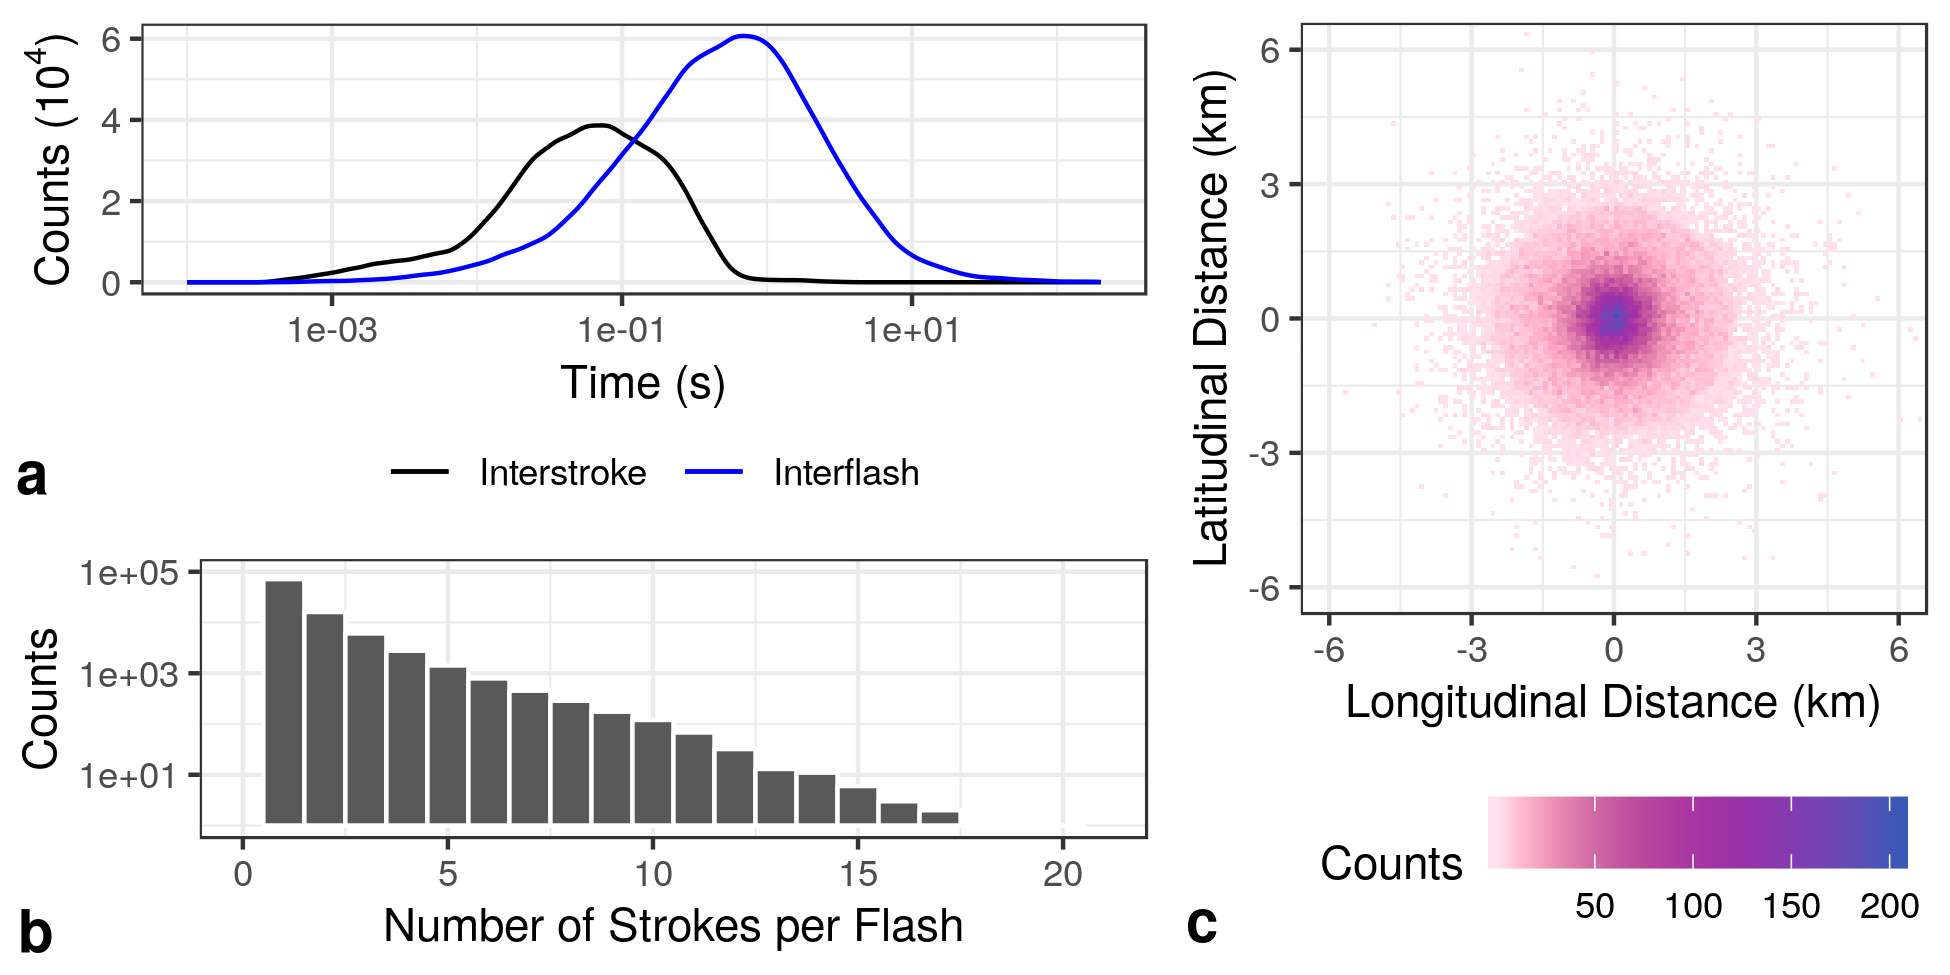
\includegraphics[width=\columnwidth]{../Lightning_Processing/figures/brasildat_flash_stats.png}
		\legend{Fonte: Produzido pela autora.}
	\end{center}
\end{figure}

\section{Outras Bases de Dados}\label{outros_dados}

Para analisar o ambiente sinótico associado a cada caso, dados da reanálise ERA5 e do satélite GOES-16 foram utilizados, descritos a seguir.

\subsection{Reanálise} \label{era5}

O conjunto de dados de reanálise ERA5 \cite{Copernicus2017} é desenvolvido pelo ECMWF (\textit{European Centre for Medium-Range Weather Forecasts}, Centro Europeu para Previsões de Tempo de Médio Alcance) e estão disponíveis publicamente para o período de 2010 a 2-3 meses antes do presente. Este modelo eventualmente substituirá o conjunto de reanálise mais antigo ERA-Interim. A resolução espacial destes dados é de $30\:km$ de cobertura global e 137 níveis verticais, da superfície até $80\:km$ de altura; a resolução temporal é de $1\:h$. Foram usados campos de pressão em superfície, geopotencial, vento e CAPE em diferentes níveis de pressão. Os dados foram obtidos a partir do Armazenamento de Dados Climáticos (\textit{Climate Data Store}, CDS) do Serviço de Mudanças Climáticas Copernicus (\textit{Copernicus Climate Change Service}, CCCS) do ECMWF e processados usando a linguagem Python.

\subsection{Satélite} \label{goes16}

O satélite GOES-16 foi lançado em dezembro de 2016 e está operacional desde 18 de dezembro de 2017. Ele possui 16 canais no principal sensor (ABI - \textit{Advanced Baseline Imager}, Imageador Avançado de Base), além de sensores de raios (GLM - \textit{Geostationary Lightning Mapper}, Mapeador Geoestacionário de Raios) e que medem atividade solar. O modo de escaneamento \textit{Full Disk} (Disco Inteiro) gera uma imagem que inclui a América do Sul continuamente com uma resolução temporal de 5 a 15 minutos e espacial de 0,5 a $2\:km$. Considerando o período de estudo (\autoref{tabela_casos}), 3 dos 5 casos foram analisados com estes dados, usando o canal 13 do ABI, chamado de \textit{"clean"\ longwave infrared window} (janela "limpa" do infravermelho de onda longa), para identificar os sistemas mais intensos e profundos (menor temperatura de brilho). Os dados de nível 2 (convertidos em uma grade latitude-longitudinal e que servem como base para os cálculos de produtos derivados de combinação dos canais) foram obtidos do repositório da NOAA (\textit{National Oceanic and Atmospheric Administration}, Administração Nacional Oceânica e Atmosférica) na AWS (\textit{Amazon Web Services}, Serviços Web da Amazon) \url{https://docs.opendata.aws/noaa-goes16/cics-readme.html} e processados usando a linguagem Python.

% Resultados
\chapter{Resultados}\label{resultados}

Os resultados desta dissertação estão organizados da seguinte forma: uma visão geral de cada caso (\autoref{tabela_casos}) é apresentada através da intensidade da queda de granizo, ciclo de vida e atividade elétrica; dois casos são analisados mais profundamente, incluindo a microfísica e cinemática do sistema convectivo que gerou a queda de granizo.

\section{Intensidade das Tempestades que Geraram Granizo}\label{ciclo_vida}

A \autoref{distribuicao_tamanho} mostra as diferentes distribuições de tamanho de granizo medidas por IAG e LIM (vide \autoref{hailpads}) para cada placa separados por caso (\autoref{tabela_casos}). As plotagens violino (úteis para comparar também os formatos das distribuições) mostram diferenças significativas entre medidas para uma mesma placa além das diferenças entre placas, possivelmente causadas pela subjetividade envolvida na forma em que as cavidades do \textit{hailpad} foram medidas: não houve consenso em relação à definição do diâmetro (eixo maior ou menor, aproximação para um formato esférico, entre outros). Comparando os casos, é possível observar que o caso de 2017-03-14 mostrou menor diversidade de tamanhos de granizo (entre $6$ e $12\:mm$), enquanto que o caso de 2017-11-15 mostrou a maior diversidade considerando os extremos, sendo que este caso teve o maior diâmetro máximo, $22,4\:mm$, com $6,5\:mm$ de diâmetro mínimo.

\begin{figure}[htb]
	\begin{center}
		\caption{Plotagem violino com caixa das distribuições de diâmetro do granizo de diferentes medidas feitas por IAG e LIM separados por caso.} 
		\label{distribuicao_tamanho}
		%		\setcaptionmargin{1cm}
		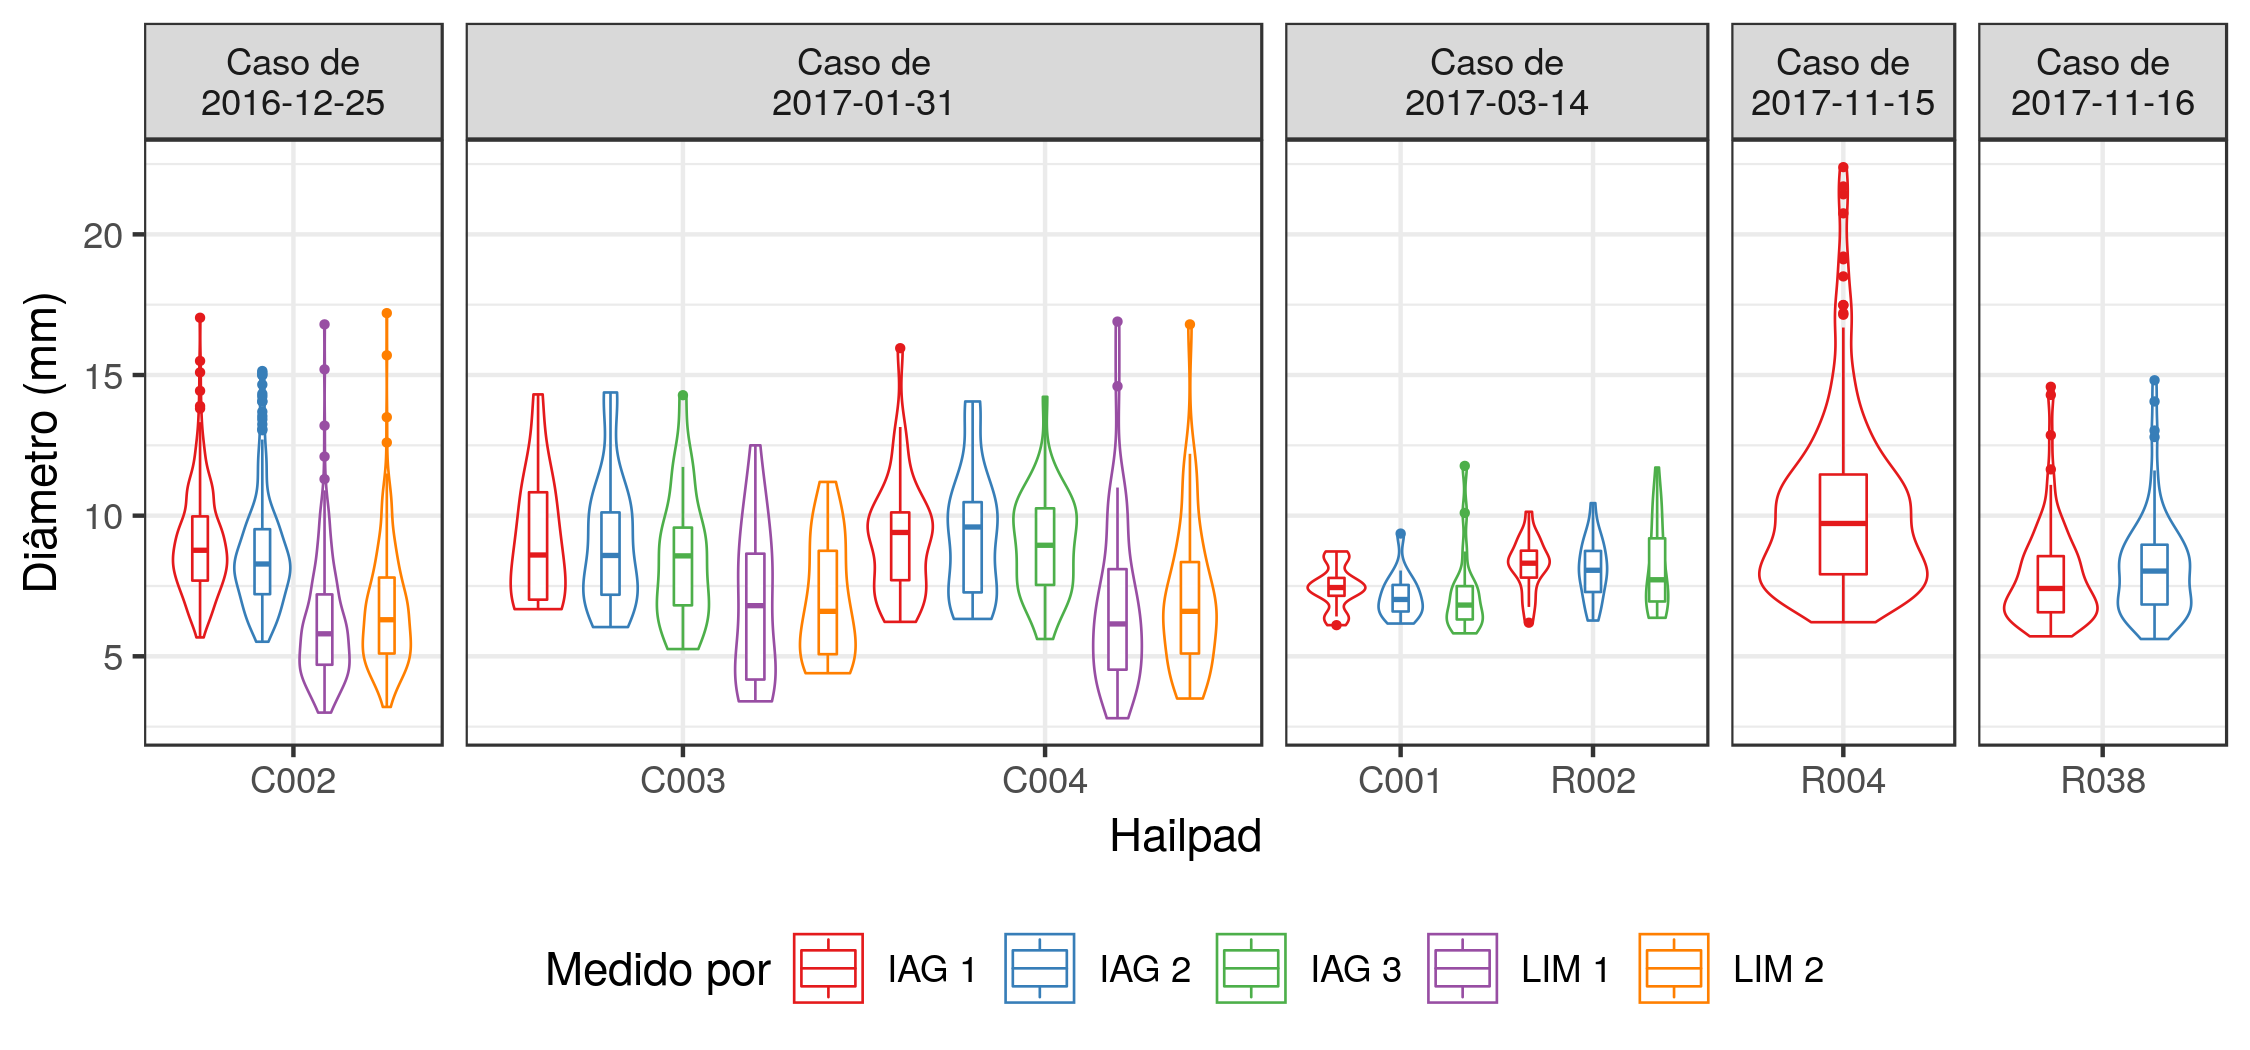
\includegraphics[width=\columnwidth]{../Hailpads_Processing/figures/measures_distribution_ptbr.png}
		\legend{Fonte: Produzido pela autora.}
	\end{center}
\end{figure}

Para os casos com medidas dos dois grupos (2016-12-25 e 2017-01-31), o IAG tende a medir diâmetros maiores que o LIM, o qual mede mais valores extremos principalmente no caso de 2016-12-25 (os diâmetros máximos de IAG 1, LIM 1 e LIM 2 são aproximadamente iguais). Já comparando as placas para um mesmo caso (2017-01-31 e 2017-03-14), as distribuições entre o primeiro e terceiro quartil são similares: no caso de 2017-01-31, por exemplo, as distribuições variaram entre $7$ e $10\:mm$ em todas as medidas do IAG nas duas placas, o que indica que o sistema convectivo que gerou a queda de granizo em um ponto não sofreu mudanças significativas quando gerou a queda de granizo no outro ponto. 

A \autoref{intensidade_anelfatorro} mostra a energia cinética de cada \textit{hailpad} em função do diâmetro do granizo para as escalas ANELFA e TORRO. As barras de erros mais largas em relação ao diâmetro são causadas pelo desvio-padrão maior em placas com maiores diferenças entre cada medida (\autoref{distribuicao_tamanho}). As duas escalas mostram resultados similares entre si, com a maioria das placas relacionadas a casos minimamente intensos porém defasados em relação aos índices mínimos: os diâmetros (máximos ou típicos) são equivalentes a um índice acima da energia cinética correspondente. Isso pode estar relacionado à \autoref{mezeix}, derivada a partir de medições de tempestades na Europa, assim como às próprias escalas que também foram estabelecidas a partir de tempestades no continente europeu: condições locais e sinóticas dessa região são distintas das condições da região de estudo, principalmente comparando sistemas de latitudes médias com tropicais, e essas condições são importantes na formação de granizo. \citeonline{Sanchez2009}, ao comparar distribuições de tamanho de granizo em três países com redes de \textit{hailpads}, mostram que podem ocorrer diferenças nos parâmetros característicos mesmo em localidades geograficamente próximas, diferença que pode ser propagada facilmente na estimativa da energia cinética dos \textit{hailpads}.

\begin{figure}[htb]
	\begin{center}
		\caption{Energia cinética do \textit{hailpad} em função do diâmetro do granizo considerando as escalas ANELFA e TORRO, com os índices de A0 a A2 e de H0 a H2 (\autoref{tabela_escalas}) indicados.} 
		\label{intensidade_anelfatorro}
		%		\setcaptionmargin{1cm}
		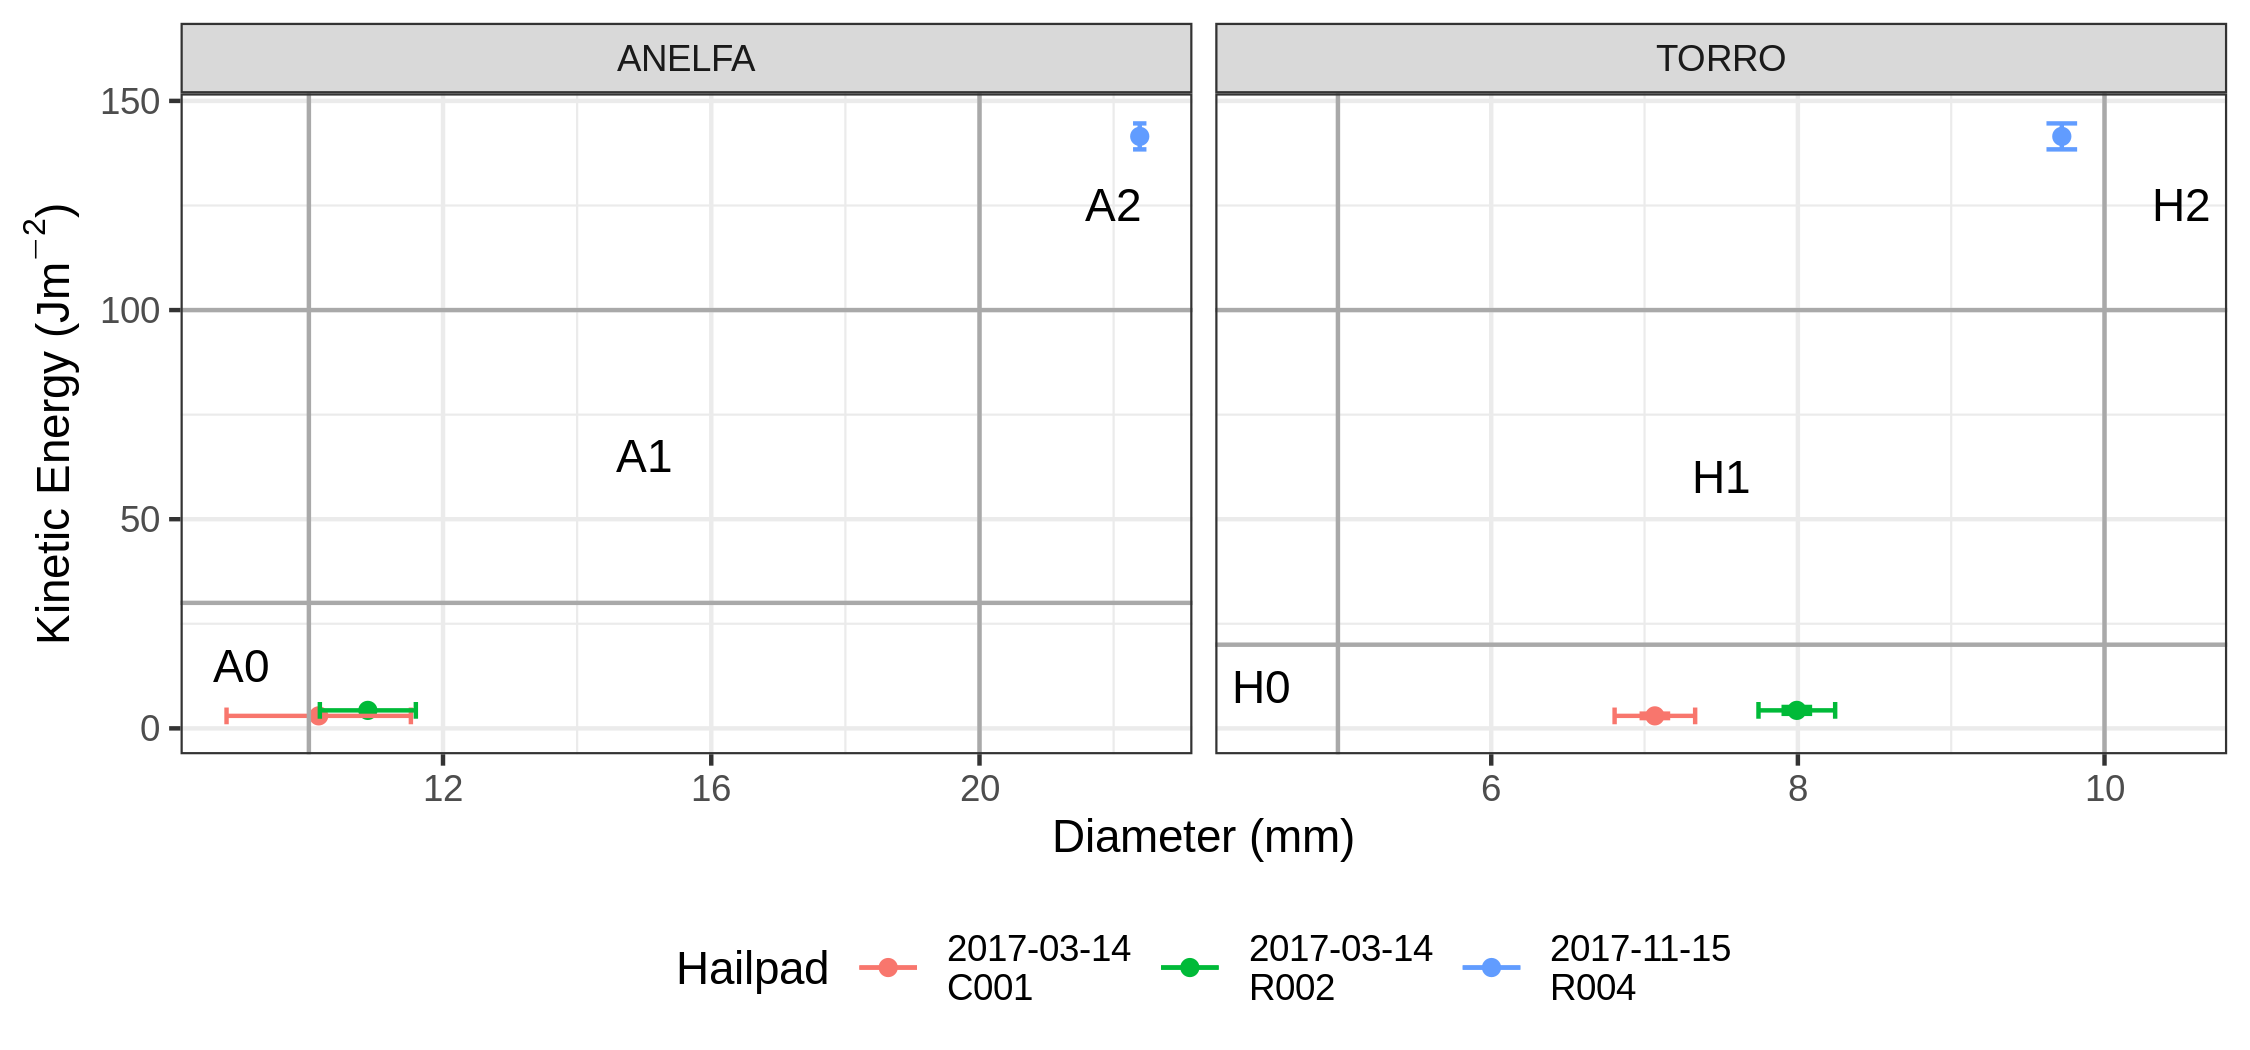
\includegraphics[width=\columnwidth]{../Hailpads_Processing/figures/data_anelfa_torro_ptbr.png}
		\legend{Fonte: Produzido pela autora.}
		\nota{A escala ANELFA leva em conta o diâmetro máximo medido no \textit{hailpad}, enquanto que a escala TORRO leva em conta o diâmetro típico da distribuição medida no \textit{hailpad}.}
	\end{center}
\end{figure}

Dentro da escala ANELFA (painel esquerdo da \autoref{intensidade_anelfatorro}), o caso de 2017-11-15 foi considerado o mais intenso, dentro do índice A2 (danos sérios a vegetais e árvores - foram reportados danos à plantações próximas da localização do \textit{hailpad} em Indaiatuba), com o caso de 2016-12-25 sendo o segundo mais intenso, dentro do índice A1 (danos à vinhas e pomares). No caso de 2017-03-14, com mais de um \textit{hailpad}, a queda de granizo em Indaiatuba (placa R002) foi ligeiramente mais intensa do que em Cosmópolis (placa C004) (diferença de $1\:mm$ no diâmetro máximo e de cerca de $2\:Jm^{-2}$ de energia cinética). Dentro da escala TORRO (painel direito da \autoref{intensidade_anelfatorro}) os resultados foram similares, com o caso de 2017-11-15 sendo o mais intenso também mas ligeiramente fora do índice H2 (tempestade significante) e o caso de 2016-12-25 sendo o segundo mais intenso, dentro do índice H1 (tempestade potencialmente prejudicial). A queda de granizo em Indaiatuba no caso de 2017-03-14 também foi ligeiramente mais intensa do que em Cosmópolis.

A \autoref{painel_ciclo} mostra a evolução temporal da refletividade máxima em $3\:km$ de altura (a), tamanho do sistema convectivo (b) e taxa de raios (c), enquanto que a \autoref{tabela_resumo_casos} mostra um panorama geral das características físicas relacionadas ao ciclo de vida dos casos em análise, rastreados usando o algoritmo ForTraCC-Radar (\autoref{radar}). De forma geral, a queda de granizo ocorreu dentro da fase de maturação dos sistemas convectivos, com refletividade acima de $60\:dBZ$, área em relativo crescimento e intensa atividade elétrica. O caso de 2017-01-31 foi o com menor tempo de vida ($0,5\:h$), área máxima ($69\:km^2$) e quantidade de raios ($3\:flashes$), mas não teve o menor tamanho de granizo: o caso de 2016-12-25 teve o menor granizo médio, enquanto que o caso de 2017-03-14 teve o menor granizo máximo (e granizo médio ligeiramente maior). O mesmo caso de 2017-03-14 foi o com maior tempo de vida ($6,2\:h$), refletividade máxima ($70\:dBZ$) e quantidade e taxa máxima de raios (10525 (2576) $flashes$ IC (CG), com taxa máxima de 107 (31) $flashes\:min^{-1}$ IC (CG)). Outro caso a ser destacado é o de 2017-11-15, com tempo de vida curto ($2,2\:h$), área máxima pequena ($253\:m^2$) e pouca quantidade de raios (menos de 100 $flashes$ somando IC e CG, taxa máxima abaixo de $5\:flashes\:min^{-1}$), mas que mostrou granizos acima de $10\:mm$ em média e granizo máximo de $22,4\:mm$. Considerando o papel do granizo na formação de raios (\autoref{granizo_eletrificacao}), é de se esperar uma relação direta entre mudança da atividade elétrica e queda de granizo (\autoref{painel_ciclo}c), porém ela não foi consistente em todos os casos: em 2016-12-25, 2017-03-14 e 2017-11-15 há um ligeiro aumento da atividade elétrica (principalmente raios IC) até 30 minutos antes da queda de granizo, enquanto que em 2017-01-31 não há raios suficientes para determinar aumento ou diminuição da atividade elétrica, e em 2017-11-16 há um aumento da atividade elétrica depois da queda de granizo.

\begin{figure}[htb]
	\begin{center}
		\caption{Evolução temporal da refletividade máxima em $3\:km$ (a), tamanho do sistema (b) e taxa de \textit{flashes} CG e IC (c). As linhas pontilhadas indicam o momento aproximado em que houve a queda de granizo medida no \textit{hailpad}.} 
		\label{painel_ciclo}
		%		\setcaptionmargin{1cm}
		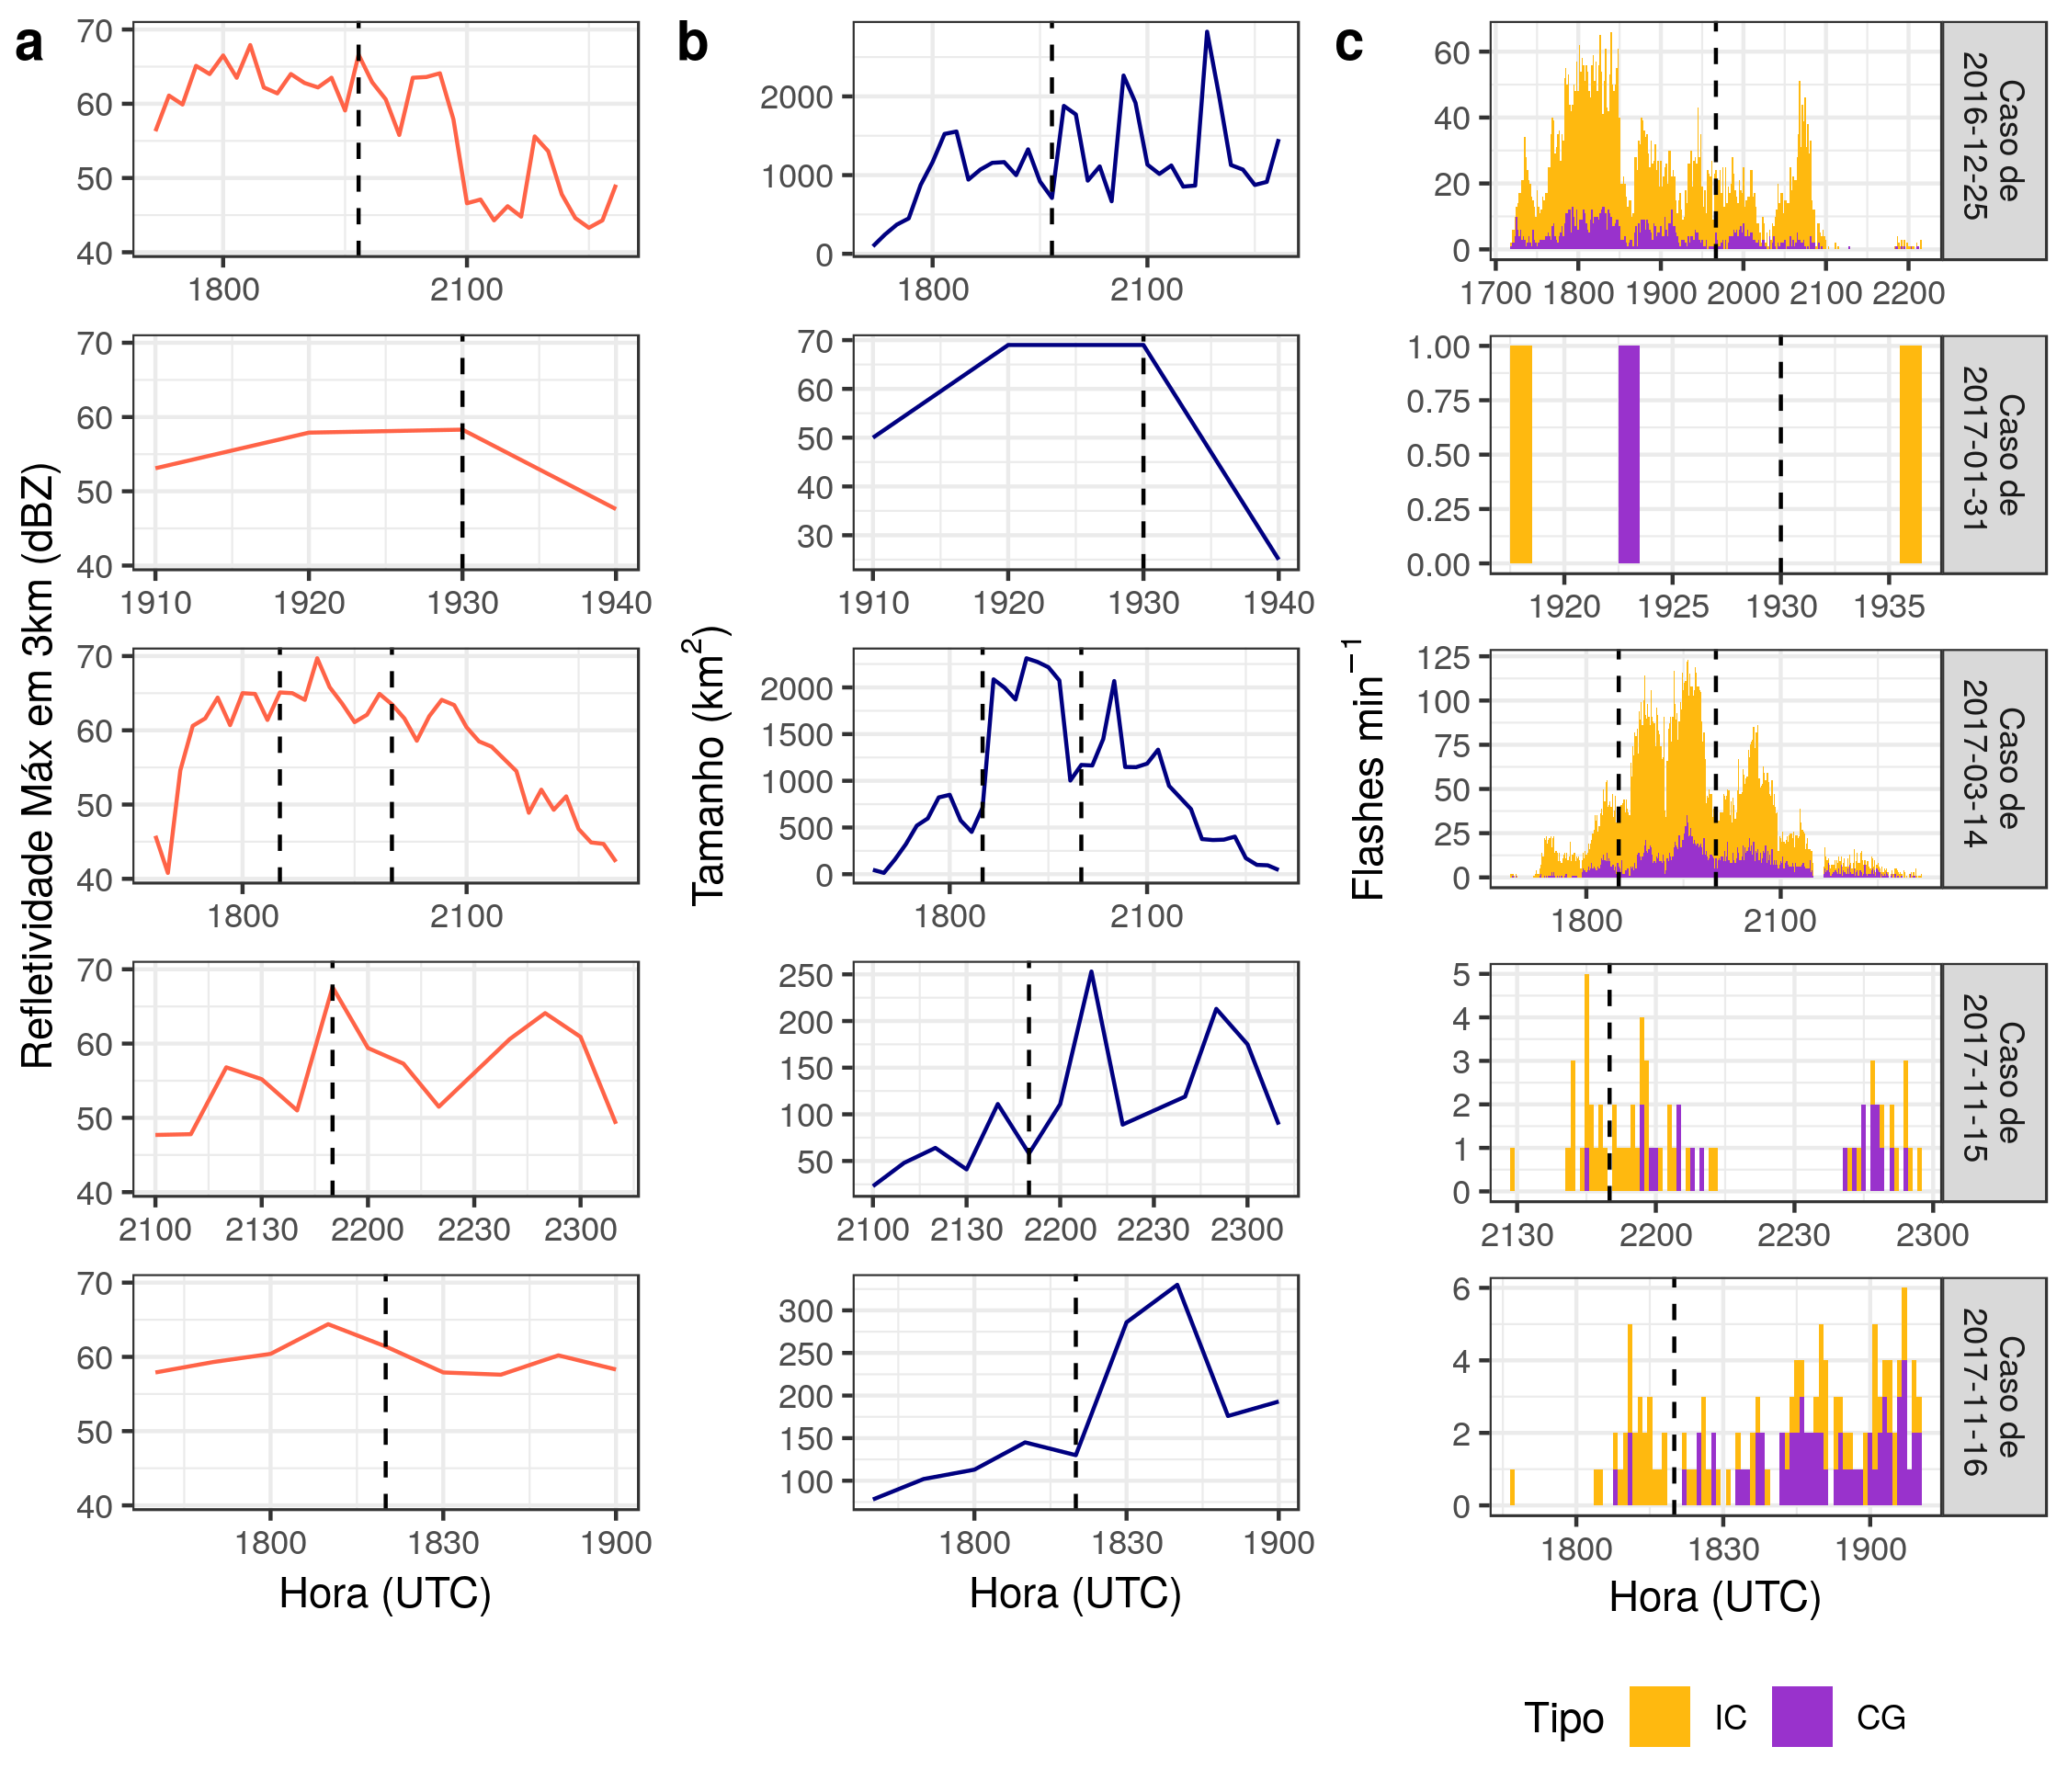
\includegraphics[width=0.99\columnwidth]{../General_Processing/figures/cases_dbz_size_lightning_ptbr.png}
		\legend{Fonte: Produzido pela autora.}
	\end{center}
\end{figure}

\begin{table}[htb]
	\IBGEtab{%
		\caption{Resumo das principais características físicas e elétricas dos casos analisados}%
		\label{tabela_resumo_casos}
	}{%
		\begin{tabularx}{\textwidth}{cY>{\hsize=1.5\hsize}Y>{\hsize=1.5\hsize}Y>{\hsize=1.5\hsize}Y>{\hsize=1.5\hsize}Y>{\hsize=0.75\hsize}Y>{\hsize=0.75\hsize}YYY}
			\toprule
			Caso & Tempo de Vida ($h$) & Z Máximo em $3\:km$ ($dBZ$) & Área Máxima ($km^2$) & Granizo Médio ($mm$) & Granizo Máximo ($mm$) & \multicolumn{2}{>{\hsize=2\hsize}Y}{Total de Raios ($flashes$)} & \multicolumn{2}{>{\hsize=2\hsize}Y}{Taxa Máxima de Raios ($flashes\ min^{-1}$)} \\
			\cmidrule(l){7-10}
			 & & & & & & IC & CG & IC & CG \\
			\midrule
			2016-12-25 & $5,7$ & $67,9$ & $2822$ & $7,6$ & $17,2$ & $13130$ & $2260$ & $104$ & $26$ \\
			\midrule 
			2017-01-31 & $0,5$ & $58,3$ & $69$ & $8,2$ & $16,9$ & $4$ & $4$ & $1$ & $1$ \\
			\midrule 
			2017-03-14 & $6,2$ & $69,7$ & $2312$ & $7,8$ & $11,8$ & $15131$ & $4185$ & $125$ & $33$ \\
			\midrule 
			2017-11-15 & $2,2$ & $67,6$ & $253$ & $10,3$ & $22,4$ & $86$ & $29$ & $8$ & $3$ \\
			\midrule 
			2017-11-16 & $1,3$ & $64,4$ & $330$ & $8$ & $14,8$ & $528$ & $227$ & $19$ & $8$ \\
			\bottomrule
		\end{tabularx}%
	}{%
		\fonte{Produzido pela autora.}%
	}
\end{table}


A partir dos resultados descritos nesta seção, dois casos foram escolhidos para uma análise mais detalhada:

\begin{alineas}
	\item \textbf{2017-03-14}: Classificado como tempestade com queda de granizo de baixa intensidade, este caso teve alta atividade elétrica durante seu longo ciclo de vida, gerando queda de granizo em dois pontos diferentes. Os dois momentos em que houve queda de granizo serão comparados em relação à estrutura e cinemática da nuvem;
	\item \textbf{2017-11-15}: Classificado com tempestade com queda de granizo de intensidade significativa, este caso teve baixa atividade elétrica, o que não é esperado em uma tempestade com produção de granizo suficiente para cair no solo com tamanho considerável. A microfísica e cinemática desta tempestade com ciclo de vida mais curto ajudará a explicar esse comportamento.
\end{alineas}

\section{Estudos de Caso}\label{estudo_casos}

Os estudos dos casos de 2017-03-14 e 2017-11-15 estão descritos a seguir, focando: no ambiente sinótico e termodinâmico em que os sistemas convectivos se formaram; na atividade elétrica ao longo dos ciclos de vida; na microfísica através da estrutura vertical da convecção quando houve queda de granizo e; na cinemática, observando os campos de vento derivado por Multi-Doppler antes e durante a queda de granizo.

\subsection{Caso de 2017-03-14}

\subsubsection{Ambiente Sinótico e Termodinâmico}\label{sinotica_201703014}

A influência de uma frente fria no litoral de São Paulo e do Rio de Janeiro durante a madrugada foi determinante para o disparo de sistemas convectivos no estado de São Paulo durante a tarde. O sistema frontal em si se deslocou para o Oceano Atlântico ao longo do dia - às 1200 UTC (Figura\autoref{era5_2017031412_jets}), o sistema está à leste de $30^{\circ}W$ - mas favoreceu a convergência de umidade na região de estudo (não mostrado). Às 1200 UTC, a radiossondagem (\autoref{sondagem_20170314}) mostra uma camada úmida entre a superfície e $600\:hPa$, mas com CAPE (\textit{Convective Available Potential Energy}, Energia Potencial Disponível para Convecção) nulo e pouco cisalhamento (mesma condição no resto do estado, como mostra a Figura\autoref{era5_2017031412_cape}). Já às 1500 UTC (Figura\autoref{era5_2017031415_cape}), o potencial para convecção (CAPE entre 500 e $1500\:J\:kg^{-1}$) e o cisalhamento (de até 10 nós) aumentaram, disparando sistemas convectivos no centro do estado de São Paulo. As imagens de satélite da \autoref{goes16_sp_20170314} mostram a propagação e intensificação de sistemas convectivos com topos de até $-75^{\circ}C$ de temperatura de brilho em alguns pontos na região de estudo aproximadamente às 1800 (a) e 2000 UTC (b), o que inclui o sistema que causou queda de granizo em Cosmópolis e Indaiatuba. 

\begin{figure}[hp]
	\begin{center}
		\caption{Campos da reanálise do ERA5 em 2017-03-14: Pressão ao nível médio do mar, espessura entre $1000$ e $500\:hPa$ e velocidade do vento em $250\:hPa$ às 1200 UTC (a); altura geopotencial em $850\:hPa$, cisalhamento do vento entre $1000$ e $500\:hPa$ e CAPE em superfície às 1200 (b) e 1500 UTC, no domínio do estado de São Paulo (c).} 
		\label{era5_20170314_main}
		\subfloat[]{\includegraphics[width=0.495\columnwidth]{../Reanalysis_Processing/figures/ERA5_SA_sfc-jets_201703141200_ptbr.png}
			\label{era5_2017031412_jets}}
		\subfloat[]{\includegraphics[width=0.505\columnwidth]{../Reanalysis_Processing/figures/ERA5_SA_cape-shear_201703141200_ptbr.png}
			\label{era5_2017031412_cape}} \\
		\subfloat[]{\includegraphics[width=0.505\columnwidth]{../Reanalysis_Processing/figures/ERA5_SP-BR_cape-shear_201703141500_ptbr.png}
			\label{era5_2017031415_cape}} \\
		\legend{Fonte: Produzido pela autora.}
	\end{center}
\end{figure}

\begin{figure}[hp]
	\begin{center}
		\caption{Plotagem Skew-T Log-P da radiossondagem do Campo de Marte (SP) com hodógrafa do vento e índices CAPE e CIN em 2017-03-14 1200 UTC.} 
		\label{sondagem_20170314}
		%		\setcaptionmargin{1cm}
		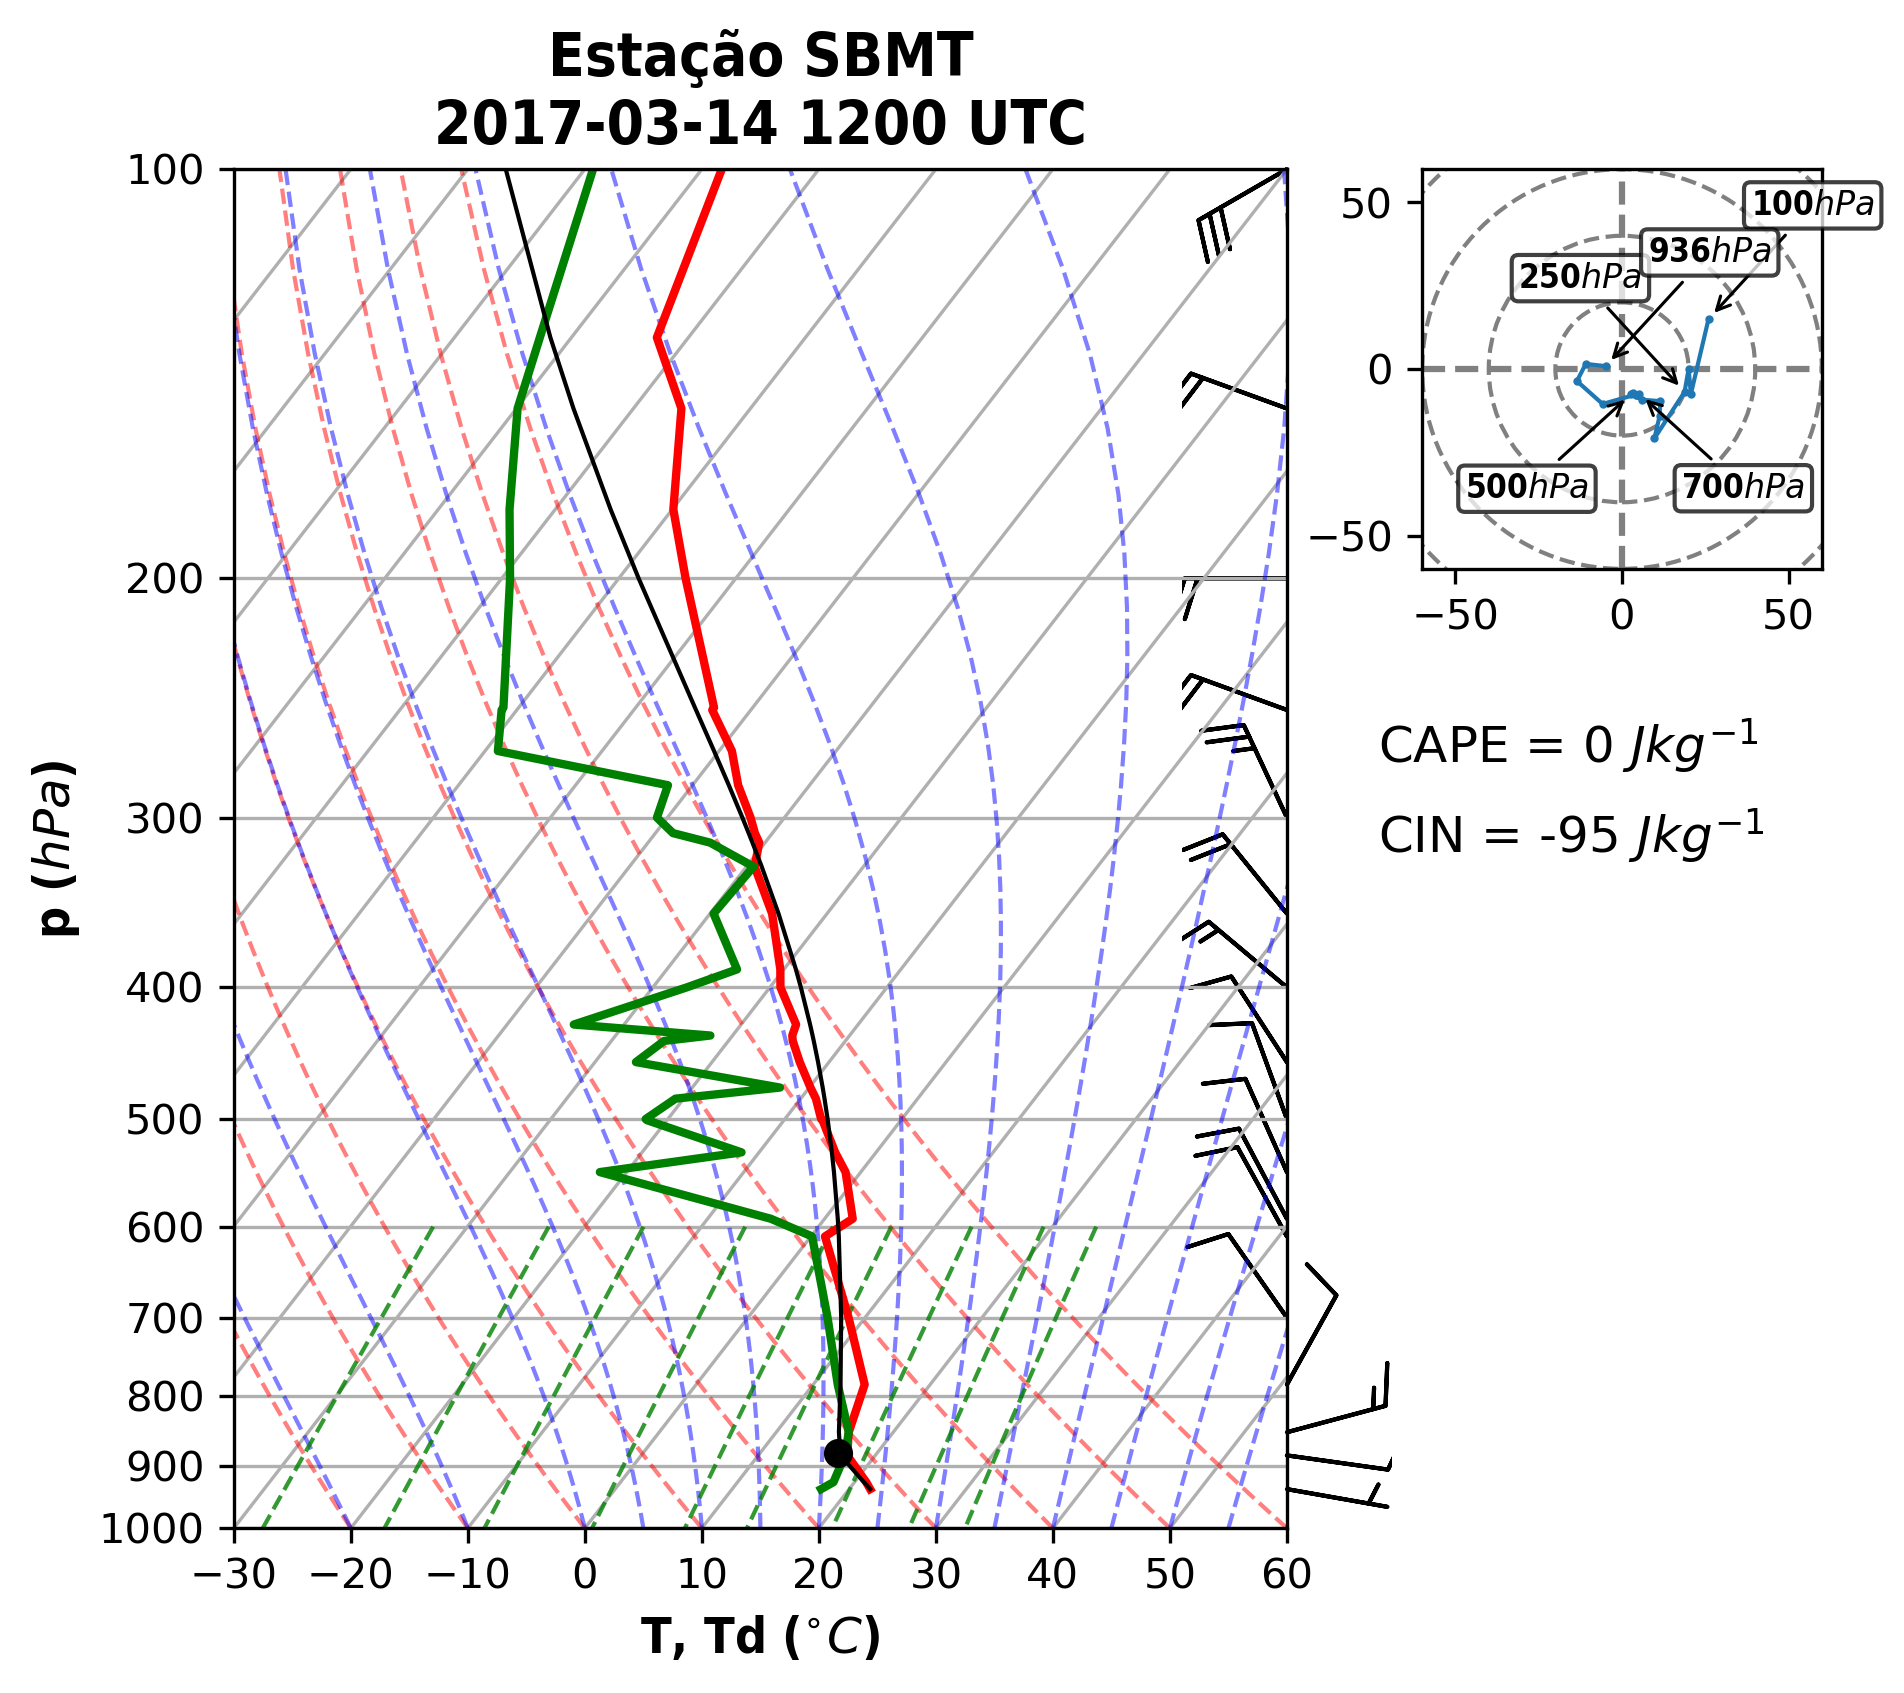
\includegraphics[width=0.75\columnwidth]{../Sounding_Processing/figures/sounding_SBMT2017031412UTC_ptbr.png}
		\legend{Fonte: Produzido pela autora.}
	\end{center}
\end{figure}

%\begin{figure}[htb]
%	\begin{center}
%		\caption{Imagem de satélite do canal 13 do GOES-16 mostrando a temperatura de brilho do topo das nuvens na América do Sul em 2017-03-14 1751 UTC.} 
%		\label{goes16_sa_20170314}
%		%		\setcaptionmargin{1cm}
%		\includegraphics[width=0.75\columnwidth]{../Satellite_Processing/figures/Band_13/GOES16_B13_SA_SD201703141751.png}
%		\legend{Fonte: Produzido pela autora.}
%	\end{center}
%\end{figure}
%
\begin{figure}[hp]
	\begin{center}
		\caption{Imagem de satélite do canal 13 do GOES-16 mostrando a temperatura de brilho do topo das nuvens no estado de São Paulo em 2017-03-14 1751 (a) e 1951 UTC (b).} 
		\label{goes16_sp_20170314}
		\subfloat[]{\includegraphics[width=0.5\columnwidth]{../Satellite_Processing/figures/Band_13/GOES16_B13_SP-BR_SD201703141751_ptbr.png}
			\label{goes16_sp_20170314_1}}
		\subfloat[]{\includegraphics[width=0.5\columnwidth]{../Satellite_Processing/figures/Band_13/GOES16_B13_SP-BR_SD201703141951_ptbr.png}
			\label{goes16_sp_20170314_2}} \\
		\legend{Fonte: Produzido pela autora.}
	\end{center}
\end{figure}

\subsubsection{Eletrificação}\label{elec_201703014}

A \autoref{track_flashes_20170314} mostra a localização do sistema ao longo do ciclo de vida e dos \textit{flashes} associados a ele. Como já mostrado (\autoref{painel_ciclo}, \autoref{tabela_casos}), este caso teve um longo ciclo de vida com intensa atividade elétrica - a taxa de \textit{flashes} chega a um máximo (107 (31) $flashes\:\:min^{-1}$ IC (CG)) após a queda de granizo em Cosmópolis e diminui antes do evento em Indaiatuba. O sistema convectivo se deslocou por toda a RMC e regiões vizinhas na direção sudoeste, com fusões e separações com sistemas menores. Os \textit{flashes} IC e CG ocorreram principalmente dentro da RMC durante todo o ciclo de vida, com cerca de 5 vezes mais \textit{flashes} IC (10525) do que CG (2576).

\begin{figure}[htb]
	\begin{center}
		\caption{Rastreamento (a) e localização dos \textit{flashes} IC e CG (b) do sistema convectivo responsável pelas quedas de granizo em Cosmópolis e Indaiatuba em 2017-03-14. Os triângulos pretos indicam a localização dos \textit{hailpads}.} 
		\label{track_flashes_20170314}
		%		\setcaptionmargin{1cm}
		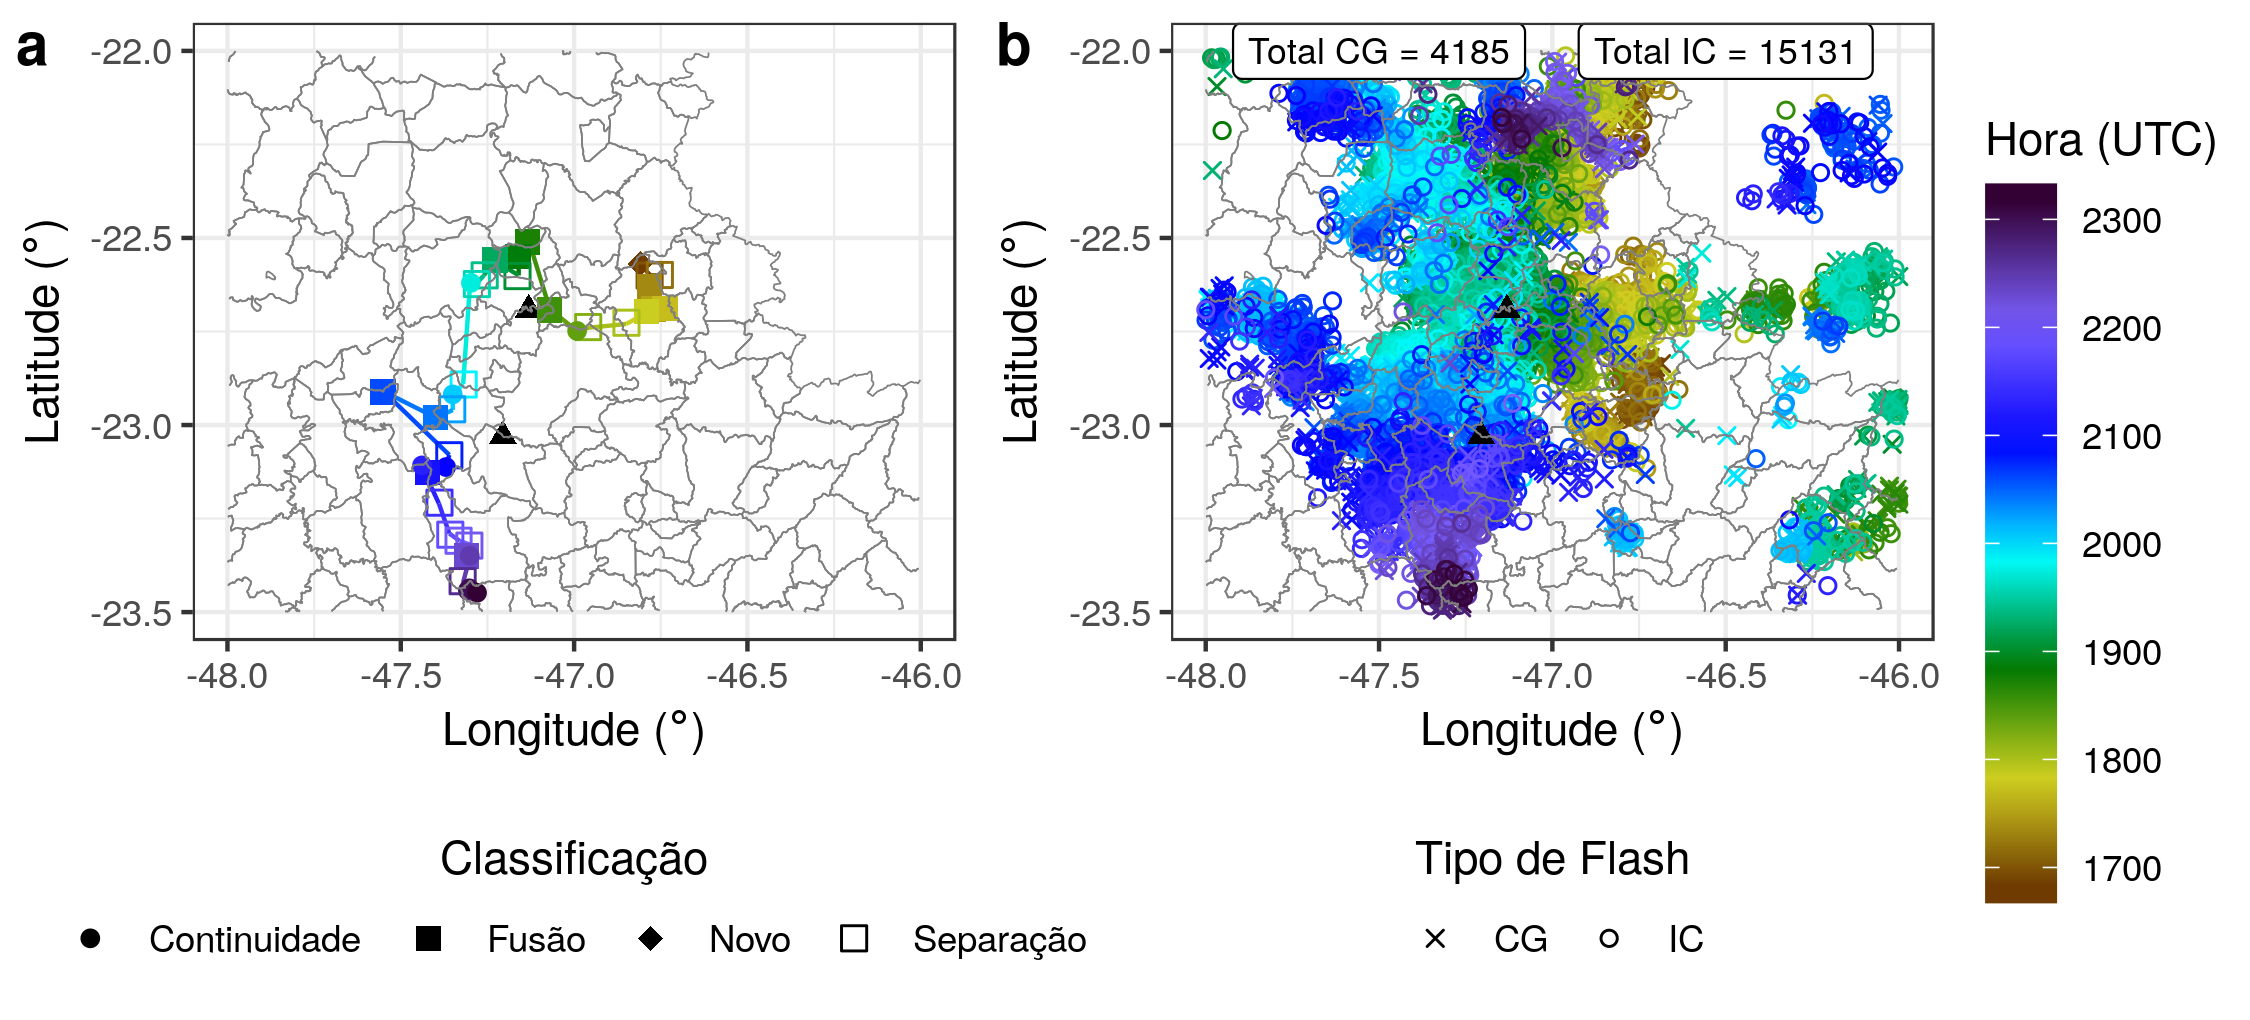
\includegraphics[width=\columnwidth]{../General_Processing/figures/track_flashes_20170314_ptbr.png}
		\legend{Fonte: Produzido pela autora.}
	\end{center}
\end{figure}

A \autoref{dbz_flashes_20170314_1} mostra os campos de refletividade (a) e \textit{flashes} IC (b) e CG (c) para o caso de 2017-03-14 antes, durante e depois da queda de granizo em Cosmópolis. O núcleo convectivo mais próximo à localização do \textit{hailpad} está embebido em um sistema multicelular que abrange boa parte do norte da RMC e passa por um processo de fusão com outros núcleos convectivos no período mostrado. A densidade de raios é maior (acima de $60$ ($10$) \textit{flashes} IC (CG)) ligeiramente à leste (sul) da localização do \textit{hailpad} antes (depois) da queda de granizo, associado aos núcleos mais intensos (refletividade acima de $60\:dBZ$). 

\begin{figure}[htb]
	\centering
	\caption{Campos de refletividade (a) e \textit{flashes} IC (b) e CG (c) acumulados em 10 minutos do sistema convectivo (delimitado pela linha preta) responsável pela queda de granizo em Cosmópolis em 2017-03-14. O triângulo preto indica a localização do \textit{hailpad}. Linhas contínuas demarcam os limites dos municípios do Estado de São Paulo.} 
	\label{dbz_flashes_20170314_1}
	%\vspace{-5pt}
	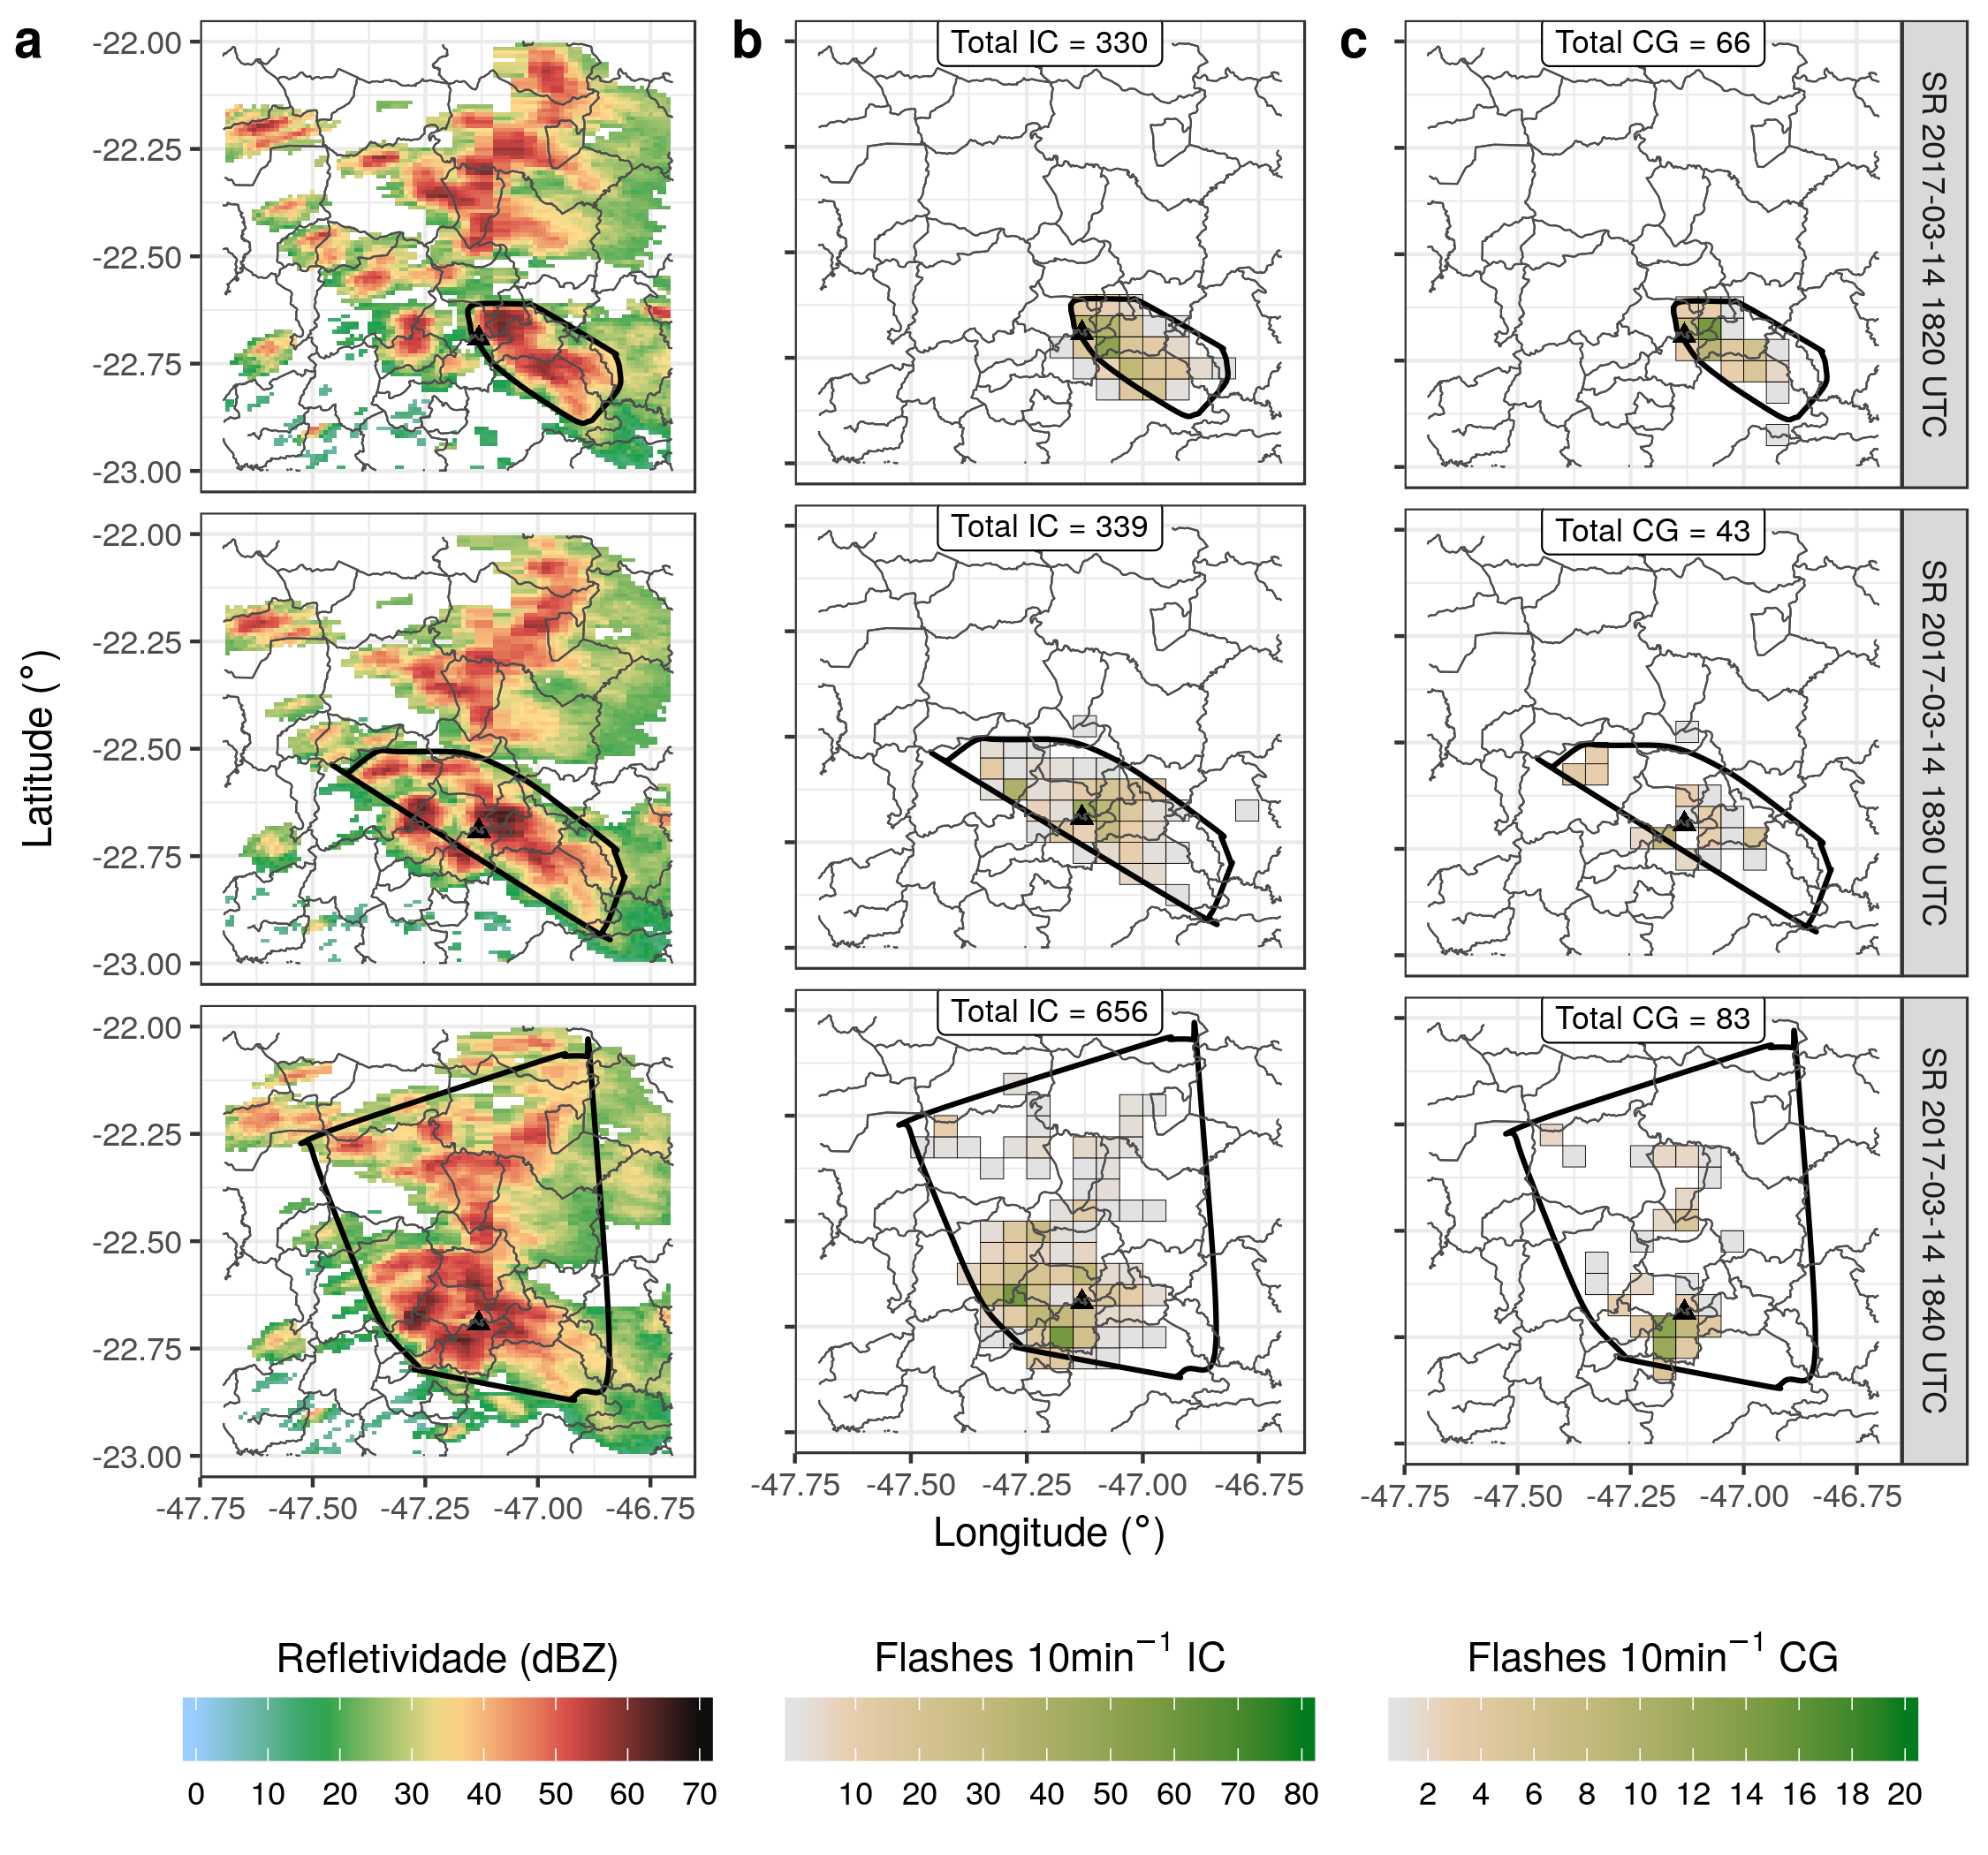
\includegraphics[width=0.99\columnwidth]{../General_Processing/figures/clusters_flashes_2017-03-14_1830_ptbr.png} \\
	\legend{Fonte: Produzido pela autora.}
\end{figure}

Depois da queda de granizo em Cosmópolis, o sistema convectivo se separou em diversos sistemas menores (não mostrado); o maior desses sistemas se intensificou e prosseguiu na direção sul/sudeste (\autoref{track_flashes_20170314}a), causando a queda de granizo em Indaiatuba (\autoref{dbz_flashes_20170314_2}). O núcleo convectivo mais próximo à localização do \textit{hailpad} moveu-se lentamente no período mostrado, enquanto o resto do sistema à oeste se fundiu com núcleos convectivos pequenos. A maior densidade de raios (acima de $40$ ($10$) \textit{flashes} IC (CG)) está associada ao núcleo mais intenso (refletividade acima de $55\:dBZ$) ligeiramente à leste do \textit{hailpad}; a quantidade de raios aumentou após a queda de granizo em Indaiatuba. 

\begin{figure}[htb]
	\centering
	\caption{Campos de refletividade (CAPPI em $3\:km$ do radar de São Roque) (a) e \textit{flashes} IC (b) e CG (c) acumulados em 10 minutos do sistema convectivo (delimitado pela linha preta) responsável pela queda de granizo em Indaiatuba em 2017-03-14. O triângulo preto indica a localização do \textit{hailpad}. Linhas contínuas demarcam os limites dos municípios do Estado de São Paulo.} 
	\label{dbz_flashes_20170314_2}
	%\vspace{-5pt}
	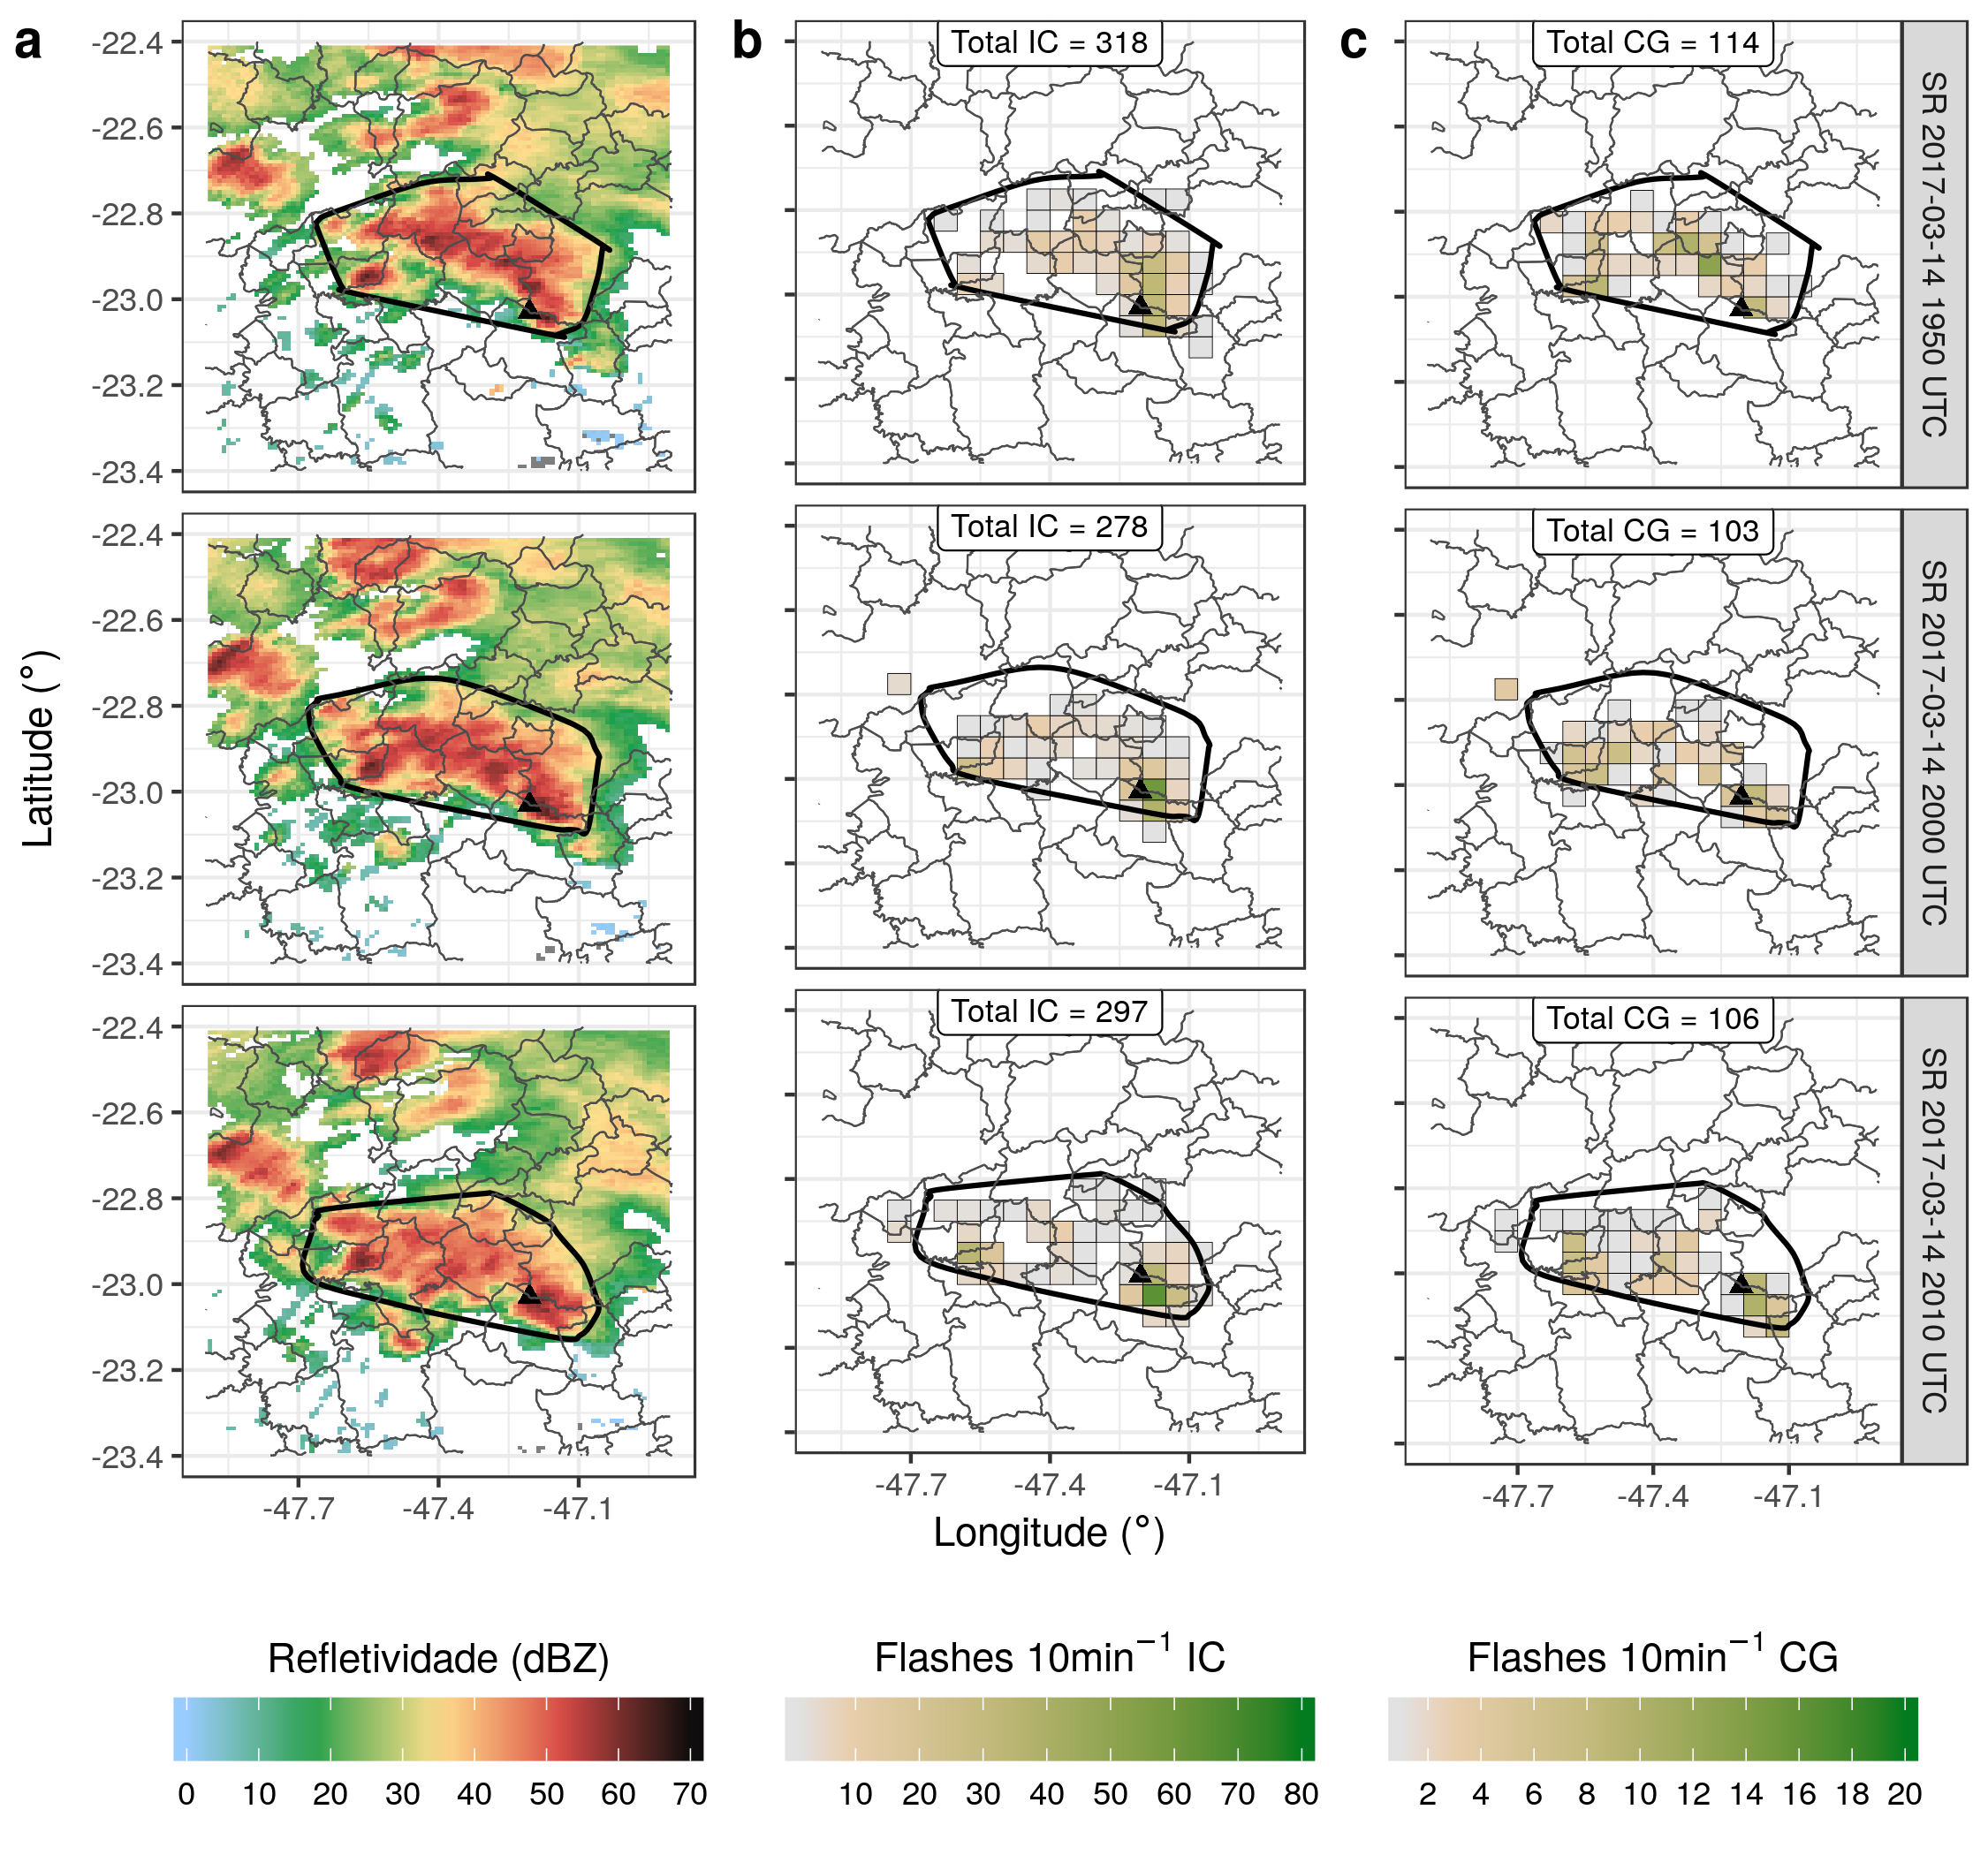
\includegraphics[width=0.99\columnwidth]{../General_Processing/figures/clusters_flashes_2017-03-14_2000_ptbr.png} \\
	\legend{Fonte: Produzido pela autora.}
\end{figure}

\subsubsection{Microfísica}\label{micro_201703014}

A \autoref{radar_20170314_1} mostra os campos de refletividade e variáveis polarimétricas refletividade diferencial, fase diferencial específica e coeficiente de correlação do radar da FCTH para o caso de 2017-03-14, no momento mais próximo da queda de granizo em Cosmópolis; a \autoref{radar_derived_20170314_1} mostra a identificação de hidrometeoros e massas de água líquida e gelo calculadas a partir dos campos de radar. O núcleo convectivo que causou a queda de granizo é formado por uma região de refletividade acima de $50\:dBZ$ de cerca de $10\:km$ de extensão horizontal e vertical (da superfície até a isoterma de $-40\:^{\circ}C$) (\autoref{radar_20170314_1}a). Os valores abaixo de 0,9 de coeficiente de correlação entre a superfície e a isoterma de $0\:^{\circ}C$ (\autoref{radar_20170314_1}d) confirmam a presença de granizo ou a coexistência de granizo e chuva em vez de apenas chuva (também associado a altas refletividades) nessa região. Valores negativos de fase diferencial específica acima de $16\:km$ de altura indicam a presença de gelo vertical. No núcleo convectivo imediatamente à esquerda, observa-se valores relativamente altos de fase diferencial específica (cerca de $1\:^\circ\:km^{-1}$) logo acima da isoterma de $0\:^{\circ}C$, indicando a presença de água líquida superesfriada, associado a refletividade diferencial positiva (entre 1 e $2\:dB$) até $-40\:^{\circ}C$. Esses resultados corroboram com as características de sistemas convectivos eletricamente ativos reportados em outros estudos na região \cite{Mattos2015, Mattos2016a, Mattos2017}.

Os campos derivados das variáveis polarimétricas são acurados na classificação de granizo no núcleo convectivo responsável pela queda de granizo em Cosmópolis (\autoref{radar_derived_20170314_1}a) e na massa de gelo associada (que chegou a cerca de $15\:gm^{-3}$ abaixo de $2\:km$, \autoref{radar_derived_20170314_1}c), mas apresenta problemas associados à estratégia do radar. A classificação de hidrometeoros é muito similar ao campo de refletividade (o que é esperado já que o algoritmo dá maior peso à essa variável e à temperatura, vide \autoref{hid}), com regiões de refletividade acima de $50\:dBZ$ classificadas como granizo, entre 40 e $50\:dBZ$ como graupel de densidade alta (DA) e entre 30 e $40\:dBZ$ como graupel de densidade baixa (DB); para refletividades abaixo de $30\:dBZ$, a classificação de cristais de gelo e agregados ocorre mesmo abaixo da isoterma de $0\:^{\circ}C$ (gelo vertical em $1\:km$ de altura em $\ang{22.79}S$, $\ang{47.24}W$, por exemplo), condição muito difícil de ser encontrada em nuvens frias de tempestades tropicais. O campo de massa de água líquida (\autoref{radar_derived_20170314_1}b) apresenta o mesmo problema, onde é possível observar massa de $1\:gm^{-3}$ acima da isoterma de $-40\:^{\circ}C$ no núcleo associado à queda de granizo; mesmo sendo um valor baixo, é difícil encontrar água na forma líquida em regiões com temperaturas tão baixas. A estratégia desse radar (Figura\autoref{estrategia_cth}) é essencial para entender esse problema: nessa região (à aproximadamente $160\:km$ do radar), a primeira elevação faz uma varredura entre 3 e $6\:km$ de altura, ou seja, entre possivelmente a região de fase quente e mista (acima da isoterma de $0\:^{\circ}C$) da nuvem, o que prejudica tanto a interpolação de dados volumétricos para uma grade uniforme (pois os níveis abaixo de $3\:km$ são aproximações do que foi medido em $3\:km$) quanto a identificação de hidrometeoros (pois esses dados interpolados representam uma mistura cada vez maior de hidrometeoros nos níveis mais baixos, tornando a classificação imprecisa).

\begin{figure}[hp]
	\centering
	\caption{Corte horizontal em $3\:km$ de altura e vertical entre os pontos A e B de campos do radar da FCTH em 2017-03-14 1827 UTC, no momento mais próximo da queda de granizo em Cosmópolis: Refletividade corrigida (a) e diferencial (b), fase diferencial específica (c) e coeficiente de correlação (d). O 'x' indica a localização do \textit{hailpad} e as isotermas de $0$ e $-40^{\circ}C$ foram definidas a partir da radiossondagem de SBMT. Linhas contínuas demarcam os limites dos municípios do Estado de São Paulo.}
	\label{radar_20170314_1}
	\vspace{-5pt}
	\includegraphics[width=\columnwidth]{../Radar_Processing/figures/ppis/classification/FCTH Refletividade Corrigida 2017-03-14 1827 UTC.png} \\
	\vspace{-5pt}
	\includegraphics[width=\columnwidth]{../Radar_Processing/figures/ppis/classification/FCTH Refletividade Diferencial 2017-03-14 1827 UTC.png} \\
	\vspace{-5pt}
	\includegraphics[width=\columnwidth]{../Radar_Processing/figures/ppis/classification/FCTH Fase Diferencial Específica 2017-03-14 1827 UTC.png} \\
	\vspace{-5pt}
	\includegraphics[width=\columnwidth]{../Radar_Processing/figures/ppis/classification/FCTH Razão de Correlação Cruzada 2017-03-14 1827 UTC.png} \\
	\legend{Fonte: Produzido pela autora.}
\end{figure}

\begin{figure}[htb]
	\centering
	\caption{Corte horizontal em $3\:km$ de altura e vertical entre os pontos A e B de campos derivados do radar da FCTH em 2017-03-14 1827 UTC, no momento mais próximo da queda de granizo em Cosmópolis: Identificação de hidrometeoros (a) e massas de água líquida (b) e gelo (c). O 'x' indica a localização do \textit{hailpad} e as isotermas de $0$ e $-40^{\circ}C$ foram definidas a partir da radiossondagem de SBMT. Linhas contínuas demarcam os limites dos municípios do Estado de São Paulo.} 
	\label{radar_derived_20170314_1}
	\vspace{-5pt}
	\includegraphics[width=\columnwidth]{../Radar_Processing/figures/ppis/classification/FCTH IDs de Hidrometeoros 2017-03-14 1827 UTC.png} \\
	\vspace{-5pt}
	\includegraphics[width=\columnwidth]{../Radar_Processing/figures/ppis/classification/FCTH Massa de Água Líquida 2017-03-14 1827 UTC.png} \\
	\vspace{-5pt}
	\includegraphics[width=\columnwidth]{../Radar_Processing/figures/ppis/classification/FCTH Massa de Gelo 2017-03-14 1827 UTC.png} \\
	\legend{Fonte: Produzido pela autora.}
\end{figure}

A \autoref{radar_20170314_2} mostra os campos de refletividade e variáveis polarimétricas do radar da FCTH para o caso de 2017-03-14, no momento mais próximo da queda de granizo em Indaiatuba; a \autoref{radar_derived_20170314_2} mostra a identificação de hidrometeoros e massas de água líquida e gelo calculadas a partir dos campos de radar. O núcleo convectivo responsável pela queda de granizo não é tão intenso quanto o de Cosmópolis e está embebido em um sistema mais homogêneo que o anterior no oeste da RMC. Este núcleo tem valores de refletividade acima de $50\:dBZ$ em cerca de $12\:km$ de extensão horizontal, da superfície até a isoterma de $-40\:^{\circ}C$ (\autoref{radar_20170314_2}a). Os valores de fase diferencial específica acima de $1\:^{\circ}km^{-1}$ nessa região, abaixo da isoterma de $0\:^{\circ}C$, confirmam a presença de chuva com gotas grandes e granizo (\autoref{radar_20170314_2}c). Valores de refletividade diferencial positivo (até $1\:dBZ$) até $7,5\:km$ de altura indicam a presença de água líquida superresfriada. Valores negativos de refletividade diferencial e fase diferencial específica acima de $16\:km$ de altura sobre o núcleo convectivo indicam a presença de gelo vertical.

A classificação de hidrometeoros do sistema convectivo que causou queda de granizo em Indaiatuba (\autoref{radar_derived_20170314_2}a) novamente é muito similar ao campo de refletividade, com granizo e gotas grandes próximo à superfície e granizo até a isoterma de $-40\:^{\circ}C$, na mesma região de refletividade acima de $50\:dBZ$; há também problemas com a identificação de agregados e cristais de gelo abaixo da isoterma de $0\:^{\circ}C$, associados à refletividades abaixo de $30\:dBZ$ (próximo aos pontos A e B, por exemplo, há uma camada de agregados até $4\:km$ de altura). Em relação à massa de água líquida (\autoref{radar_derived_20170314_2}b), ela ficou limitada ao núcleo convectivo, com concentrações de até $5\:gm^{-3}$ abaixo da isoterma de $-40\:^{\circ}C$; a massa de gelo (\autoref{radar_derived_20170314_2}c) também ficou limitada ao núcleo convectivo, com concentrações de até $15\:gm^{-3}$ próximo à superfície.

\begin{figure}[hp]
	\centering
	\caption{Corte horizontal em $3\:km$ de altura e vertical entre os pontos A e B de campos do radar da FCTH em 2017-03-14 1957 UTC, no momento mais próximo da queda de granizo em Indaiatuba: Refletividade corrigida (a) e diferencial (b), fase diferencial específica (c) e coeficiente de correlação (d). O 'x' indica a localização do \textit{hailpad} e as isotermas de $0$ e $-40^{\circ}C$ foram definidas a partir da radiossondagem de SBMT. Linhas contínuas demarcam os limites dos municípios do Estado de São Paulo.}
	\label{radar_20170314_2}
	\vspace{-5pt}
	\includegraphics[width=\columnwidth]{../Radar_Processing/figures/ppis/classification/FCTH Refletividade Corrigida 2017-03-14 1957 UTC.png} \\
	\vspace{-5pt}
	\includegraphics[width=\columnwidth]{../Radar_Processing/figures/ppis/classification/FCTH Refletividade Diferencial 2017-03-14 1957 UTC.png} \\
	\vspace{-5pt}
	\includegraphics[width=\columnwidth]{../Radar_Processing/figures/ppis/classification/FCTH Fase Diferencial Específica 2017-03-14 1957 UTC.png} \\
	\vspace{-5pt}
	\includegraphics[width=\columnwidth]{../Radar_Processing/figures/ppis/classification/FCTH Razão de Correlação Cruzada 2017-03-14 1957 UTC.png} \\
	\legend{Fonte: Produzido pela autora.}
\end{figure}

\begin{figure}[htb]
	\centering
	\caption{Corte horizontal em $3\:km$ de altura e vertical entre os pontos A e B de campos derivados do radar da FCTH em 2017-03-14 1957 UTC, no momento mais próximo da queda de granizo em Indaiatuba: Identificação de hidrometeoros (a) e massas de água líquida (b) e gelo (c). O 'x' indica a localização do \textit{hailpad} e as isotermas de $0$ e $-40^{\circ}C$ foram definidas a partir da radiossondagem de SBMT. Linhas contínuas demarcam os limites dos municípios do Estado de São Paulo.} 
	\label{radar_derived_20170314_2}
	\vspace{-5pt}
	\includegraphics[width=\columnwidth]{../Radar_Processing/figures/ppis/classification/FCTH IDs de Hidrometeoros 2017-03-14 1957 UTC.png} \\
	\vspace{-5pt}
	\includegraphics[width=\columnwidth]{../Radar_Processing/figures/ppis/classification/FCTH Massa de Água Líquida 2017-03-14 1957 UTC.png} \\
	\vspace{-5pt}
	\includegraphics[width=\columnwidth]{../Radar_Processing/figures/ppis/classification/FCTH Massa de Gelo 2017-03-14 1957 UTC.png} \\
	\legend{Fonte: Produzido pela autora.}
\end{figure}

Em ambos os casos, as massas de água líquida e principalmente gelo observadas dentro da região de fase mista do núcleo convectivo (\autoref{radar_derived_20170314_1}b,c e \autoref{radar_derived_20170314_2}b,c) explica a densidade alta de raios observada durante a queda de granizo (\autoref{dbz_flashes_20170314_1}, \autoref{dbz_flashes_20170314_2}), considerando que a colisão entre hidrometeoros de gelo na presença de água líquida é o principal mecanismo de eletrificação de tempestades (\autoref{granizo_eletrificacao}).

\subsubsection{Cinemática}\label{cinematica_201703014}

A \autoref{doppler_20170314_1} mostra os campos de refletividade combinada e velocidade do vento derivado por Dual-Doppler usando a combinação dos radares de São Roque e FCTH para o caso de 2017-03-14, no momento mais próximo da queda de granizo em Cosmópolis. O sistema convectivo responsável pelo evento apresenta diversos núcleos convectivos com refletividade acima de $40\:dBZ$, sendo que o mais intenso deles está mais próximo à localização do \textit{hailpad}. Dez minutos antes da queda de granizo (1820 UTC - \autoref{doppler_20170314_1}a), esse núcleo principal tem cerca de $10\:km$ de extensão horizontal e $15\:km$ de altura, com refletividades acima de $50\:dBZ$ até $12\:km$ de altura. Uma região de corrente ascendente de $30\:ms^{-1}$ encontra-se acima da isoterma de $-40^{\circ}C$, com um escoamento ascendente entre 3 e $19\:km$ de altura, divergência no topo, e um escoamento descendente menos intenso entre 5 e $12\:km$. Às 1830 UTC (\autoref{doppler_20170314_1}b), o núcleo convectivo menos intenso à sudoeste do núcleo principal se intensifica e eles começam a se juntar. A região de corrente ascendente enfraquece (ainda assim com velocidades de cerca de $20\:ms^{-1}$) com a mesma extensão vertical, mas a intensificação do núcleo convectivo menor expande o escoamento ascendente horizontalmente, com um escoamento descendente ainda menos intenso fora do sistema convectivo. Próximo à localização do \textit{hailpad} (\autoref{doppler_20170314_1}b), a corrente ascendente é fraca (praticamente nula em alguns pontos) entre as isotermas de 0 e $-40^{\circ}C$, o que pode indicar a precipitação de hidrometeoros, incluindo granizo pequeno, como observado pelo \textit{hailpad} (\autoref{tabela_resumo_casos}).

\begin{figure}[htb]
	\centering
	\caption{Corte horizontal em $3\:km$ de altura e vertical entre os pontos A e B de refletividade e velocidade do vento (correntes ascendentes e descendentes máximas no painel da esquerda, escoamento no painel da direita) derivado por Multi-Doppler em 2017-03-14 às 1820 (a) e 1830 UTC (b), no momento mais próximo da queda de granizo em Cosmópolis. O 'x' indica a localização do \textit{hailpad} e as isotermas de $0$ e $-40^{\circ}C$ foram definidas a partir da radiossondagem de SBMT. Linhas contínuas demarcam os limites dos municípios do Estado de São Paulo.} 
	\label{doppler_20170314_1}
	\vspace{-5pt}
	\includegraphics[width=\columnwidth]{../MultiDoppler_Processing/figures/SR-FCTH 2017-03-14 1820 UTC_ptbr.png} \\
	\vspace{-5pt}
	\includegraphics[width=\columnwidth]{../MultiDoppler_Processing/figures/SR-FCTH 2017-03-14 1830 UTC_ptbr.png} \\
	\legend{Fonte: Produzido pela autora.}
\end{figure}

A \autoref{doppler_20170314_2} mostra os campos de refletividade combinada e velocidade do vento derivada por Dual-Doppler para o caso de 2017-03-14, quando houve queda de granizo em Indaiatuba. Esta nova célula convectiva também possui um núcleo principal com refletividades acima de $40\:dBZ$, mas agora com maior extensão horizontal (cerca de $60\:km$ na direção noroeste-sudeste) e alguns picos de refletividade (acima de $55\:dBZ$) distintos, incluindo um próximo à localização do \textit{hailpad} (\autoref{doppler_20170314_2}a, painel da esquerda). Esse pico próximo ao \textit{hailpad} é associado a um núcleo de $15\:km$ de altura, com refletividade acima de $50\:dBZ$ até $12\:km$ de altura. Entre 1950 (\autoref{doppler_20170314_2}a) e 2000 UTC (\autoref{doppler_20170314_2}b), esse núcleo enfraquece (refletividade máxima e extensão vertical diminuem) ao mesmo tempo em que a área convectiva expande horizontalmente ao fundir com um sistema menor à oeste. Antes da queda de granizo (\autoref{doppler_20170314_2}a), algumas regiões de corrente ascendente de até $15\:ms^{-1}$ estão localizadas entre as isotermas de 0 e $-40^{\circ}C$ associadas com os picos de refletividade (55 a $60\:dBZ$), mas o escoamento ascendente não é tão intenso quanto no momento anterior, mostrando um escoamento horizontal acima de $15\:km$ e algumas regiões de correntes descendentes (de até $5\:ms^{-1}$); o escoamento descendente principal ocorre fora do núcleo convectivo. Dez minutos depois (\autoref{doppler_20170314_2}b), a região de corrente ascendente principal ($\ang{23.07}S$, $\ang{47.20}W$) se intensifica, com velocidade de até $25\:ms^{-1}$ ao longo de um escoamento ascendente bem definido entre 2 e $12\:km$ de altura; acima dessa região, a corrente descendente é mais fraca e o escoamento descendente principal ocorre fora do núcleo convectivo. Próximo à localização do \textit{hailpad}, a corrente ascendente é mais fraca entre as isotermas de 0 e $-40^{\circ}C$ e praticamente nula abaixo dessa região, indicando a precipitação de hidrometeoros, incluindo chuva e granizo pequeno, como observado pelo \textit{hailpad} (\autoref{tabela_resumo_casos}).

\begin{figure}[hbt]
	\centering
	\caption{Corte horizontal em $3\:km$ de altura e vertical entre os pontos A e B de refletividade e velocidade do vento (correntes ascendentes e descendentes máximas no painel da esquerda, escoamento no painel da direita) derivado por Multi-Doppler em 2017-03-14 às 1950 (a) e 2000 UTC (b), no momento mais próximo da queda de granizo em Indaiatuba. O 'x' indica a localização do \textit{hailpad} e as isotermas de $0$ e $-40^{\circ}C$ foram definidas a partir da radiossondagem de SBMT. Linhas contínuas demarcam os limites dos municípios do Estado de São Paulo.} 
	\label{doppler_20170314_2}
	\vspace{-5pt}
	\includegraphics[width=\columnwidth]{../MultiDoppler_Processing/figures/SR-FCTH 2017-03-14 1950 UTC_ptbr.png} \\
	\vspace{-5pt}
	\includegraphics[width=\columnwidth]{../MultiDoppler_Processing/figures/SR-FCTH 2017-03-14 2000 UTC_ptbr.png} \\
	\legend{Fonte: Produzido pela autora.}
\end{figure}

Em ambos os casos, o intenso movimento ascendente de hidrometeoros dentro da região de fase mista antes (\autoref{doppler_20170314_1}a) ou durante (\autoref{doppler_20170314_2}a) a queda de granizo contribui para a alta densidade de raios na região (\autoref{dbz_flashes_20170314_1}, \autoref{dbz_flashes_20170314_2}), pois promove maior colisão entre hidrometeoros e consequentemente aumenta a transferência de cargas (\autoref{granizo_eletrificacao}).

\newpage

\subsection{Caso de 2017-11-15}

\subsubsection{Ambiente Sinótico e Termodinâmico}\label{sinotica_20171115}

Diferentemente do caso anterior, o caso de 2017-11-15 não apresentou condições sinóticas favoráveis para convecção intensa. Mesmo com a Zona de Convergência do Atlântico Sul (ZCAS) localizada à norte do estado de São Paulo em fase de desconfiguração, a subsidência na região se manteve durante o dia: às 1200 UTC, a radiossondagem (\autoref{sondagem_20171115}) mostra uma camada seca acima de $750\:hPa$, com baixo cisalhamento do vento e CAPE nulo, condição similar ao resto do estado (Figuras\autoref{era5_2017111512_jets} e\autoref{era5_2017111512_cape}); às 1800 UTC (Figura\autoref{era5_2017111518_cape}), o CAPE aumenta, mas ainda é baixo (entre 0 e $1000\:J\:kg^{-1}$), com um pouco de cisalhamento entre 1000 e $500\:hPa$ (até 5 nós). Ainda assim, as imagens de satélite mostram pequenos sistemas convectivos espalhados pelo centro-norte do estado se formando às 1800 (Figura\autoref{goes16_sp_20171115_1}) e 2100 UTC (Figura\autoref{goes16_sp_20171115_2}), com topos de nuvem de até $-60\:^{\circ}C$ de temperatura de brilho, incluindo o sistema que causou queda de granizo em Indaiatuba.

\begin{figure}[htb]
	\begin{center}
		\caption{Campos da reanálise do ERA5 em 2017-11-15: Pressão ao nível médio do mar, espessura entre $1000$ e $500\:hPa$ e velocidade do vento em $250\:hPa$ às 1200 UTC (a); altura geopotencial em $850\:hPa$, cisalhamento do vento entre $1000$ e $500\:hPa$ e CAPE em superfície às 1200 UTC (b) e 1800 UTC, no domínio do estado de São Paulo (c).} 
		\label{era5_20171115_main}
		\subfloat[]{\includegraphics[width=0.495\columnwidth]{../Reanalysis_Processing/figures/ERA5_SA_sfc-jets_201711151200_ptbr.png}
			\label{era5_2017111512_jets}}
		\subfloat[]{\includegraphics[width=0.505\columnwidth]{../Reanalysis_Processing/figures/ERA5_SA_cape-shear_201711151200_ptbr.png}
			\label{era5_2017111512_cape}} \\
		\subfloat[]{\includegraphics[width=0.505\columnwidth]{../Reanalysis_Processing/figures/ERA5_SP-BR_cape-shear_201711151800_ptbr.png}
			\label{era5_2017111518_cape}} \\
		\legend{Fonte: Produzido pela autora.}
	\end{center}
\end{figure}

\newpage

\begin{figure}[hp]
	\begin{center}
		\caption{Plotagem Skew-T Log-P da radiossondagem do Campo de Marte (SP) com hodógrafa do vento e índices CAPE e CIN em 2017-11-15 1200 UTC.} 
		\label{sondagem_20171115}
		%		\setcaptionmargin{1cm}
		\includegraphics[width=0.75\columnwidth]{../Sounding_Processing/figures/sounding_SBMT2017111512UTC_ptbr.png}
		\legend{Fonte: Produzido pela autora.}
	\end{center}
\end{figure}

%\begin{figure}[htb]
%	\begin{center}
%		\caption{Imagem de satélite do canal 13 do GOES-16 mostrando a temperatura de brilho do topo das nuvens na América do Sul em 2017-11-15 1800 UTC.} 
%		\label{goes16_sa_20171115}
%		%		\setcaptionmargin{1cm}
%		\includegraphics[width=0.75\columnwidth]{../Satellite_Processing/figures/Band_13/GOES16_B13_SA_SD201711151800.png}
%		\legend{Fonte: Produzido pela autora.}
%	\end{center}
%\end{figure}


\begin{figure}[hp]
	\begin{center}
		\caption{Imagem de satélite do canal 13 do GOES-16 mostrando a temperatura de brilho do topo das nuvens no estado de São Paulo em 2017-11-15 1800 (a) e 2100 UTC (b).} 
		\label{goes16_sp_20171115}
		\subfloat[]{\includegraphics[width=0.5\columnwidth]{../Satellite_Processing/figures/Band_13/GOES16_B13_SP-BR_SD201711151800_ptbr.png}
			\label{goes16_sp_20171115_1}}
		\subfloat[]{\includegraphics[width=0.5\columnwidth]{../Satellite_Processing/figures/Band_13/GOES16_B13_SP-BR_SD201711152100_ptbr.png}
			\label{goes16_sp_20171115_2}} \\
		\legend{Fonte: Produzido pela autora.}
	\end{center}
\end{figure}

\subsubsection{Eletrificação}\label{elec_20171115}

A \autoref{track_flashes_20171115} mostra a localização do sistema convectivo ao longo do ciclo de vida e dos \textit{flashes} associados a ele. Diferentemente do caso de 2017-03-14, já foi mostrado (\autoref{painel_ciclo}, \autoref{tabela_resumo_casos}) que o ciclo de vida desse sistema foi bem mais curto ($2,2\:h$) com baixa atividade elétrica (taxa máxima de 3 (2) $flashes\:min^{-1}$ IC (CG)) logo antes (depois, considerando apenas raios CG) da queda de granizo em Indaiatuba. O sistema passou por algumas cidades da RMC, sofrendo poucas fusões e separações (por ser um sistema pequeno e isolado). Boa parte dos \textit{flashes} (principalmente IC) ocorreram no sudoeste de Campinas e Indaiatuba, onde ocorreu a queda de granizo; em todo o ciclo de vida, cerca de 40\% dos \textit{flashes} foram CG (20, com 46 \textit{flashes} IC), proporção maior do que no caso de 2017-03-14.

\begin{figure}[htb]
	\begin{center}
		\caption{Rastreamento (a) e localização dos \textit{flashes} IC e CG (b) do sistema convectivo responsável pela queda de granizo em Indaiatuba em 2017-11-15. Os triângulos pretos indicam a localização do \textit{hailpad}. Linhas contínuas demarcam os limites dos municípios do Estado de São Paulo.} 
		\label{track_flashes_20171115}
		%		\setcaptionmargin{1cm}
		\includegraphics[width=\columnwidth]{../General_Processing/figures/track_flashes_20171115_ptbr.png}
		\legend{Fonte: Produzido pela autora.}
	\end{center}
\end{figure}

A \autoref{dbz_flashes_20171115} mostra os campos de refletividade (a) e \textit{flashes} IC (b) e CG (c) para o caso de 2017-11-15 antes, durante e depois da queda de granizo em Indaiatuba. O núcleo convectivo mais próximo à localização do \textit{hailpad} está embebido em um sistema multicelular que abrange algumas cidades do oeste e sudoeste da RMC e passa por um processo de separação durante a queda de granizo. A densidade de raios (de até 4 (2) \textit{flashes} IC (CG)) está concentrada neste núcleo convectivo intenso (refletividade acima de $60\:dBZ$), no entorno da localização do \textit{hailpad}.

\newpage

\begin{figure}[htb]
	\centering
	\caption{Campos de refletividade (CAPPI em $3\:km$ do radar de São Roque) (a) e \textit{flashes} IC (b) e CG (c) acumulados em 10 minutos do sistema convectivo (delimitado pela linha preta) responsável pela queda de granizo em Indaiatuba em 2017-11-15. O triângulo preto indica a localização do \textit{hailpad}. Linhas contínuas demarcam os limites dos municípios do Estado de São Paulo.} 
	\label{dbz_flashes_20171115}
	%\vspace{-5pt}
	\includegraphics[width=0.99\columnwidth]{../General_Processing/figures/clusters_flashes_2017-11-15_2150_ptbr.png} \\
	\legend{Fonte: Produzido pela autora.}
\end{figure}

\subsubsection{Microfísica}\label{micro_20171115}

A \autoref{radar_20171115} mostra os campos de refletividade e variáveis polarimétricas refletividade diferencial, fase diferencial específica e coeficiente de correlação do radar da FCTH para o caso de 2017-11-15, no momento mais próximo da queda de granizo em Indaiatuba; a \autoref{radar_derived_20171115} mostra a identificação de hidrometeoros e massas de água líquida e gelo calculadas a partir dos campos de radar. O núcleo convectivo responsável pela queda de granizo é formado por uma região de refletividades acima de $50\:dBZ$ com cerca de $8\:km$ de extensão horizontal e $10\:km$ de extensão vertical (entre $1\:km$ de altura e a isoterma de $-40^{\circ}C$) (\autoref{radar_20171115}a). Entre a superfície e a isoterma de $0^{\circ}C$ observa-se refletividades acima de $60\:dBZ$ na localização do \textit{hailpad}, o que indica a presença de granizo ou chuva misturada com granizo - a refletividade diferencial (\autoref{radar_20171115}b) confirma isso, com valores entre 0 e $1\:dBZ$ nessa região. Logo acima de $0^{\circ}C$, a refletividade diferencial é positiva ($0,5\:dB$), também indicando presença de água líquida superesfriada, porém com gotas menores que no caso anterior.

A identificação de hidrometeoros no núcleo convectivo responsável pela queda de granizo (\autoref{radar_derived_20171115}a) novamente é similar ao campo de refletividade, classificando como granizo a região de refletividades acima de $50\:dBZ$, graupel de densidade alta (DA) entre 40 e $50\:dBZ$ e graupel de densidade baixa (DB) entre 30 e $40\:dBZ$. O problema está em regiões com refletividade abaixo de $30\:dBZ$, que são classificadas como cristais de gelo ou agregados mesmo abaixo da isoterma de $0^{\circ}C$ (em $\ang{23.03}S$, $\ang{47.17}W$, por exemplo, há cristais de gelo em $1\:km$ de altura. As variáveis polarimétricas indicam a presença de graupel), condição muito difícil de ser encontrada em nuvens frias de tempestades tropicais. Assim como no caso de 2017-03-14, a estratégia do radar influencia os resultados encontrados, já que a região está à aproximadamente $140\:km$ do radar (portanto, a primeira elevação faz varreduras entre aproximadamente 2,5 e $4,5\:km$ de altura, contribuindo para a mistura de hidrometeoros).

Há uma maior concentração de massa de água líquida (cerca de $6\:gm^{-3}$, \autoref{radar_derived_20171115}b) em $1\:km$ de altura dentro do núcleo convectivo, extendendo-se até $7,5\:km$. A massa de gelo (\autoref{radar_derived_20171115}c), por outro lado, chega a concentrações muito mais altas ($30\:gm^{-3}$) na mesma região, chegando a $12,5\:km$ de altura; essa alta concentração reforça a intensidade da queda de granizo observada no \textit{hailpad} (\autoref{tabela_resumo_casos}).

Mesmo com a alta massa de gelo dentro da região de fase mista do núcleo convectivo, a baixa massa de água líquida pode ter contribuído para a baixa densidade de raios observada na região (\autoref{dbz_flashes_20171115}), já que o conteúdo de água líquida determina a espessura da camada quase-líquida dos hidrometeoros de gelo e é a troca de massa dessa camada durante colisões que carrega eletricamente os hidrometeoros e consequentemente a tempestade (\autoref{granizo_eletrificacao}).

\begin{figure}[hp]
	\centering
	\caption{Corte horizontal em $3\:km$ de altura e vertical entre os pontos A e B de campos do radar da FCTH em 2017-11-15 2150 UTC, no momento mais próximo da queda de granizo em Indaiatuba: Refletividade corrigida (a) e diferencial (b), fase diferencial específica (c) e coeficiente de correlação (d). O 'x' indica a localização do \textit{hailpad} e as isotermas de $0$ e $-40^{\circ}C$ foram definidas a partir da radiossondagem de SBMT. Linhas contínuas demarcam os limites dos municípios do Estado de São Paulo.}
	\label{radar_20171115}
	\vspace{-5pt}
	\includegraphics[width=\columnwidth]{../Radar_Processing/figures/ppis/classification/FCTH Refletividade Corrigida 2017-11-15 2150 UTC.png} \\
	\vspace{-5pt}
	\includegraphics[width=\columnwidth]{../Radar_Processing/figures/ppis/classification/FCTH Refletividade Diferencial 2017-11-15 2150 UTC.png} \\
	\vspace{-5pt}
	\includegraphics[width=\columnwidth]{../Radar_Processing/figures/ppis/classification/FCTH Fase Diferencial Específica 2017-11-15 2150 UTC.png} \\
	\vspace{-5pt}
	\includegraphics[width=\columnwidth]{../Radar_Processing/figures/ppis/classification/FCTH Razão de Correlação Cruzada 2017-11-15 2150 UTC.png} \\
	\legend{Fonte: Produzido pela autora.}
\end{figure}

\begin{figure}[htb]
	\centering
	\caption{Corte horizontal em $3\:km$ de altura e vertical entre os pontos A e B de campos derivados do radar da FCTH em 2017-11-15 2150 UTC, no momento mais próximo da queda de granizo em Indaiatuba: Identificação de hidrometeoros (a) e massas de água líquida (b) e gelo (c). O 'x' indica a localização do \textit{hailpad} e as isotermas de $0$ e $-40^{\circ}C$ foram definidas a partir da radiossondagem de SBMT. Linhas contínuas demarcam os limites dos municípios do Estado de São Paulo.} 
	\label{radar_derived_20171115}
	\vspace{-5pt}
	\includegraphics[width=\columnwidth]{../Radar_Processing/figures/ppis/classification/FCTH IDs de Hidrometeoros 2017-11-15 2150 UTC.png} \\
	\vspace{-5pt}
	\includegraphics[width=\columnwidth]{../Radar_Processing/figures/ppis/classification/FCTH Massa de Água Líquida 2017-11-15 2150 UTC.png} \\
	\vspace{-5pt}
	\includegraphics[width=\columnwidth]{../Radar_Processing/figures/ppis/classification/FCTH Massa de Gelo 2017-11-15 2150 UTC.png} \\
	\legend{Fonte: Produzido pela autora.}
\end{figure}

\subsubsection{Cinemática}\label{cinematica_20171115}

A \autoref{doppler_20171115} mostra os campos de refletividade combinada e velocidade do vento derivado por Multi-Doppler usando a combinação dos radares de São Roque, FCTH e XPOL, para o caso de 2017-11-15, no momento mais próximo da queda de granizo em Indaiatuba. O sistema convectivo responsável pelo evento mostra um núcleo isolado de refletividade acima de $40\:dBZ$ que se separa entre 2140 (\autoref{doppler_20171115}a) e 2150 UTC (\autoref{doppler_20171115}b), sendo que o núcleo mais intenso é localizado próximo ao \textit{hailpad}. Esse núcleo tem $15\:km$ de extensão vertical, com refletividades próximas a $55\:dBZ$ entre as isotermas de 0 e $-40^{\circ}C$ (\autoref{doppler_20171115}a) e acima de $60\:dBZ$ abaixo da isoterma de $0^{\circ}C$ (\autoref{doppler_20171115}b), indicando momentos distintos de formação e crescimento de hidrometeoros e subsequente precipitação. Antes da queda de granizo, uma região de corrente ascendente com velocidades de até $20\:ms^{-1}$ está associada ao núcleo convectivo, com um escoamento ascendente entre 5 e $13\:km$ de altura, divergência no topo e um escoamento descendente intenso (até $10\:ms^{-1}$) fora do núcleo, além de uma corrente descendente mais fraca dentro do núcleo. Dez minutos depois, a corrente ascendente (descendente) enfraquece (é fortalecida) dentro do núcleo convectivo, com um gradiente intenso (cerca de $5\:ms^{-1}km^{-1}$) entre as isotermas de 0 e $-40^{\circ}C$. Próximo à localização do \textit{hailpad}, a corrente descendente da isoterma de $0^{\circ}C$ à superfície e a refletividade de até $70\:dBZ$ próximo à superfície indicam intensa precipitação de hidrometeoros, incluindo chuva e granizos maiores (comparado ao caso de 2017-03-14), como observado pelo \textit{hailpad} (\autoref{tabela_resumo_casos}).

\begin{figure}[htb]
	\centering
	\caption{Corte horizontal em $3\:km$ de altura e vertical entre os pontos A e B de refletividade e velocidade do vento (correntes ascendentes e descendentes máximas no painel da esquerda, escoamento no painel da direita) derivado por Multi-Doppler em 2017-11-15 às 2140 (a) e 2150 UTC (b), no momento mais próximo da queda de granizo em Cosmópolis. O 'x' indica a localização do \textit{hailpad} e as isotermas de $0$ e $-40^{\circ}C$ foram definidas a partir da radiossondagem de SBMT. Linhas contínuas demarcam os limites dos municípios do Estado de São Paulo.} 
	\label{doppler_20171115}
	\vspace{-5pt}
	\includegraphics[width=\columnwidth]{../MultiDoppler_Processing/figures/SR-FCTH-XPOL 2017-11-15 2140 UTC_ptbr.png} \\
	\vspace{-5pt}
	\includegraphics[width=\columnwidth]{../MultiDoppler_Processing/figures/SR-FCTH-XPOL 2017-11-15 2150 UTC_ptbr.png} \\
	\legend{Fonte: Produzido pela autora.}
\end{figure}

O escoamento de hidrometeoros dentro do núcleo convectivo antes ou durante a queda de granizo mostra uma baixa ascendência e/ou descendência abaixo da região de fase mista, o que não indica um transporte significativo de hidrometeoros na forma líquida para a região de fase mista. Essa observação é compatível com a baixa massa de água líquida estimada na região (\autoref{radar_derived_20171115}b) e a baixa densidade de raios do sistema nesse período (\autoref{dbz_flashes_20171115}).

% Conclusão
\chapter{Conclusões}\label{conclusoes}

\section{Sugestões para Trabalhos Futuros}\label{sugestoes}

% ----------------------------------------------------------
% ELEMENTOS PÓS-TEXTUAIS
% ----------------------------------------------------------
\postextual
% ----------------------------------------------------------

% ----------------------------------------------------------
% Referências bibliográficas
% ----------------------------------------------------------
\bibliography{library}
%\printbibliography

% ----------------------------------------------------------
% Glossário
% ----------------------------------------------------------
%
% Consulte o manual da classe abntex2 para orientações sobre o glossário.
%
%\glossary

% ----------------------------------------------------------
% Apêndices
% ----------------------------------------------------------
% ---
% Inicia os apêndices
% ---
\begin{apendicesenv}

% Imprime uma página indicando o início dos apêndices
\partapendices

% ----------------------------------------------------------
\chapter{Quisque libero justo}
% ----------------------------------------------------------

\lipsum[50]

% ----------------------------------------------------------
\chapter{Nullam elementum urna vel imperdiet sodales elit ipsum pharetra ligula
ac pretium ante justo a nulla curabitur tristique arcu eu metus}
% ----------------------------------------------------------
\lipsum[55-57]

\end{apendicesenv}
% ---

% ----------------------------------------------------------
% Anexos
% ----------------------------------------------------------
% ---
% Inicia os anexos
% ---
\begin{anexosenv}

% Imprime uma página indicando o início dos anexos
\partanexos

% ---
\chapter{Conversão \textit{Strokes}-\textit{Flashes}: Teste de Sensibilidade de $\epsilon_{spc}$}
\label{anexo_conversao}

As \autoref{flash_stats_1km}, \autoref{flash_stats_2.5km}, \autoref{flash_stats_5km}, \autoref{flash_stats_10km} mostram 


\begin{figure}[hp]
	\begin{center}
		\caption{Histogramas de tempo entre strokes e entre \textit{flashes} (a), número de \textit{strokes} por \textit{flash} (b) e distância latitude e longitudinal entre \textit{strokes} em um \textit{flash} (c) para diferentes valores de $\epsilon_{\text{spc}}$} 
		\label{flash_stats_mult1}
		%		\setcaptionmargin{1cm}
		\subfloat[$\epsilon_{\text{spc}}=1\:km$]{\includegraphics[width=\columnwidth]{../Lightning_Processing/figures/brasildat_flash_stats_1km_ptbr.png}
			\label{flash_stats_1km}} \\
		\subfloat[$\epsilon_{\text{spc}}=2,5\:km$]{\includegraphics[width=\columnwidth]{../Lightning_Processing/figures/brasildat_flash_stats_ptbr.png}
			\label{flash_stats_2.5km}} \\
		\legend{Fonte: Produzido pela autora.}
	\end{center}
\end{figure}

\begin{figure}[hp]
	\begin{center}
		\caption{Histogramas de tempo entre strokes e entre \textit{flashes} (a), número de \textit{strokes} por \textit{flash} (b) e distância latitude e longitudinal entre \textit{strokes} em um \textit{flash} (c) para diferentes valores de $\epsilon_{\text{spc}}$ - continuação} 
		\label{flash_stats_mult2}
		%		\setcaptionmargin{1cm}
		\subfloat[$\epsilon_{\text{spc}}=5\:km$]{\includegraphics[width=\columnwidth]{../Lightning_Processing/figures/brasildat_flash_stats_5km_ptbr.png}
			\label{flash_stats_5km}} \\
		\subfloat[$\epsilon_{\text{spc}}=10\:km$]{\includegraphics[width=\columnwidth]{../Lightning_Processing/figures/brasildat_flash_stats_10km_ptbr.png}
			\label{flash_stats_10km}} \\
		\legend{Fonte: Produzido pela autora.}
	\end{center}
\end{figure}

\end{anexosenv}


%---------------------------------------------------------------------
% INDICE REMISSIVO
%---------------------------------------------------------------------
\phantompart
\printindex
%---------------------------------------------------------------------

\end{document}
